\documentclass[12pt, twoside, final, openany]{mgr}
\usepackage[T1]{fontenc}
\usepackage[polish]{babel}
\usepackage[UTF8]{inputenc}
\usepackage{lmodern}
%\usepackage{indentfirst}
\usepackage{pbox}
\usepackage{courier}

%pakiety do grafiki
\usepackage{graphicx}
\usepackage{subcaption}
\usepackage{psfrag}

%pakiety dodające dużo dodatkowych poleceń matematycznych
\usepackage{amsmath}
\usepackage{amsfonts}

%pakiety wspomagające i poprawiające składanie tabel
\usepackage{supertabular}
\usepackage{array}
\usepackage{tabularx}
\usepackage{hhline}
\usepackage{float}
%pakiet wypisujący na marginesie etykiety równań i rysunków
%\usepackage{showlabels}

%definicje własnych poleceń
\newcommand{\R}{I\!\!R} %symbol liczb rzeczywistych, działa tylko w trybie matematycznym
\renewcommand*\descriptionlabel[1]{\hspace\leftmargin$#1$}
\newtheorem{theorem}{Twierdzenie}[section] %nowe otoczenie do
                                           %składania twierdzeń
%dane do złożenia strony tytułowej
\title{Analiza łańcucha transakcji w sieci Bitcoin}
\engtitle{The analysis of Bitcoin transactions blockchain}
\author{Bartosz Zychal}
\supervisor{dr inż. Radosław Michaliski} %\Prof. PWr, I-6
%\guardian{dr hab. inż. Imię Nazwisko Prof. PWr, I-6} %nie używać
%jeśli opiekun jest tą samą osobą co prowadzący pracę

\date{2018} %standardowo u dołu strony tytułowej umieszczany jest
%bieżący rok, to polecenie pozwala wstawić dowolny rok

%poniżej jest lista kierunków i specjalności na wydziale elektroniki,
%należy wybrać właściwe lub dopisać jeśli nie ma odpowiednich
\field{Informatyka (INF)}
\specialisation{Systemy Baz Danych (SBD)}

%tutaj zaczyna się właściwa treść dokumentu
\begin{document}
\def\listtablename{Spis tabel. }
\def\tablename{Tabela. }
\maketitle %polecenie generujące stronę tytułową 

\tableofcontents{2} 
%spis treści
\chapter*{Wprowadzenie}
\addcontentsline{toc}{chapter}{Wprowadzenie}
Do napisania na końcu. Ma zawierać informacje o motywacji i celu pracy. 


\chapter{Kryptowaluty - wprowadzenie}

\section{Wprowadzenie} 
\label{sec:KryptowalutyWprowadzenie}
\indent Rolą niniejszego rozdziału jest wyjaśnienie istoty oraz sposobu działania kryptowalut. Przedstawiono w nim, czym są kryptowaluty oraz kryptografia, w jaki sposób kryptowaluty korespondują z kryptografią oraz w jaki sposób kryptografia pozwala zapewnić wysokie bezpieczeństwo kryptowaluty. Na przykładzie jednej z najpopularniejszych walut cyfrowych tj. Bitcoina, zaprezentowano zastosowanie kryptografii na potrzeby jej zabezpieczenia.

\section{Definicja} \label{sec:definicjaKryptowaluty}
\indent Krypotowaluta to cyfrowy zasób mogący odpowiadać pewnej wartości środków finansowych. Zasób ten został zaprojektowany w sposób pozwalający określać go jako medium wymiany przy użyciu kryptografii, z którą jest ściśle powiązany. Kryptografia pozwala na zabezpieczenie transakcji, kontrolowanie tworzenia nowych jednostek kryptowaluty oraz weryfikację ilości posiadanych jej jednostek. Aktualnie krypotwaluty klasyfikowane są do trzech grup:
\begin{itemize}
\item[--] walut cyfrowych,
\item[--] walut alternatywnych,
\item[--] walut wirtualnych.
\end{itemize}

\section{Bezpieczeństwo w walutach i kryptowalutach} \label{sec:bezpieczenstwoWwalutach}
\indent Wszystkie waluty muszą być w jakiś sposób kontrolowane i podlegać różnego rodzaju zabezpieczeniom, tak aby zapobiegać oszustwom. W przypadku walut fiducjarnych, tj. walut nie mających pokrycia w dobrach materialnych, organizacje takie jak banki kontrolują podaż pieniądza oraz oznaczają fizycznie walutę, w celu uniemożliwienia jej podrobienia. Takie zabezpieczenia w pewnym stopniu ograniczają możliwości fałszerstwa, jednakże nie dają stuprocentowej pewności. Kryptowaluty podobnie jak tradycyjne waluty muszą posiadać miary zabezpieczeń w celu uniemożliwienia wpływania na stan systemu i tworzenia niekonsystentnych danych. Dodatkowo muszą one posiadać zabezpieczenia niepozwalające na wielokrotne użycie tych samych środków. W przeciwieństwie do walut fiducjarnych zasady bezpieczeństwa kryptowalut mogą bazować wyłącznie na istniejących technologiach i nie mogą podlegać kontroli ze strony jakiejkolwiek centralnej instytucji \cite{elektrInstruBezEmitenta}.

\section{Kryptografia} \label{sec:kryptografia}
\indent Kryptowaluty bardzo silnie bazują na kryptografii, która oferuje mechanizm bezpiecznego kodowania zasad ich systemu. Kryptografia pozwala nie tylko bronić system przed manipulacjami i matactwami, ale równie dobrze może zostać użyta w celu kodowania zasad tworzenia nowych jednostek kryptowaluty przy pomocy określonego matematycznego protokołu\cite{Cryptocurrency}. 

\indent Kryptografię można sklasyfikować jako dziedzinę wiedzy o zabezpieczeniach przed nieautoryzowanym dostępem do informacji. W dzisiejszych czasach uważa się ją nie tylko za gałąź matematyki, ale i informatyki. Kryptografię można podzielić na:
\begin{itemize}
\item[A.] Symetryczną - polega na możliwości odczytania wiadomości przy pomocy tego samego klucza, którym została podpisana. Znaczącym problemem bezpieczeństwa w~tym podejściu jest przekazanie odbiorcy klucza. 
\item[B.] Niesymetryczną - polega na istnieniu co najmniej dwóch kluczy:
\begin{itemize}
\item[--] Prywatny - nazwa klucza pochodzi od faktu, iż klucz ten nie powinien być nigdy nikomu udostępniony. Przy pomocy klucza prywatnego można odszyfrować wiadomość podpisaną kluczem publicznym. Pozwala również na podpisanie wiadomości, która może być później zweryfikowana za pomocą klucza publicznego.
\item[--] Publiczny - nazwa klucza pochodzi od faktu, iż klucz ten może zostać bez żadnych zastrzeżeń upubliczniony. Klucz publiczny tworzy się na podstawie klucza prywatnego, jednakże odtworzenie klucza prywatnego z klucza publicznego jest bardzo trudne. Klucz publiczny używany jest do szyfrowania wiadomości oraz weryfikacji wiadomości podpisanej kluczem prywatnym.
\end{itemize}
\end{itemize} 

\indent Kryptografia oparta na kluczu publicznym została opracowana w latach 70. XX wieku i cały czas stanowi solidną podstawę bezpieczeństwa komputerowego i informacyjnego. Od czasu jej powstania odkryto matematyczne funkcje, które są praktycznie nieodwracalne, np. \textit{potęgowanie liczby pierwszej} i \textit{mnożenie krzywych eliptycznych}. Oznacza to, że łatwo obliczyć je w jednym kierunku, jednakże operacja odwrotna jest praktycznie niewykonywalna. Bitcoin korzysta z mnożenia krzywej eliptycznej jako podstawy przy wyliczaniu klucza publicznego. Sposób użycia tej funkcji został przedstawiony w podrozdziale ~\ref{sec:tworzenieKluczyPublicznych}.

\section{Zastosowanie kryptografii w sieci Bitcoin} \label{sec:zastosowanieKryptografii}
\indent Aktualnie na rynku dostępne jest ponad tysiąc różnych kryptowalut, a wraz z rosnącym zainteresowaniem oraz zaufaniem społecznym ilość walut cyfrowych cały czas rośnie\cite{Zcoinmarketcap}. Niepodważalny jest fakt, że jedną z najbardziej powszechnych i popularnych kryptowalut jest Bitcoin. Bitcoin jest całkowicie zdecentralizowaną, zdigitalizowaną walutą bez globalnego emitenta, który miałby nią zarządzać oraz ją rozpowszechniać. Bazując na specjalistycznym otwartym oprogramowaniu pewna ilość Bitcoinów przekazywana jest użytkownikom w zamian za działania pozwalające na działanie systemu Bitcoin. Użytkownicy Ci zwani są kopaczami lub górnikami, a operacje przez nich wykonywane, w celu podtrzymania systemu zwane są kopaniem. Kopanie Bitcoinów poza zyskiem ze strony kopaczy, daje olbrzymi zysk dla systemu, pozwalając weryfikować zlecone transakcje.

\indent Właściciele Bitcoinów ustalani są na podstawie kluczy cyfrowych, adresów Bitcoin oraz podpisów cyfrowych. Klucze cyfrowe nie są przechowywane w sieci, jednakże są tworzone przez użytkowników oraz przetrzymywane w ich portfelach w plikach lub bazie danych. Klucz cyfrowy jest całkowicie niezależny od protokołu sieci Bitcoin, dlatego też może być tworzony przez różnie oprogramowania. Oprogramowanie to musi zapewniać użycie bezpiecznego źródła entropii w celu wygenerowania unikalnego klucza\cite{Mastering}. Wygenerowanie istniejącego lub zbyt słabego klucza może spowodować, iż w przyszłości użytkownik utraci zebrane środki. Klucze zapewniają w sieci Bitcoin:
\begin{itemize}
\item[--] zdecentralizowane zaufanie,
\item[--] zaświadczenie o własności,
\item[--] odporny na kryptografię model bezpieczeństwa.
\end{itemize}
Transakcje w sieci Bitcoin wymagają dodania prawidłowego podpisu do łańcucha bloków, co dokładniej zostało opisane w rozdziale ~\ref{blockchain}. Podpis ten może być wygenerowany przy pomocy ważnych kluczy cyfrowych. Każdy kto posiada kopię tych kluczy może kontrolować środki dostępne na koncie. Protokół sieci Bitcoin korzysta z szyfrowania asymetrycznego, a co za tym idzie w transakcji klucz publiczny odbiorcy jest prezentowy przez jego odcisk palca, zwany adresem Bitcoin. Adresy te są ogólnodostępne i widoczne przez wszystkich\cite{blockchaininfo}. 

\indent Z klucza publicznego korzysta się w celu odebrania Bitcoinów, natomiast klucz prywatny wymagany jest do wydawania Bitcoinów. Osoba wydająca Bitcoiny musi zaprezentować swój klucz publiczny oraz podpis w transakcji. Podpis za każdym razem jest inny, lecz tworzony z jednego klucza prywatnego, co pozwala na udaną weryfikację przy pomocy dołączonego klucza publicznego. Poprzez załączenie obu tych informacji każdy w sieci może zweryfikować oraz zaakceptować transakcję jako poprawną lub ją odrzucić, w przypadku stwierdzenia, braku środków na adresie nadawcy. 

\indent Klucz prywatny w sieci Bitcoin powiązany jest ścisłe z adresem, dlatego też jego utrata powoduje nieodwracalną utratę środków. Pomimo iż środki są cały czas dostępne, nie mogą zostać użyte bez prawidłowego podpisu generowanego z klucza prywatnego.

\section{Metoda tworzenia kluczy publicznych na przykładzie sieci Bitcoin} \label{sec:tworzenieKluczyPublicznych}
\indent Jak już wcześniej wspomniano klucz publiczny obliczany jest z klucza prywatnego przy pomocy \textit{mnożenia krzywej eliptycznej}. Metoda ta została szczegółowo opisana przez \textit{Andreas M. Antonopoulos}\cite{Mastering}, jednakże w celu przedstawienia siły zabezpieczenia, jakie daje szyfrowanie asymteryczne, przedstawiono ją poniżej w skróconej formie. 

\indent Klucz publiczny jest praktycznie nieodwracalny i sposób jego wyliczania można zapisać jako:
\begin{equation}
\label{eq:1}
  K = k*G, 
\end{equation} 
gdzie:
\begin{description}
\item[k] jest wartością klucza prywatnego,
\item[G] jest stałym punktem zwanym punktem generującym,
\item[K] jest wynikowym kluczem publicznym.
\end{description}

Kryptografia krzywej eliptycznej jest rodzajem kryptografi asymetrycznej bazującej na problemie logarytmu dyskretnego wyrażona jako sumy i iloczyny punktów na tej krzywej eliptycznej. Dlatego też, operacją odwrotną do mnożenia krzywej eliptycznej jest \textit{odnalezienie logarytmu dyskretnego} i wymaga zastosowania wyszukiwania przy pomocy algorytmu typu \textit{brute-force}, czyli przeglądu zupełnego.

\indent W przypadku Bitcoina parametry krzywej eliptycznej są ściśle określone i zdefiniowane przy pomocy standardu zwanego \textit{secp256k1}. Standard ten został ustalony przez amerykańską Narodową Instytucję Standaryzacji i Technologii. Zastosowana w tej kryptowalucie krzywa eliptyczna tworzona jest na podstawie określonego zbioru stałych matematycznych i jest wyrażana przy pomocy funkcji:
\begin{equation}
  y^2 = x^3 + 7 
\end{equation} 
\label{eq:2}
lub:
\begin{equation} 
\label{eq:3}
  y2 \mod p = (x^3 + 7) \mod p
\end{equation}
Moduł liczby pierwszej \textit{mod p} implikuje właściwość krzywej jako znajdującej się nad skończonym polem pierwszego rzędu p. Można ją również zapisać jako funkcję $F_p$, gdzie $p = 2^{256} - 2^{32} - 2^9 - 2^8 - 2^7 - 2^6 - 2^4 - 1$ jest olbrzymią liczbą pierwszą. Oznacza to, że od pewnego momentu krzywa zdefiniowana jest przy pomocy liczb zespolonych, a nie rzeczywistych. Utrudnia to jej wizualizację, gdyż wykres takiej funkcji musiałby zostać przedstawiony w dwóch wymiarach i~składał by się z~wielu pojedynczych punktów w~przestrzeni. Na potrzeby graficznego przedstawienia uproszczono wykres \ref{fig:krzywaEliptyczna} funkcji ~\ref{eq:2} przedstawiając go tylko w świecie liczb rzeczywistych. Wykres ten został podzielony na dwa obszary przy pomocy pionowej kreski, która nie jest częścią wykresu funkcji. Lewy obszar obejmuje wartości funkcji w świecie liczb zespolonych, który pominięto, natomiast prawa strona wykresu przedstawia funkcję \ref{eq:2}, w świecie liczb rzeczywistych.

\indent Parametr \textit{G} został wybrany na podstawie krzywej eliptycznej - przedstawionej na wykresie \ref{fig:krzywaEliptyczna} - przez protokół Bitcoina przy użyciu standardu \textit{secp256k1}. Parametr ten jest przypisywany do wszystkich użytkowników sieci. Implikuje to wygenerowanie za każdym razem takiego samego klucza publicznego na podstawie tego samego klucza prywatnego. Klucz prywatny może mieć wartość od $1$ do prawie $2^{256}$, a zależność pomiędzy jego wartością \textit{k} i wartością klucza publicznego \textit{K} jest stała. Oznacza to, że aby przy znajomości stałej wartości \textit{G} odtworzyć wartość klucza publicznego \textit{K} wymagany jest przegląd wszystkich możliwych wartości klucza prywatnego \textit{k}. 

\newpage
\vfill
\begin{figure}[!h]
\centering
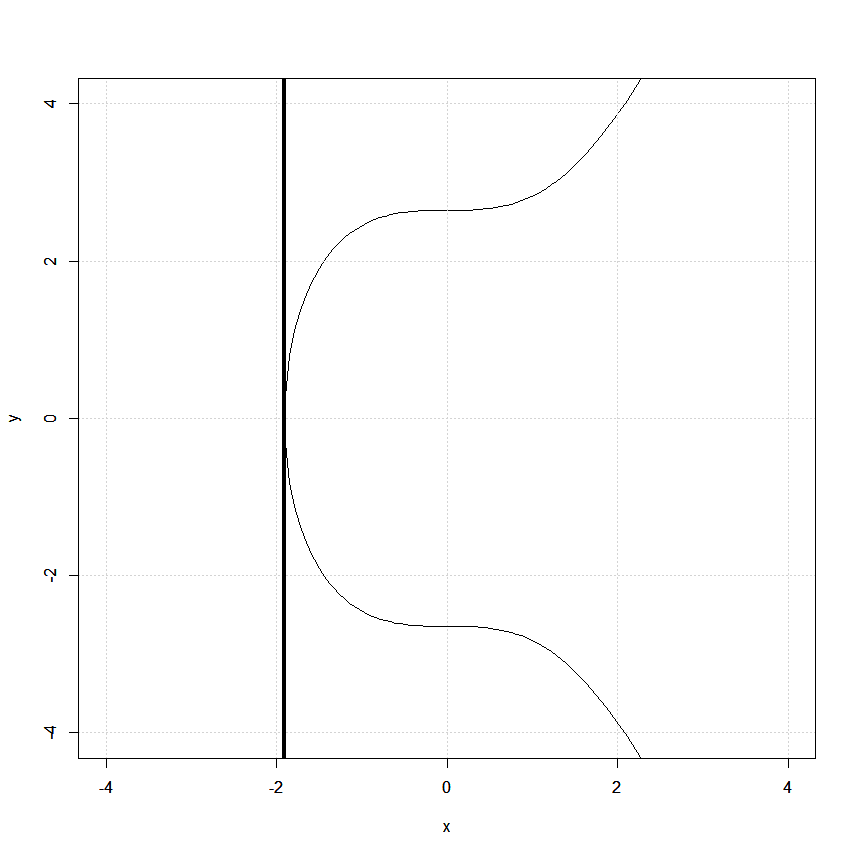
\includegraphics[width=0.9\linewidth]{pictures/elliptic.png}
\caption{Krzywa eliptyczna zastosowana do wyznaczenia wartości G w protokole Bitcoin}
\label{fig:krzywaEliptyczna}
\end{figure}

\section{Podsumowanie} \label{sec:podsumowanieKryptowaluty}
\indent Reasumując za każdą walutą musi stać określony system zabezpieczeń. W przypadku tradycyjnych walut są to centralne instytucje nadzorujące obrót i podaż określonego pieniądza. W przypadku kryptowalut bezpieczeństwo zapewnione jest poprzez zastosowanie prostej w użyciu, aczkolwiek skomplikowanej w budowie kryptografii. Zapewnia to możliwości bardzo szybkiej weryfikacji posiadanych środków, przy bardzo niskim nakładzie pracy. Dodatkowo kryptografia w porównaniu do tradycyjnych metod zabezpieczania pieniądza, nie pozwala na kontrolowanie przez jedną osobę, organizację czy instytucję poprawności danych. To zadanie wykonywane jest przez wszystkich kopaczy w sieci Bitcoin. 


\chapter{Blockchain - rejest transakcji}
\label{blockchain}

\section{Wprowadzenie}
\indent W tym rozdziale przedstawiono oraz wyjaśniono ideę rejestru transakcji, tzw. blockchaina. Opisano strukturę bloku, transakcji oraz wejść i wyjść w transakcji. Rozdział ten opisuje również w jaki sposób tworzone są transakcje, jak są weryfikowane i jakie koszty ponosi się za przekazanie Bitcoinów innemu uczestnikowi sieci. Dodatkowo przedstawiono proces tworzenia oraz dodawania nowego bloku do blockchaina. 

\section{Definicja Blockchain'a}
\label{definicjaBlockchaina}
\indent Łancuch bloków (ang. Blockchain) jest uporządkowaną strukturą zwaną jednokierunkową listą składającą się z bloków transakcji. Listę tę charakteryzuje połączenie wsteczne co oznacza, że blok następny wskazuje na blok poprzedni. Każdy kolejny blok ma przypisaną swoją wysokość w łańcuchu bloków. Wysokość ta ustalana jest na podstawie odległości bloku od pierwszego bloku w łańcuchu. Blok ten, zwany blokiem genezy, stanowi pierwszego \textit{rodzica} oraz wspólnego przodka dla wszystkich bloków w całym łańcuchu\cite{BitcoinAndCryptocurrencyTechnologies}. Idea łańcucha bloków przedstawiona jest na ilustracji \ref{blockchain}.

\indent Pierwszy blok łańcucha bloków w sieci Bitcoin został wygenerowany w 2009 roku i~jako jedyny z bloków zapisany jest w kodzie źródłowym oprogramowania - zapewnienia to zaufanego wspólnego przodka dla wszystkich bloków łańcucha.

\indent Bloki rozpoznaje się na podstawie unikalnego hash'a, który generowany jest przy użyciu algorytmu kryptograficznego SHA256. Wynikowy hash ma 256 bitów i w celu ułatwienia jego odczytu prezentowany jest zazwyczaj w systemie heksadecymalnym. Blok nie zawierają swojego hasha w~nagłówku, co komplikuje szybkie odnajdowanie bloku. Tak by być szybko i łatwo identyfikowalnym, dane o bloku muszą być przetrzymywane w bazie danych zawierającej dodatkowe informacje o łańcuchu bloków. Każdy z węzłów sieci oblicza hash bloku w trakcie jego odbierania. W nagłówku blok zawiera informację tylko o rodzicu, tzn. przechowuje hash rodzica. Poruszając się wstecz przy pomocy tych hash'y powróci się do pierwszego bloku - bloku genezy. 

\indent Hash bloku powstaje na podstawie jego zawartości włączając w to nagłówek bloku, w~którym znajduje się wspomniany hash poprzednika. Powoduje to, iż ingerencja w dane znajdujące się w blokach staje się niemożliwa ze względu na ilość obliczeń jakie należałoby wykonać, aby je zmienić. Jakakolwiek zmiana w bloku rodzica wymusza zmianę w bloku dziecka, dlatego im blok jest starszy tym jest bezpieczniejszy. Taka struktura stanowi podstawę bezpieczeństwa w sieci Bitcoin.

\indent Im blok znajduje się dalej w łańcuchu tym jest stabilniejszy i pewniejszy, natomiast ostatnie bloki, tzn. najświeższe, mogą ulegać zmianom w wyścigu prowadzonym przez kopaczy. W tym samym momencie na ostatni blok może wskazywać wiele nowych bloków wyprodukowanych w trakcie kopania. Taka sytuacja prowadzi do rozgałęzienia się łańcucha bloków. Jest to nieakceptowalne~w opisywanej strukturze, dlatego ostatecznie do łańcucha bloków dołączany zostaje jeden~z wygenerowanych bloków, a reszta bloków zostaje odrzucona. Bardziej szczegółowo problem ten został opisany w podrozdziale \ref{dolaczanieNowegoBloku}.

\begin{figure}[h]
	\begin{center}
  	\begin{tabular}{ | l  c | }
		\hline    
     	Hash bloku & \texttt{000000000000000000a7b47a1e58e456} \\
    			    & \texttt{fd54ae5a30cb92a35ca3e5acee065287} \\ 
    	Wysokość bloku & \texttt{496201} \\ 
    	Rozmiar: & \texttt{1071.607 kB} \\
   	 	Liczba transakcji: & \texttt{2032} \\ \hline
		\textbf{Nagłówek bloku}  &  \\  	 	
   	 	Wersja: & \texttt{0x20000000} \\   	 	
   	 	Hash poprzedniego bloku: &  \texttt{000000000000000000c6dd215947b569} \\
    							 &  \texttt{fa06de2cb856dec643daf5a7e8efc72e} \\ 
		Markle root: 			 & \texttt{b96da6d09865e36e4862b5a612fb1893} \\
								 & \texttt{275d889989feb5a7a217503fd84019e3} \\
   		Czas wykopania: & \texttt{2017-11-26 13:51:02} \\
   		Trudność: & \texttt{1,347,001,430,558.57}\\
   		\hline
   		Transakcje &\\
   		\hline 
 	\end{tabular}
	\end{center}
	
	\begin{center}
	\begin{tabular}{c} 
		\big\Downarrow\
	\end{tabular}
	\end{center}
	
	\begin{center}	
	\begin{tabular}{ | l  c | }
		\hline    
     	Hash bloku & \texttt{000000000000000000c6dd215947b569} \\
    			    & \texttt{fa06de2cb856dec643daf5a7e8efc72e} \\ 
    	Wysokość bloku & \texttt{496200} \\
    	Rozmiar: & \texttt{1062.264 kB} \\
		Liczba transakcji: & \texttt{1036}\\ \hline
		\textbf{Nagłówek bloku} & \\
   	 	Wersja: & \texttt{0x20000000} \\   	 
   	 	Hash poprzedniego bloku: & \texttt{000000000000000000c645c295fbd91d}\\
   	 							 & \texttt{f2f53e0346a4ecf8821abc8cc18fa4b1}\\
		Markle root: 			 & \texttt{c6be2f384d7fa195dfac1ce367ee3a9f}\\
								 & \texttt{9ccfaf9cd337b261be1a0ff0e5d73bc4}\\
   		Czas wykopania: & \texttt{2017-11-26 13:43:52}\\
   		Trudność: & \texttt{1,347,001,430,558.57}\\
   		\hline
   		Transakcje &\\
   		\hline 
 	\end{tabular}
 	\end{center}

	\begin{center}
	\begin{tabular}{c}
		\big\Downarrow
	\end{tabular}
	\end{center} 	

 	\begin{center}
	\begin{tabular}{ | l  c | }
		\hline   
     	Hash bloku &\texttt{000000000000000000c645c295fbd91d} \\
    			    & \texttt{f2f53e0346a4ecf8821abc8cc18fa4b1} \\ 
    	Wysokość bloku & \texttt{496199} \\ 
    	Rozmiar: & \texttt{1059.467 kB} \\
    	Liczba transakcji: & \texttt{1758} \\ \hline
		\textbf{Nagłówek bloku} & \\
		Wersja: & \texttt{0x20000000} \\
   	 	Hash poprzedniego bloku: & \texttt{0000000000000000004f4c7ee2fad2a6}\\
   	 							 & \texttt{51b5bc1e7ce4254fe48490f7a1640dde}\\
		Markle root: 			 & \texttt{20e56ffedbf72d4d729d668037ac1a187} \\
								 & \texttt{0ef937e4ae9491eb7ac7c69f77924407} \\
   		Czas wykopania: & \texttt{2017-11-26 13:43:59} \\
   		Trudność: & \texttt{1,347,001,430,558.57}\\
   		\hline
   		Transakcje &\\
   		\hline 
 	\end{tabular}
 	\end{center}
  	\caption{Przykładowy łańcuch 3 bloków sieci Bitcoin.}
	\label{fig:lancuchBlokow}
\end{figure}	

\section{Struktura i zawartość bloku}
\label{zawartoscBloku}
\indent Każdy blok ma ściśle określoną strukturę, która zawsze jest taka sama i składa się z:
\begin{itemize}
\item[--] rozmiaru bloku,
\item[--] nagłówka bloku,
\item[--] licznika transakcji,
\item[--] transakcji.
\end{itemize}

\indent Pierwsze trzy elementy maja stały lub ograniczony rozmiar. Rozmiar potrzebny na zapis transakcji w bloku zależy od ich ilości i jest zmienny. Poniżej przedstawiono bardziej szczegółowo każdy z elementów bloku. 

\indent Rozmiar bloku zapisany jest jako podstawowa informacja na samym początku bloku. Pozwala to na odczytanie odpowiedniej ilości danych. 

\indent Nagłówek bloku ma zawsze rozmiar 80 bajtów i zawiera informacje dotyczące:
\begin{itemize}
\item[--] wersji protokołu sieci użytej do wygenerowania bloku - 4~bajty;
\item[--] bloku poprzedniego, tzn. jego hash - 32~bajty;
\item[--] podsumowania transakcji reprezentowanej przy pomocy drzewa Merkle - 32~bajty;
\item[--] szacowany czas wykopania bloku - 4 bajty;
\item[--] trudność wykopania bloku przy pomocy określonego algorytmu proof-of-work - 4~bajty;
\item[--] licznik potrzebny dla algorytmu proof-of-work kopania bloku - 4~bajty.
\end{itemize} 

\indent Licznik transakcji wskazuje na ilość transakcji zapisanych w rejestrze bloku i zajmuje od 1 do 9 bajtów.

\indent Ostatnią, ale najważniejszą częścią bloku są transakcje. Zawartość transakcji zostały opisane w osobnym podrozdziale \ref{transakcje}.

\indent Ilustracja \ref{fig:przykladowyBlok} przedstawia rzeczywiste dane jednego z bloków. Dane te zaczerpnięto ze strony blockchain.info pozwalającej na eksplorowanie Bitcoinowego Blockchaina\cite{blockchaininfo}.

\begin{figure}[h]
	\begin{center}	
	\scalebox{1}{
  	\begin{tabular}{ | l  c | }
		\hline    
     	Hash bloku & \texttt{000000000000000000a7b47a1e58e456} \\
    			    & \texttt{fd54ae5a30cb92a35ca3e5acee065287} \\ 
    	Wysokość bloku & \texttt{496201} \\
    	Rozmiar: & \texttt{1071.607 kB} \\
    	Liczba transakcji: & \texttt{2032} \\  \hline
		\textbf{Nagłówek bloku}  &  \\ 
   	 	Wersja: & \texttt{0x20000000} \\
   	 	Hash poprzedniego bloku: & \texttt{000000000000000000c6dd215947b569} \\
    							 & \texttt{fa06de2cb856dec643daf5a7e8efc72e} \\ 
		Markle root: 			 & \texttt{b96da6d09865e36e4862b5a612fb1893} \\
								 & \texttt{275d889989feb5a7a217503fd84019e3} \\
   		Czas wykopania: & \texttt{2017-11-26 13:51:02} \\
   		Trudność: & \texttt{1,347,001,430,558.57}\\
   		\hline
   		Transakcje &\\
   		\hline 
 	\end{tabular}}
	\end{center}
	\caption{Przykładowa rzeczywista zawartość bloku sieci Bitcoin.}
	\label{fig:przykladowyBlok}
\end{figure}
\section{Transakcje i opłaty}
\label{transakcje}

\indent Jednym z najważniejszych elementów w sieci Bitcoin są transakcje, które pozwalają na przekazywanie środków pomiędzy klientami sieci. Jak wspomniano w rozdziale \ref{zawartoscBloku} transakcje są zapisywane w blokach, w łańcuchu bloków. Łańcuch ten jest publicznie dostępny, co implikuje właściwość transakcji jako publicznych. 

\indent Każda nowo powstała transakcja rozgłaszana jest w sieci, gdzie jest weryfikowana przez węzły, a w konsekwencji dodana do nowo tworzonego bloku, który zostaje dołączony do blockchaina. Proces ten jest bardzo pracochłonny i wymaga rozesłania informacji o nowej transakcji w całej sieci. Sieć Bitcoin oparta jest na modelu komunikacji typu P2P (peer-to-peer). Oznacza to, że każdy z węzłów połączony jest z paroma innymi uczestnikami sieci, a z kolei Ci uczestnicy połączeni są z paroma kolejnymi uczestnikami. Powoduje to rozprzestrzenianie się informacji w sieci wykładniczo. Każdy z węzłów sieci po otrzymaniu transakcji weryfikuje ją pod kątem poprawności. W przypadku wykrycia niepoprawnej transakcji jest ona natychmiastowo odrzucana i~przestaje być dalej rozpowszechniana. Komunikacja w sieci Bitcoin jest synchroniczna. Oznacza to, że węzeł, który rozgłosił transakcję dostaje informację zwrotną od węzłów z~nim połączonymi o~poprawności stworzonej transakcji. Kryptografia asymetryczna pozwala na anonimizację węzłów w~sieci. Nie muszą się one znać, ani sobie ufać. Wystarczy, że transakcja jest prawidłowo podpisana, a będzie przekazana dalej. Struktura transakcji oraz proces przekazywania Bitcoinów przy pomocy transakcji są skonstruowane w sposób w pełni zabezpieczający środki. Przekaz nie potrzebuje żadnych dodatkowych zabezpieczeń takich jak, np. szyfrowanie łącza. Może być rozpowszechniany bez jakiegokolwiek szyfrowania, co w porównaniu z~walutami fiducjarnymi jest ogromnym zyskiem\cite{Mastering}.

\indent Struktura transakcji składa się elementów zaprezentowanych w tabeli \ref{tab:strukturaTransakcji}, jednakże najważniejsze z nich to:
\begin{itemize}
\item[--] adresy kluczy publicznych (wejścia do transakcji), reprezentujące źródło środków potrzebnych na pokrycie deklarowanej sumy przekazu;
\item[--] adresy kluczy publicznych (wyjścia z transakcji), reprezentujące cel przekazu.
\end{itemize}
\begin{table}[!h]
\begin{center}
\caption{Struktura transakcji.}
\label{tab:strukturaTransakcji}
\begin{tabular}{{|>{\raggedright\arraybackslash}m{40mm}|m{20mm}|m{80mm}|}}
\hline
	\multicolumn{1}{|>{\centering\arraybackslash}m{40mm}|}{\textbf{Element}} 
    & \multicolumn{1}{>{\centering\arraybackslash}m{20mm}|}{\textbf{Rozmiar (bajty)}} 
    & \multicolumn{1}{>{\centering\arraybackslash}m{80mm}|}{\textbf{Opis}}\\ \hline
	wersja protokołu & \centering{4} & określa użytą wersję prokołu użytą do stworzenia transakcji \\ \hline
	ilość adresów wejściowych & \centering{1-9} & ilość adresów reprezentujących źródło przekazywanych środków \\ \hline
	adresy wejściowe & \centering{zmienna} & adresy reprezentujące źródło przekazywanych środków \\ \hline
	ilość adresów wyjściowych & \centering{1-9} & ilość adresów reprezentujących cel przekazywanych środków \\ \hline
	adresy wyjściowe & \centering{zmienna} & adresy reprezentujące cel przekazywanych środków \\ \hline
	czas blokady & \centering{4} & określa czas, kiedy transakcja może zostać wykonana, zazwyczaj ustawiana na 0 w celu jak najszybszego podpisania\\ 
\hline
\end{tabular}
\end{center}
\end{table}

\indent Przekazywane Bitcoiny nie są fizycznie dostępne na adresach wejściowych, a jedynie są zablokowane kluczem znanym tylko właścicielom tych adresów. Po podpisaniu transakcji środki z adresów wejściowych zostaną zablokowane na rzecz adresów wyjściowych i tylko właściciele tych adresów będą mogli uwierzytelniać kolejne przekazy, używając ich jako adresów wejściowych. 

\indent W celu określenia aktualnie dostępnych środków na adresie wejściowym zliczane są \textit{niewydatkowane bloki wynikowe transakcji} lub \textit{niewydane wyjścia transakcyjne} zwane UTXO (ang. Unspend Transaction Output). UTXO są to niepodzielne oraz jeszcze nie wydane kawałki bitcoinów. Bitcoiny dzielą się na mniejsze kawałki zwane tzw. Satoshi i UTXO mogą składać się z ich wielokrotności. 

\indent W momencie potwierdzania transakcji weryfikowane są wszystkie UTXO przypisane do adresów wejściowych, a następnie po wpisaniu jej do łańcucha bloków rejestrowany jest nowy zablokowany UTXO przypisany do adresu wyjściowego. Jak pisano wcześniej UTXO może zostać odblokowany jedynie przez jego właściciela. W sieci Bitcoin nie istnieje jeden główny bilans wszystkich adresów. Podczas realizacji każdej z transakcji sprawdzany jest cały łańcuch bloków i~sumowane są wszystkie UTXO należące do określonego klucza publicznego. Właściciel UTXO podczas jego użycia musi wydać całą zablokowaną sumę Satoshi, dlatego też chęć przelania tylko części środków na UTXO powoduje stworzenie wielu nowych UTXO. Część z nich wskazywać będzie na adresy wyjściowe, a część jako reszta z UTXO będzie wskazywać na adres nadawcy transakcji. Bardzo często zdarza się sytuacja, w której to właściciel wielu UTXO chce przelać środki na jeden adres. W takim przypadku dozwolone jest połączenie tych jednostek w celu osiągnięcia oczekiwanej sumy bitcoinów i przekazania jej na adres odbiorcy. 

\indent Każdy z bloków zawiera jedną transakcję stworzoną przez jednego uczestnika sieci - zwycięskiego kopacza, który otrzymuje profity z tytułu podpisania bloku. Jest to zawsze pierwsza transakcja tzw. \textit{coinbase}. Proces ten został krótko opisany w podrozdziale \ref{dolaczanieNowegoBloku}.

\indent Wszystkie adresy wejściowe można traktować jako punktory do transakcji wyjściowych, zrealizowanych oraz niezrealizowanych (z nich powstają UTXO). Zrealizowane transakcje zawierają również odblokowane skrypty, co pozwala na przekazanie ich dalej. Należy podkreślić, że adresy wejściowe nie niosą informacji o ilości posiadanych środków, a jedynie informację o miejscu, w którym można się o tym dowiedzieć. Poniżej, w tabeli \ref{tab:strukturaWyjscia}, przedstawiono strukturę wyjścia transakcji.
\begin{table}[!h]
\begin{center}
\caption{Struktura wyjścia transakcji.}
\label{tab:strukturaWyjscia}
\begin{tabular}{{|>{\raggedright\arraybackslash}m{40mm}|m{20mm}|m{80mm}|}}
\hline
	\multicolumn{1}{|>{\centering\arraybackslash}m{40mm}|}{\textbf{Element}} 
    & \multicolumn{1}{>{\centering\arraybackslash}m{20mm}|}{\textbf{Rozmiar (bajty)}} 
    & \multicolumn{1}{>{\centering\arraybackslash}m{80mm}|}{\textbf{Opis}}\\ \hline
	kwota & \centering{8} & ilość Bitcoinów przedstawionych w Satoshi \\ \hline
	rozmiar skryptu blokującego & \centering{1-9} & długość skryptu blokującego przedstawiona w bajtach \\ \hline
	skrypt blokujący & \centering{zmienna} & skrypt określający warunki do spełnienia w celu odblokowania wyjścia \\ \hline
\end{tabular}
\end{center}
\end{table}

\indent Transakcje zazwyczaj tworzone za pomocą klienta Bitcoin, co jest wygodnym i bezpiecznym sposobem przekazywania środków. Podczas tworzenia transakcji aplikacja ta dba, aby w transakcji znalazły się wszystkie wymagane informacje. W tabeli \ref{tab:strukturaTworzeniaTransakcji} przedstawiono strukturę tworzenia transakcji.
Pozwala ona spełnić wszystkie warunki określone w tabeli \ref{tab:strukturaWyjscia} przez wyjście transakcji.

\begin{table}[!h]
\begin{center}
\caption{Struktura wyjścia transakcji.}
\label{tab:strukturaTworzeniaTransakcji}
\begin{tabular}{{|>{\raggedright\arraybackslash}m{40mm}|m{20mm}|m{80mm}|}}
\hline
	\multicolumn{1}{|>{\centering\arraybackslash}m{40mm}|}{\textbf{Element}} 
    & \multicolumn{1}{>{\centering\arraybackslash}m{20mm}|}{\textbf{Rozmiar (bajty)}} 
    & \multicolumn{1}{>{\centering\arraybackslash}m{80mm}|}{\textbf{Opis}}\\ \hline
	hash transakcji & \centering{32} & punktor do transakcji zawierającej UTXO do wydania \\ \hline
	indeks wyjścia & \centering{4} & numer indeksu UTXO do wydania \\ \hline
	rozmiar skryptu odblokowującego & \centering{1-9} & długość skryptu odblokowującego wyrażona w bajtach \\ \hline
	skrypt odblokowujący & \centering{zmienna} & skrypt spełniający wszystkie wymagane warunki skryptu blokującego UTXO \\ \hline
	numer sekwencji & \centering{4} & aktualnie nieużywana funkcjonalność wymiany Tx \\ \hline
\end{tabular}
\end{center}
\end{table}

\indent Za każdą przeprowadzaną transakcję trzeba ponieść koszty operacyjne. W przypadku Bitcoina jest to opłata dla górników mająca zachęcać do kopania. Wielkość opłaty nie zależy od ilość przekazywanych Bitcoinów, a od wielkości stworzonej transakcji. Oznacza to, że osoba, która posiada wiele UTXO i chce je skonsumować w jednej transakcji musi zapłacić wyższą opłatę. Wynika to z faktu, że górnik w celu weryfikacji posiadanych UTXO musi wykonać dużo więcej pracy, niż gdyby transfer odbywał się z jednego UTXO. Górnicy bardzo często ustalają kryteria i tworzą priorytety transakcji, które chcą przetwarzać. W~niektórych przypadkach może się okazać, że przez zbyt niską opłatę żaden z~górników nie będzie podejmował się wyzwania sprawdzenia i~podpisania konkretnej transakcji. Jeżeli transakcja nie zostanie podpisana przez górnika nie znajdzie się w~wytwarzanym bloku. Transakcja ta \textit{wisieć} będzie w sieci do czasu przetworzenia przez któregoś z kopaczy.

\section{Dołączania kolejnego bloku z transakcjami}
\label{dolaczanieNowegoBloku}

\indent Wszystkie transakcje rozsyłane po sieci trafiają do górników, którzy gromadzą je w~celu zbudowania nowego bloku. Transakcje te są jedynie kandydatami do znalezienia się w~bloku, a które z nich znajdą się w zbudowanym bloku zależy od priorytetów górnika. 

\indent Przypuszczając sytuację, w której górnik otrzymuje wiadomość o powstaniu nowego bloku $X$, nad który też pracował, akceptuje otrzymane rozwiązanie i podejmuje się wyzwania skonstruowania bloku $X+1$. Porównuje transakcje z bloku $X$ z otrzymanymi transakcjami. Redukuje ich ilość, tak by nie próbować umieszczać tych samych transakcji w kolejnym bloku i próbuje wytworzyć kolejny blok. Sprawdza wszystkie transakcje przeznaczone do umieszczenia w bloku pod względem poprawności, a następnie generuje transakcję zwaną \textit{coinbase}. 

\indent Transakcja \textit{coinbase} zawiera w wejściu do transakcji nowe bitcoiny, które są nagrodą za wygenerowany blok oraz opłaty wniesione przez zleceniodawców transakcji. Ilość nowych bitcoinów zależy ilości istniejących bloków w sieci. Nagroda ta zmniejsza się wraz z~ich ilością. Na początku istnienia sieci wynosiła ona 50 BTC i zmniejsza się o połowę co 210 tys. bloków. Aktualnie wynosi 12.5 BTC. Każdy górnik po otrzymaniu bloku sprawdza, czy górnik, który wytworzył blok nie oszukał generując transkację \textit{coinbase}. W przypadku oszustwa taki blok zostaje odrzucony, a praca i koszty poniesione przez górnika zostają niepokryte. W przeciwnej sytuacji, kiedy to górnik poprawnie wykonał swoją pracę, bitcoiny zwarte w tej transakcji trafiają na adres w niej określony. Zazwyczaj tym adresem jest adres górnika.

\indent Po dodaniu transakcji \textit{coinbase} tworzony jest nagłówek bloku, który zawiera wszystkie dane informacje opisane w rozdziale \ref{zawartoscBloku}. W nagłówku dostępny jest hash bloku poprzedniego oraz hash drzewa Merkle, który pozwala na szybką weryfikację \textit{zaksięgowania} transakcji w bloku. Algorytm tworzenia drzewa Merkle wymaga istnienia parzystej liczby transakcji w bloku. W przypadku zawarcia nieparzystej ilości transakcji w bloku, ostatnia z nich jest duplikowana na potrzeby stworzenia drzewa.

\indent Kolejnym krokiem tworzenia bloku jest podpisanie go poprzez znalezienie rozwiązania określonego algorytmu \textit{proof-of-work}. Algorytm ten polega na wielokrotnym mieszaniu nagłówków bloków oraz jednej zmiennej do momentu uzyskania hash'a o określonych właściwościach. Hash'e generowane są przy pomocy algorytmu kryptograficznego wspomnianego w rozdziale \ref{definicjaBlockchaina} zwanego funkcją skrótu SHA256. Warunki do spełnienia mogą się zmieniać wraz ze zmianami w sieci. Przykładową własnością docelową poszukiwanego hasha może być, aby hash ten był mniejszy niż ustalony próg celu, tzn. musi być mniejszy niż określony hash.

\indent Po odnalezieniu hash'a bloku $X+1$, zostaje on rozsyłany po sieci w celu ogłoszenia jego wygenerowania. Klienci sieci otrzymują tę informację i weryfikują poprawność nowego bloku. Oznacza to, że każdy węzeł sieci musi przeprowadzić wiele testów weryfikacyjnych zanim wyśle blok do połączonych węzłów. Po zaakceptowaniu bloku przez węzeł, zostaje on dodany do lokalnego łańcucha i wysłany dalej. W przypadku kiedy węzeł otrzyma blok $Y$ od innego węzła wskazujący na ten sam poprzedni blok($X$), co blok $X+1$, blok $Y$ zostaje odrzucony.

\indent W tak skonstruowanym systemie może się wydarzyć sytuacja, w której dwóch górników jednocześnie zacznie rozsyłać poprawny blok po sieci. Oznaczać to będzie, że węzły zatwierdzą blok \textit{górnika 1} oraz blok \textit{górnika 2} i powstanie rozwidlenie sieci. W takich sytuacjach sieć oczekuje na wyprodukowanie kolejnego bloku, który użyje jednego z bloków wyprodukowanych przez \textit{górnika 1} lub \textit{górnika 2} w celu odnalezienia globalnego consensus. Zachowanie sieci w tym przypadku zależy od wskazania w tym generowanym bloku hasha bloku poprzedniego. Dłuższy łańcuch bloków jest przez sieć traktowany jako ważniejszy i nieużyty blok w tym łańcuchu zostaje przegłosowany, a konsekwencji staje się blokiem sierocym. Łańcuchy bloków stworzone przez węzły na podstawie przegłosowanego bloku zostają skorygowane i zastosowany zostaje dłuższy łańcuch bloków.

\section{Podsumowanie}

\indent Konkludując Blockchain jest strukturą zbudowaną z bloków wstecznie połączonych. Każdy blok z łańcucha zawiera informacje o zrealizowanych transakcjach oraz o hashu bloku poprzedniego. Transakcje składają się z wejść do transakcji oraz wyjść z transakcji. Wejścia są punktorami do niewydanych wyjść transakcji z poprzednich bloków, a wyjścia transakcji wskazują na adresy uczestników sieci, do których mają trafić bitcoiny. Bloki generowane są z transakcji przez górników, którzy walczą w wyścigu o nagrodę w postaci nowych bitcoinów oraz opłat transakcyjnych. Nowo wygenerowane bloki dołączane są do łańcucha bloków w procesie znajdowania globalnego consensusu w sieci.

\chapter{Przegląd metod analiz sieci złożonych (też temporalnych) oraz analiz blockchaina}
Czym jest analiza sieci, jakie były analizy, metody analiz grafów.
Nie tylko analizuje się sieci statyczne, ale temporalne i wielowarstwowe.
Jak analizować blockchain, co zostało zrobione w kontekście jego analizy?


\chapter{Analiza blockchaina Bitcoin}

\section{Wprowadzenie}

\indent W niniejszym rozdziale przedstawiono część eksperymentalną pracy. Sformułowano cel badawczy oraz określono zakres przeprowadzanych analiz. Przybliżono również sposób tworzenia sieci oraz określono związek pomiędzy węzłami sieci. Następie opisano przeprowadzone analizy wraz z wnioskami.

\section{Plan badań}

\indent Celem przeprowadzanego eksperymentu jest analiza rejestru transakcji w~sieci Bitcoin. Podjęto próbę określania cech sieci, które pozwalają na stworzenie charakterystyki jej rozwoju. Przy pomocy metod analizy sieci złożonych zbadano trendy zmian zachodzących w sieci oraz zaobserwowano zdarzenia nietypowe, odbiegające od wyznaczonego trendu. 

\indent Na potrzeby realizacji eksperymentu wyznaczono po dziesięć węzłów startowych w~sieci w dziesięciu okresach. Wybrano bloki z~łańcucha bloków dołączone jako ostatnie w dziesięciu kwartałach w~okresie od \textit{2015-03-31} do \textit{2017-06-30}. Następnie z~każdego z~bloków dla każdego okresu wybrano po dziesięć transakcji, które stały się węzłami startowymi dla badanej sieci. Oznacza to, że analizę przeprowadzono na stu próbach po sto tysięcy węzłów każda. Ilość oraz wielkość prób zmniejsza ryzyko natrafienia na próbę  niereprezentacyjną.

\indent Każdą sieć, która stanowi próbę do badań, stworzono zaczynając od węzła startowego wstecz. Każdy węzeł reprezentuje transakcję wskazując na jej adres. Jak opisano w~podrozdziale \ref{transakcje} transakcje zawierają adresy wejściowe oraz adresy wyjściowe. W~podrozdziale \ref{transakcje} podkreślono również fakt, że adresy wejściowe są jedynie referencjami na adresy wyjściowe, co implikuje właściwość związków pomiędzy transakcjami. W celu łatwiejszego zrozumienia sposobu budowania sieci w tabeli \ref{tab:zwiazekTransakcji} przedstawiono dwie połączone transakcje, na przykładzie których zauważyć można, że transakcja $N-1$ zawiera adres wyjściowy identyczny jak jeden z adresów wejściowych transakcji $N$. Oznacz to, że transakcje te są połączone i stanowią dwa węzły sieci połączone krawędzią. Wykorzystując tę zależność każdą próbkę stworzono poprzez znalezienie sto tysięcy połączeń pomiędzy transakcjami na podstawie adresów wejściowych i adresów wyjściowych zaczynając od początkowego adresu transakcji. Na ilustracji \ref{fig:siec} przedstawiono przykładowy generyczny wycinek każdej z stworzonych sieci zaczynając od węzła $N$, natomiast na ilustracji \ref{fig:graf} przedstawiono rzeczywisty graf jednej z próbek.

\begin{table}[H]
\begin{center}
\caption{Związek pomiędzy transakcjami.}
\label{tab:zwiazekTransakcji}
\begin{tabular}{|l|l|l|l|}
\hline
	\multicolumn{2}{|c|}{Transakcja N-1} 
   &\multicolumn{2}{|c|}{Transakcja N}  \\
\hline
Adresy wejściowe & Adresy wyjściowe &Adresy wejściowe & Adresy wyjściowe\\
\hline
W4 & W2 & W2 & W1 \\
&& W3 & \\
\hline 
\end{tabular}
\end{center}
\end{table}

\begin{figure}[H]
\begin{center}
\centering
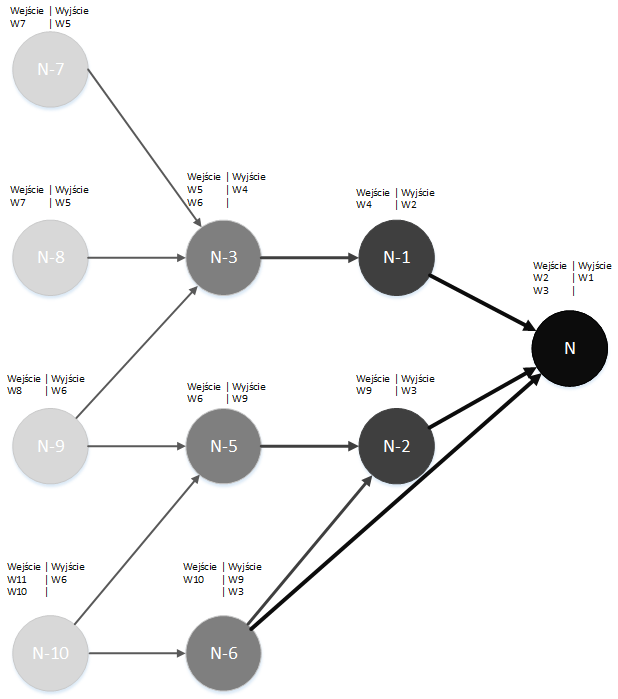
\includegraphics[width=1\linewidth]{pictures/visio/siec.png}
\caption{Przykładowy wycinek próbki sieci.}
\label{fig:siec}
\end{center}
\end{figure}

\begin{figure}[H]
\begin{center}
\centering
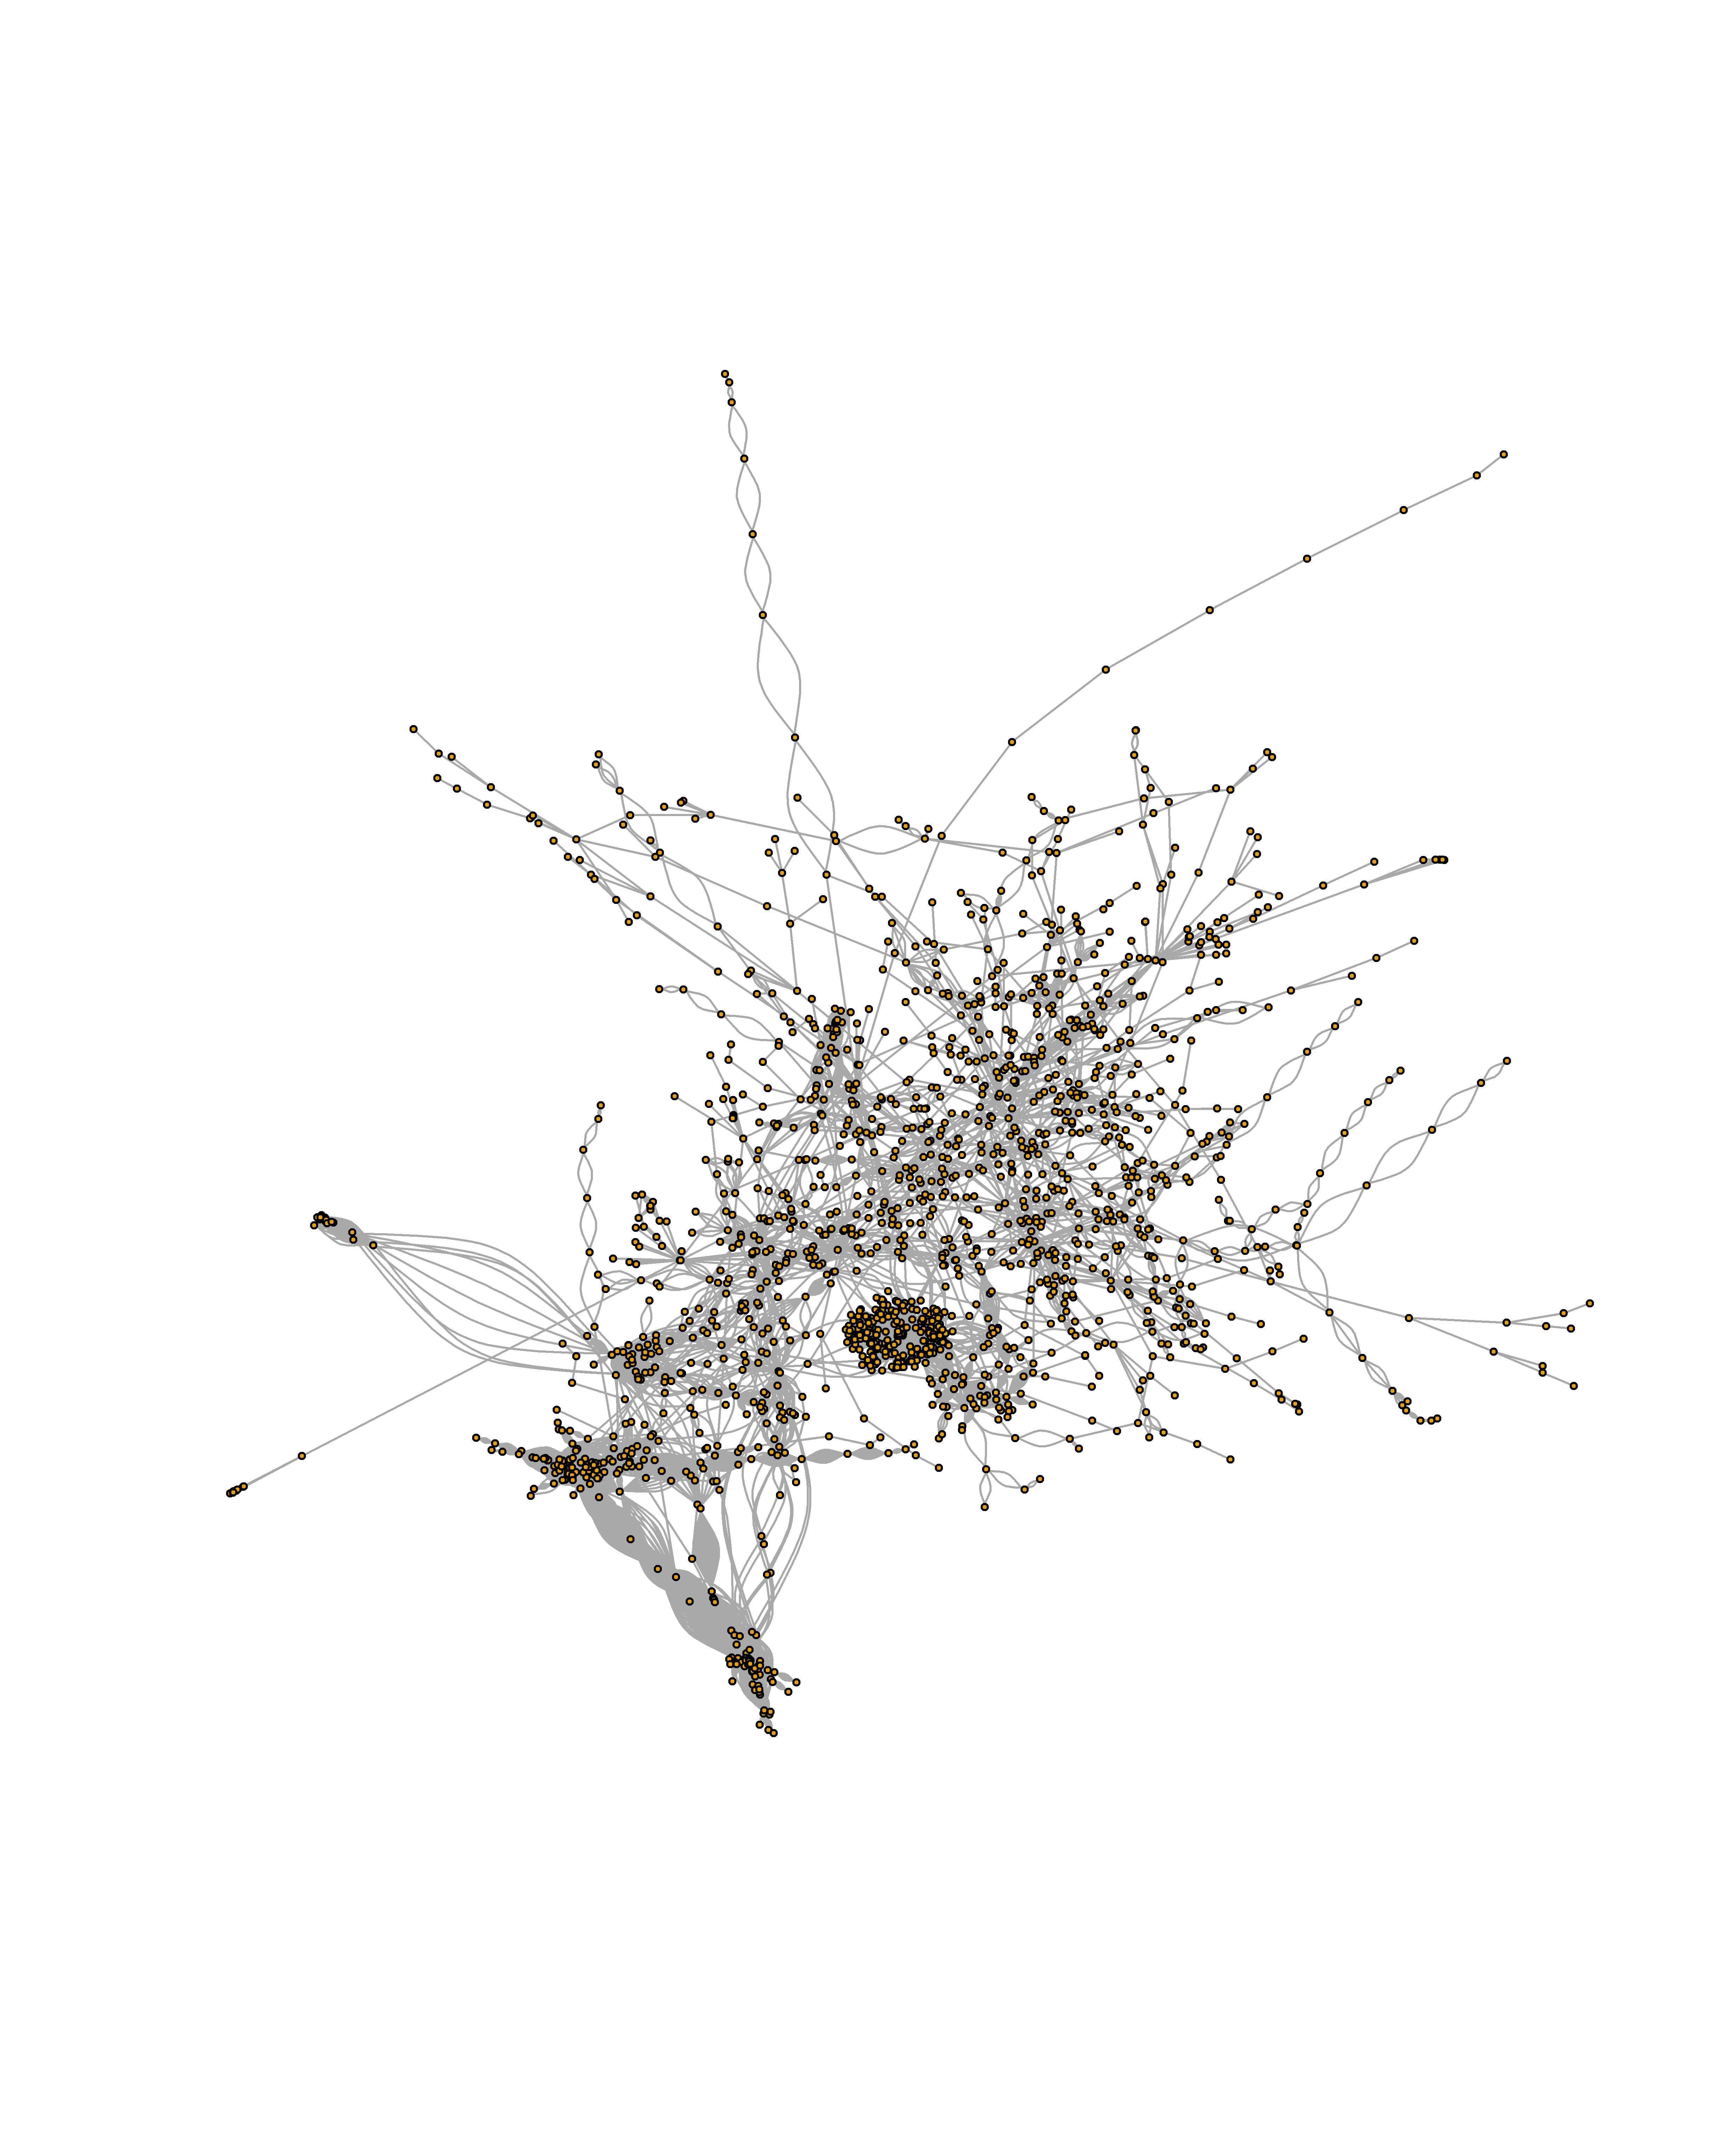
\includegraphics[width=1\linewidth]{pictures/graph/graph.png}
\caption{Wizualizacja grafu składającego się ze stu tysięcy połączeń.}
\label{fig:graf}
\end{center}
\end{figure}

\newpage
\indent Przeprowadzone badania podzielono na dwie grupy pod względem reprezentowanych cech sieci. Pierwsza grupa reprezentuje analizę sieci przy pomocy algorytmów generycznych dla sieci złożonych. Algorytmy te nie silnie związane z problematyką fachową sieci, jednakże pozwalają na zbadanie podstawowych własności każdej z sieci. W~ramach analizy dla każdej próbki zbadano:
\begin{itemize}
\item[--] średnicę sieci,
\item[--] średnią długość ścieżek,
\item[--] średni stopień węzłów,
\item[--] średnią centralność węzłów.
\end{itemize}
Druga grupa przeprowadzonych badań pozwoliła na analizę sieci pod kątem jej specyficznych własności, które są bardzo mocno związane z jej problematyką. W ramach analizy dla każdej próbki zbadano:
\begin{itemize}
\item[--] średnią wartość transakcji,
\item[--] liczbę bloków potrzebnych do stworzenia próbki,
\item[--] średnią różnicę czasów kolejnych transakcji,
\item[--] różnice czasu granicznych transakcji.
\end{itemize}

\indent Badania z grupy pierwszej przeprowadzono przy pomocy biblioteki \textit{Igraph}, natomiast algorytmy potrzebne do przeprowadzenia badań z grupy drugiej zostały przygotowane samodzielnie.

\section{Eksperyment}
W ramach przeprowadzonych badań dla każdej z metryk stworzono mapę cieplną przedstawiającą wartości poszczególnych właściwości sieci. Na wykresie zaprezentowano również średnią wartość dla każdego z okresu wraz z odchyleniem standardowym, z którego stworzono regresję liniową. Na podstawie tych danych przeprowadzono analizę oraz określono trend zmian w sieci.  

\subsection{Badanie średnicy sieci}
\label{srednica_sieci}
\indent Średnica sieci jest długością $max_{u,v}d(u,v)$ najdłuższej ścieżki znalezionej wśród najkrótszych ścieżek pomiędzy którymikolwiek dwoma węzłami sieci $(u,v)$, gdzie $d(u,v)$ jest długością grafu. Długość grafu jest minimalną długością ścieżki (stworzonej z węzłów) potrzebnej do połączenia dwóch określonych węzłów. Inaczej mówiąc średnica grafu jest maksymalną ilością węzłów jakie trzeba pokonać by przejść z jednego węzła do drugiego.

\indent Dla badanej sieci oznacza to maksymalną ścieżkę połączonych transakcji, a co za tym idzie, maksymalną krotność przekazywania pomiędzy adresami publicznymi Bitcoinów. Na podstawie wartość długość ścieżki można wnioskować o własnościach sieci, takich jak na przykład jej gęstości.

\indent Na rysunku \ref{fig:s1} przedstawiono mapę ciepła średnicy sieci dla każdej z próbek. Na jej podstawie można wnioskować, że dla większości przypadków próbki w poszczególnych okresach są zbliżone. Zaobserwować można również, że w każdym z okresów istnieją pojedyncze sieci mocno odbiegające od reszty. Jedyną z tych anomalii jest średnica sieci dla próbki zaczynającej się od transakcji szóstej, która została zrealizowana \textit{2017-03-31}. Istnieje prawdopodobieństwo, że jest to transakcja realizowana w ramach wielokrotnego przesyłania Bitcoinów przez jednego właściciela pomiędzy własnymi adresami w celu próby ukrycia ich źródła.

\indent Na wykresie \ref{fig:s2} przedstawiono regresję liniową na podstawie średniej średnicy dla okresu z odchyleniem standardowym. Z~wykresu wynika, że gęstość sieci rośnie w czasie, o czy świadczy trend spadkowy średnicy sieci. Wzrost gęstości oznacza, że w sieci występuje coraz więcej krawędzi w stosunku do ilości węzłów. Dla sieci Bitcoin wzrost gęstości sieci oznacza wzrost ilość transakcji realizowanych na pojedyncze adresy publiczne, w krótszym czasie. Można zatem wnioskować, że w czasie Bitcoiny coraz częściej gromadzone są na pojedynczych adresach. Odchylenia standardowe widoczne na \ref{fig:s2} wynikają z pojedynczych próbek mocno odbiegających od średniej. Odrzucenie po dwie z próbek (najwyżej oraz najniżej wartościowanych) z każdego okresu zniwelowałoby znacząco rozpiętość odcyhlenia standardowego. Przykładem może być wcześniej omawiana próbka zaczynająca się od transakcji $T6$ z okresu \textit{2017-03-31}. 

\begin{figure}[H]
\centering
  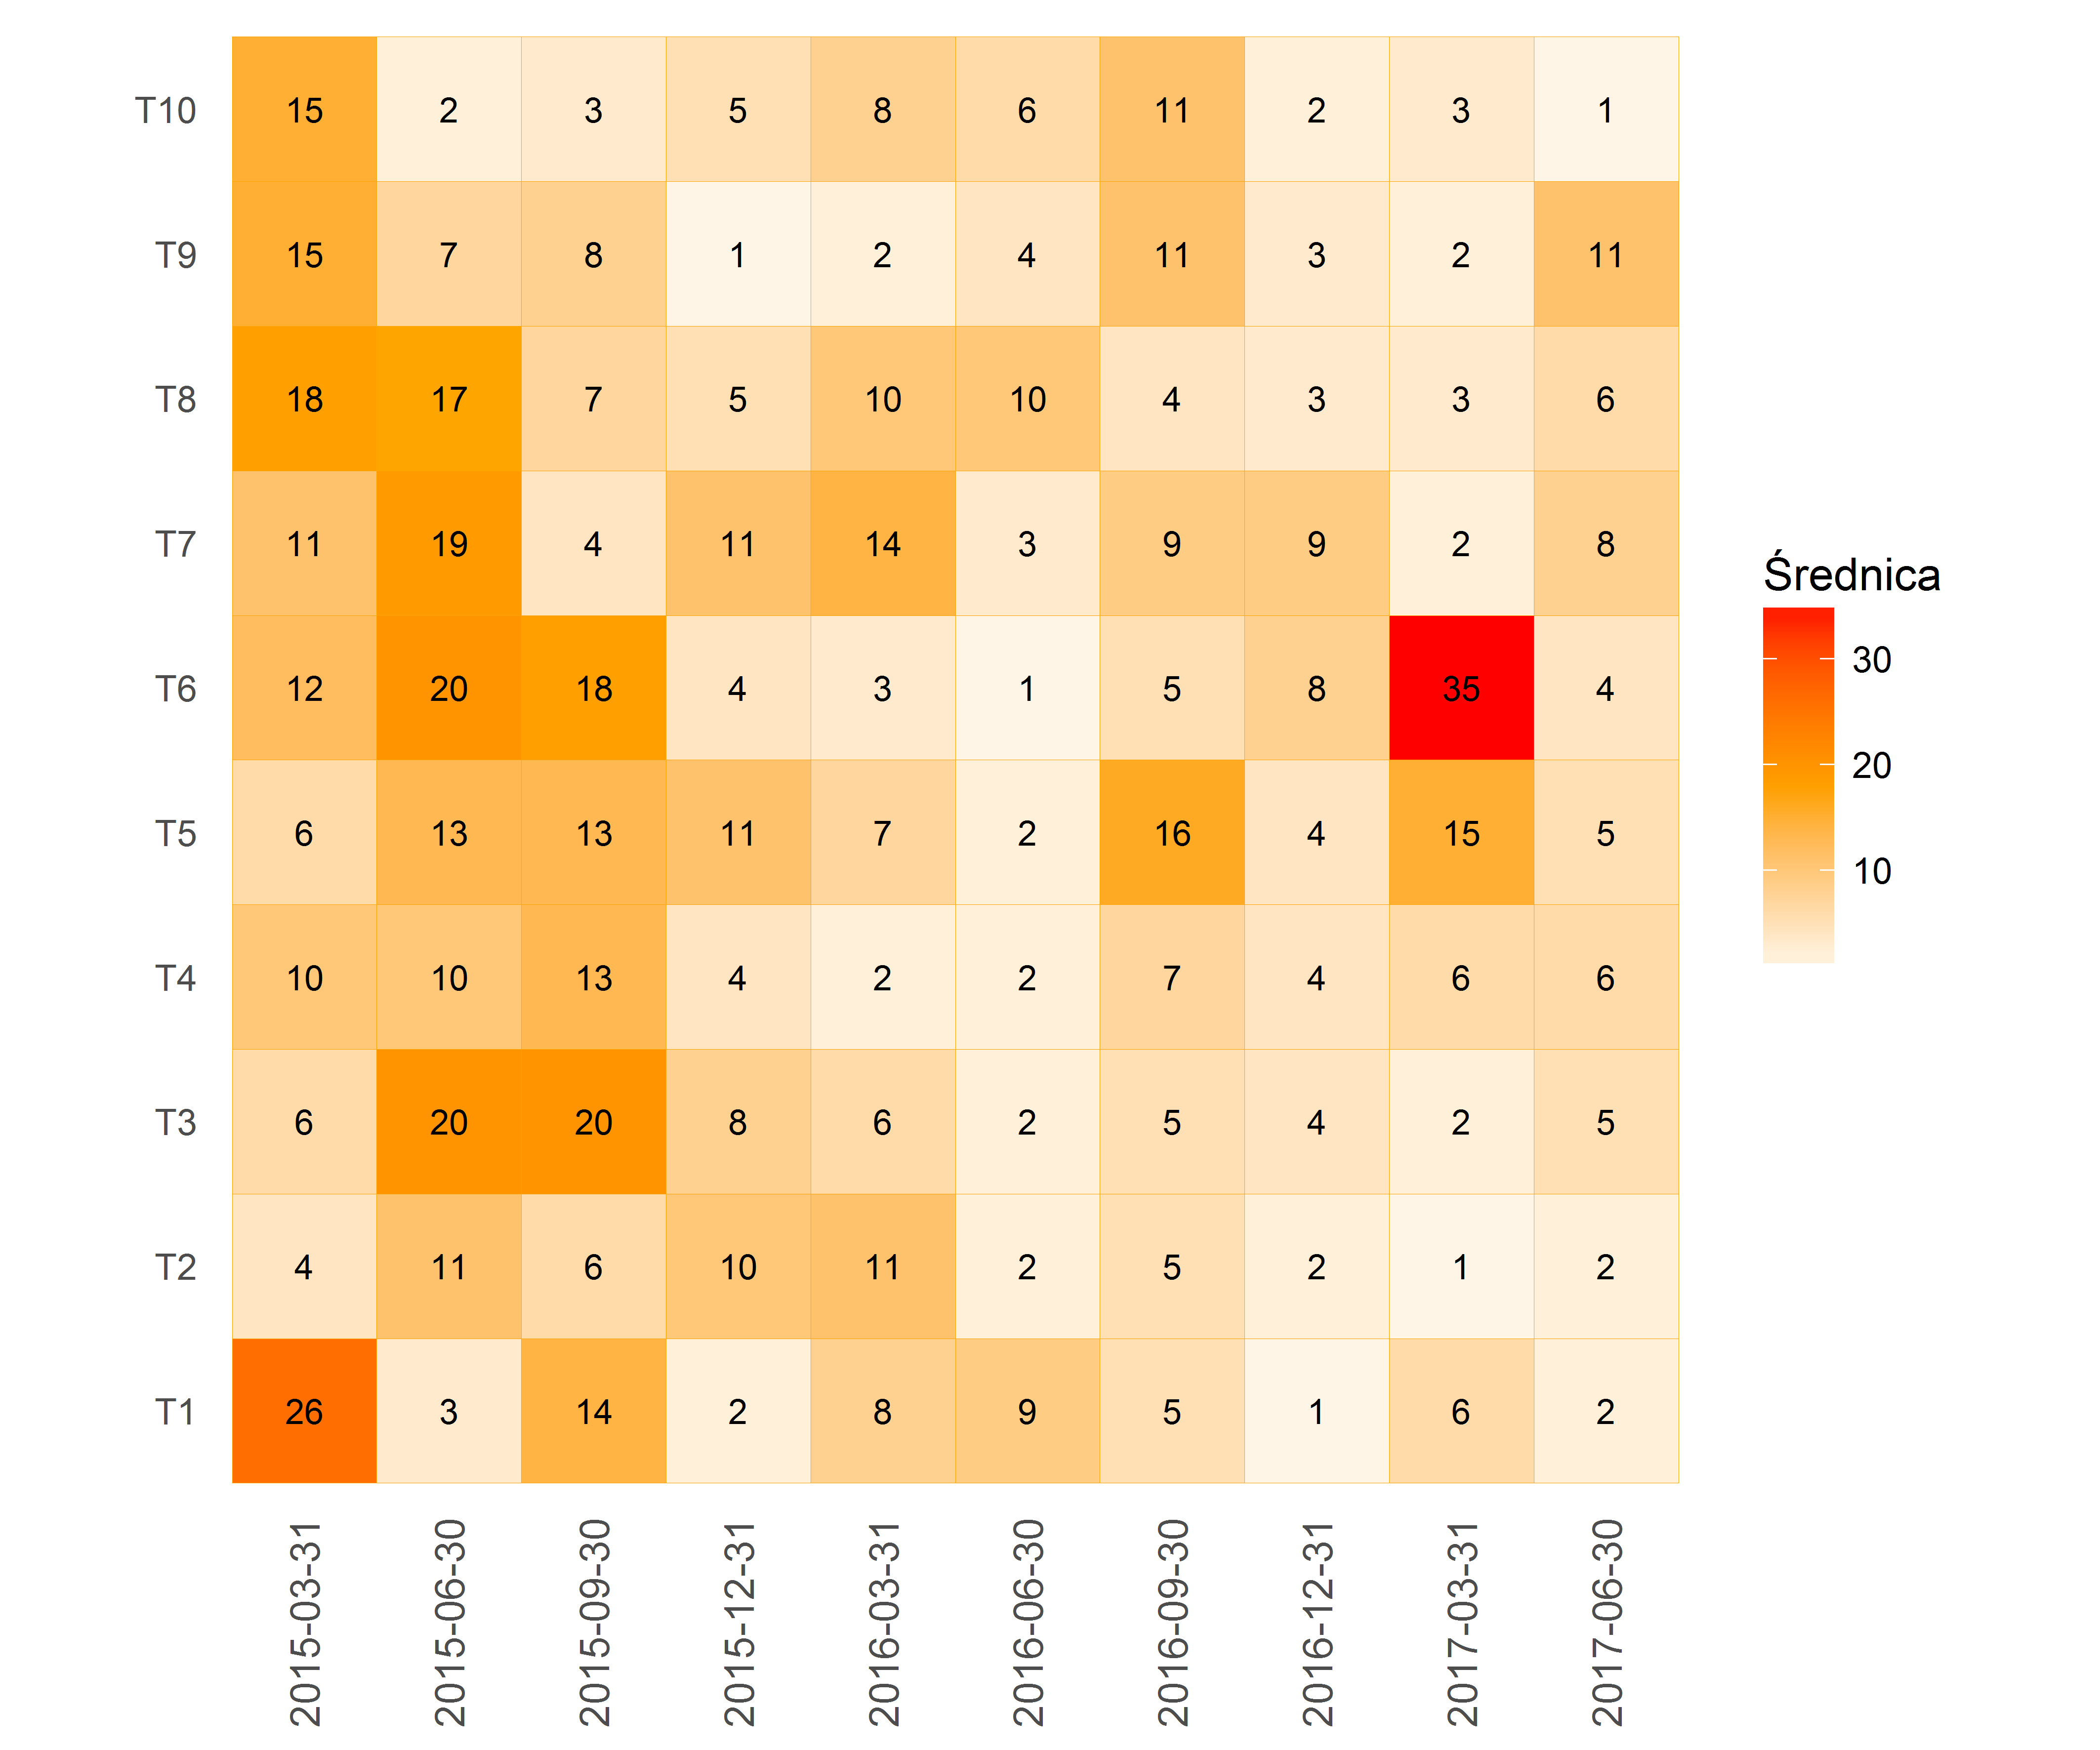
\includegraphics[width=0.9\linewidth]{pictures/srednica/srednica_hm.png}
  \caption{Mapa cieplna średnicy sieci dla 10 transakcji w 10 okresach.}
  \label{fig:s1} 
\end{figure}

\begin{figure}[H]
\centering
  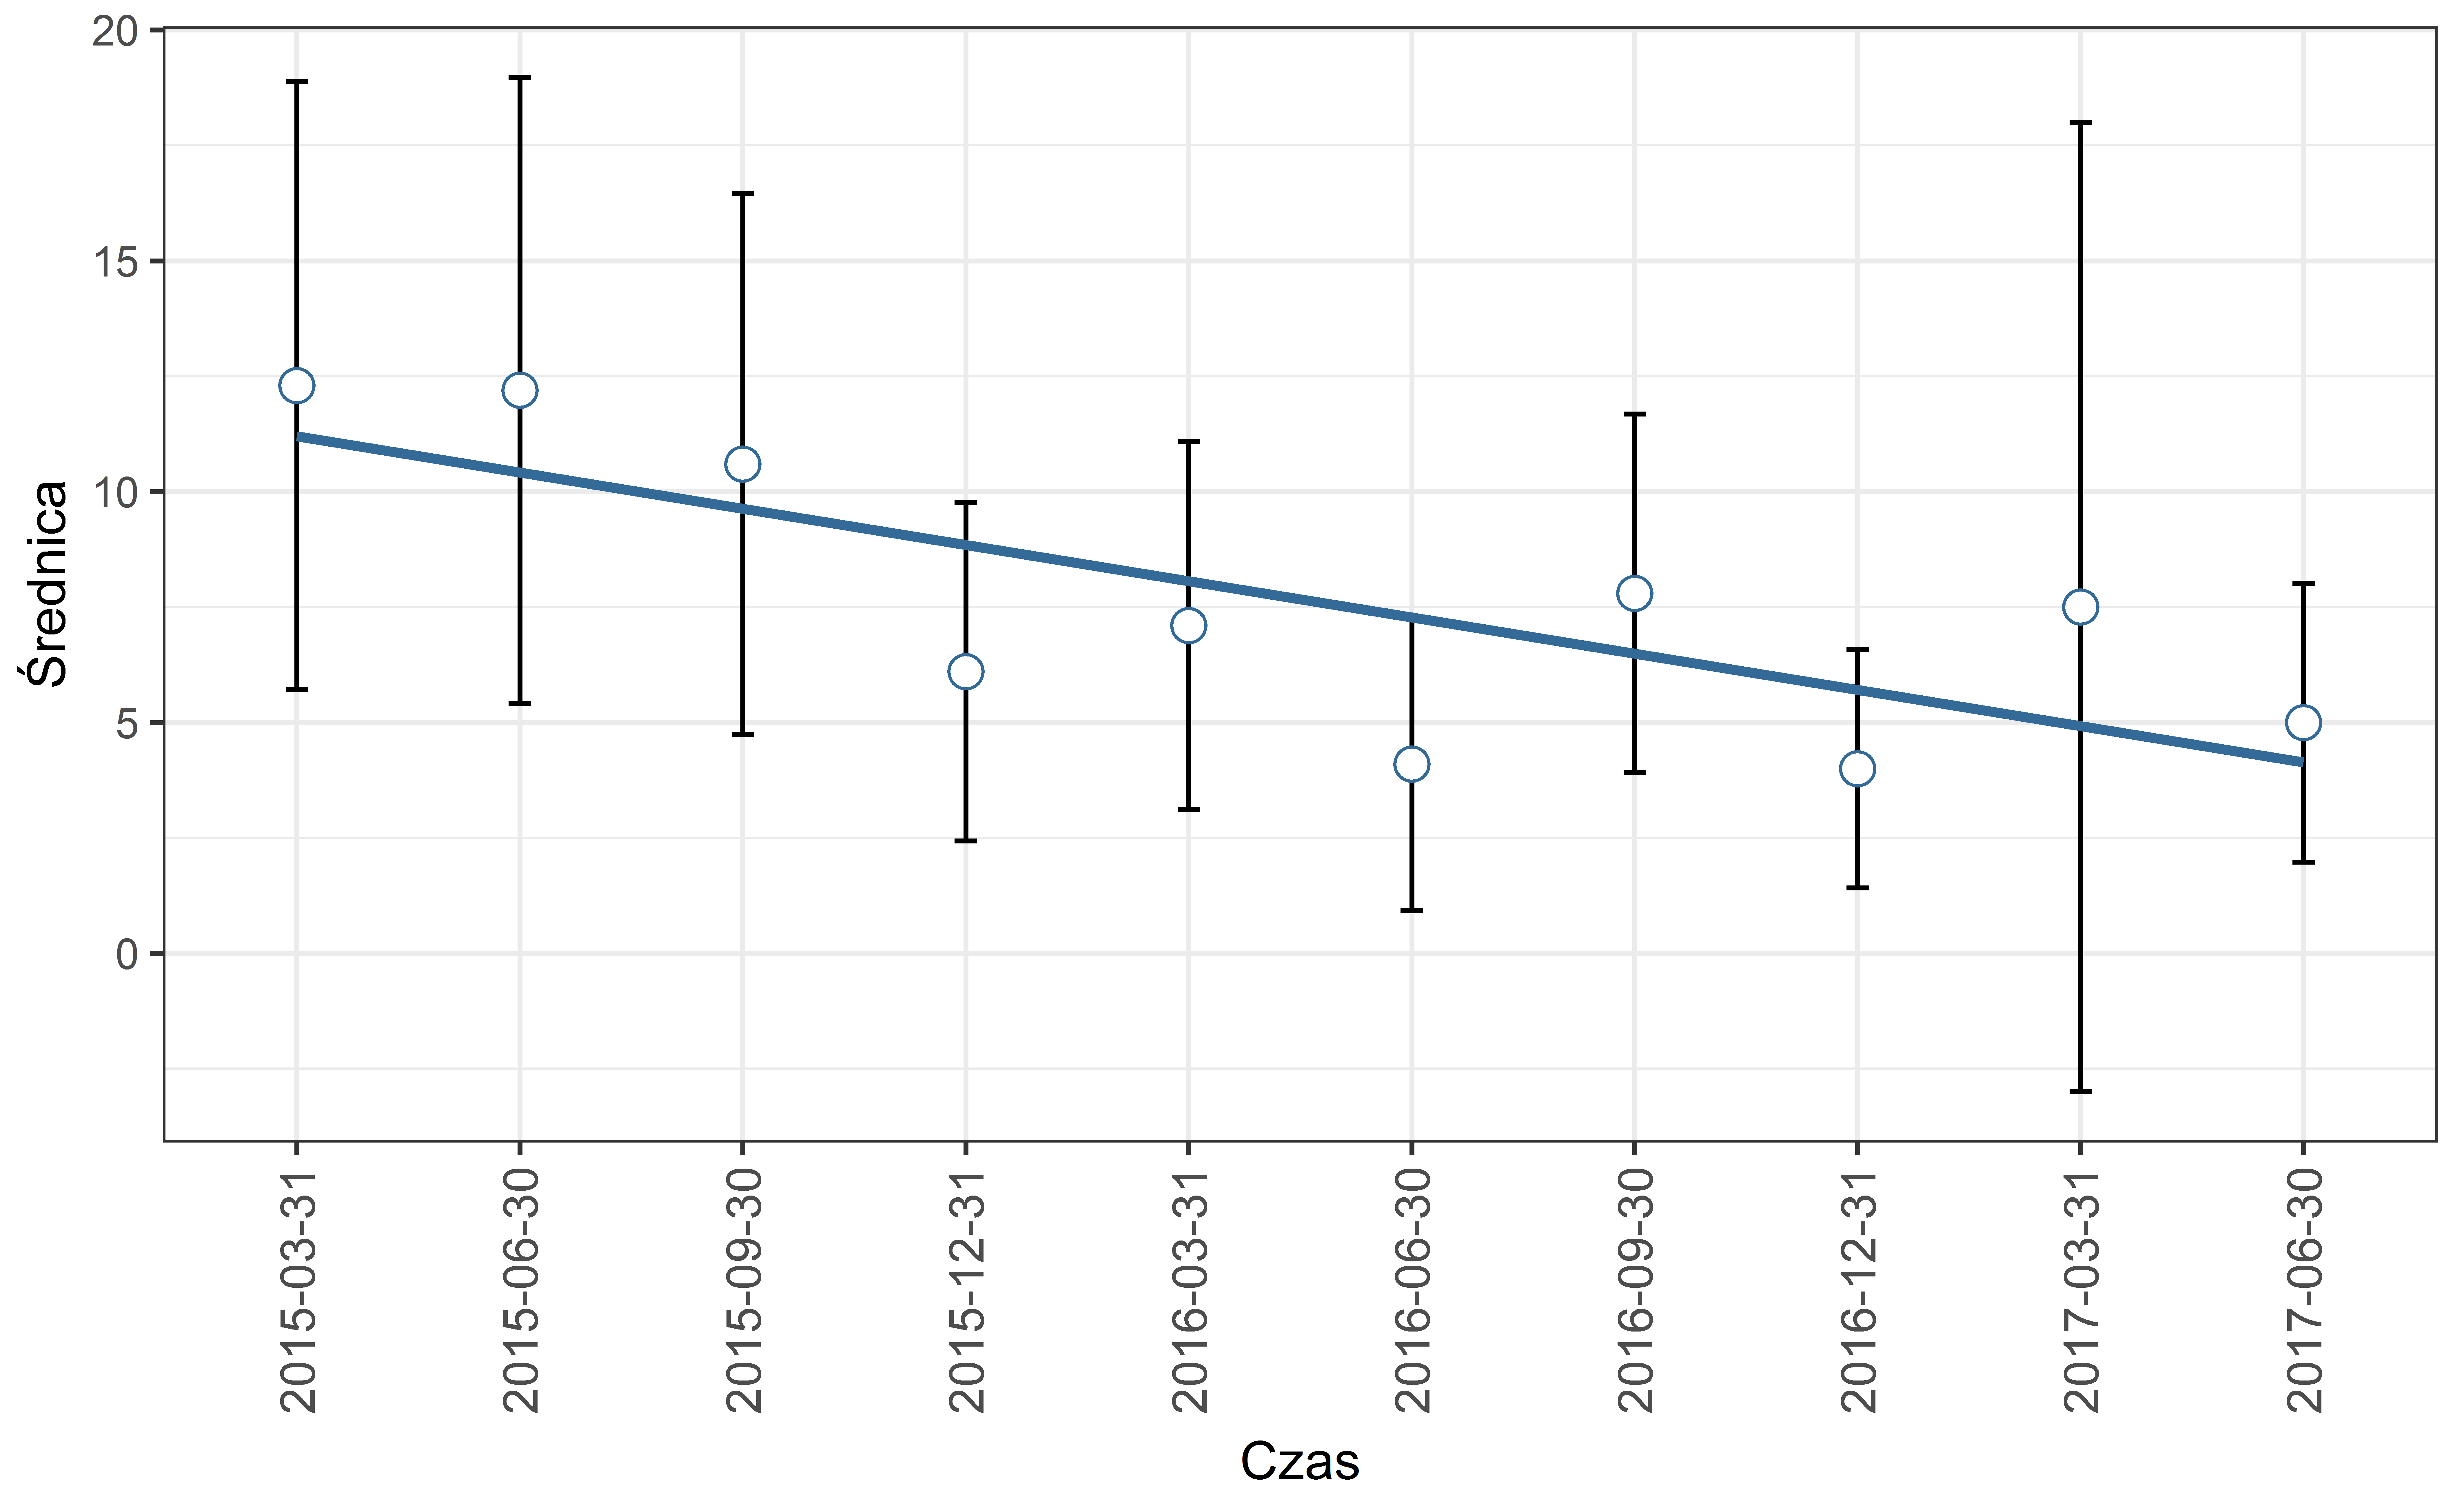
\includegraphics[width=0.9\linewidth]{pictures/srednica/srednica_sda.png}
  \caption{Regresja liniowa średniej średnicy sieci dla 10 okresów z odchyleniem standardowym.}
  \label{fig:s2}
\end{figure}


\subsection{Badanie średniej długość ścieżki}

\indent Średnia długość ścieżki w sieci jest średnią wartością $\sum_{i \ne j}^{} d(u_i,v_j)\frac{1}{n(n-1)}$ wszystkich możliwych par węzłów $(u_j,v_j)$ w grafie, gdzie $d(u_i,v_j)$ jest najkrótszą długością ścieżki pomiędzy pomiędzy węzłami $(u_i,v_j)$, a $n$ jest ilością węzłów. Długość ścieżki została zdefiniowana w \ref{srednica_sieci}. 

\indent Sieć Bitcoin jest siecią skierowaną, a każda z transakcji posiada niepowtarzalny adres. Eliminuje to możliwość pojawienia się cyklu w grafie, dlatego też ilość możliwych ścieżek w badanej sieci jest ograniczona. W badanej sieci średnia długość ścieżki oznacza średnią ilość transakcji, przy pomocy których przekazywano kolejno Bitcoiny.

\indent Na podstawie mapy cieplnej \ref{fig:sds1} reprezentującej średnią długość ścieżki dla prób zaobserwowano pojedyncze przypadku odchyleń wartości badanej cechy. W przypadku transakcji szóstej zrealizowanej \textit{2017-03-31}, przyczyna prawdopodobnie jest analogiczna do przypadku analizy średnicy sieci, tzn. wielokrotne przesyłanie środków jednej osoby przez wiele adresów publicznych w~sieci.

\indent Na wykresie \ref{fig:sds2} reprezentującym regresję liniową średniej wartości długości sieci z okresów zaobserwowano trend spadkowy. W przypadku badanych próbek średnia długość sieci zmienia się analogicznie do jej średnicy. Determinuje to zmniejszającą się średnią liczbę kolejnych transakcji w badanych próbach. Może to oznaczać coraz większą ilość transakcji rejestrowanych w~sieci. Potwierdza to wzrastającą gęstość sieci.

\indent Można przypuścić, że uszczegółowienie informacji dotyczących przypadków znaczących odchyleń standardowych poprzez wykonanie dodatkowych badań pozwoliłoby jednoznacznie stwierdzić ich przyczynę. Jednak że istnieje prawdopodobieństwo, że właściwości sieci nie są stałe w jednym okresie czasu, a zmieniają się dynamicznie w~zależności od aktywności poszczególnych uczestników sieci.

\begin{figure}[H]
\centering
  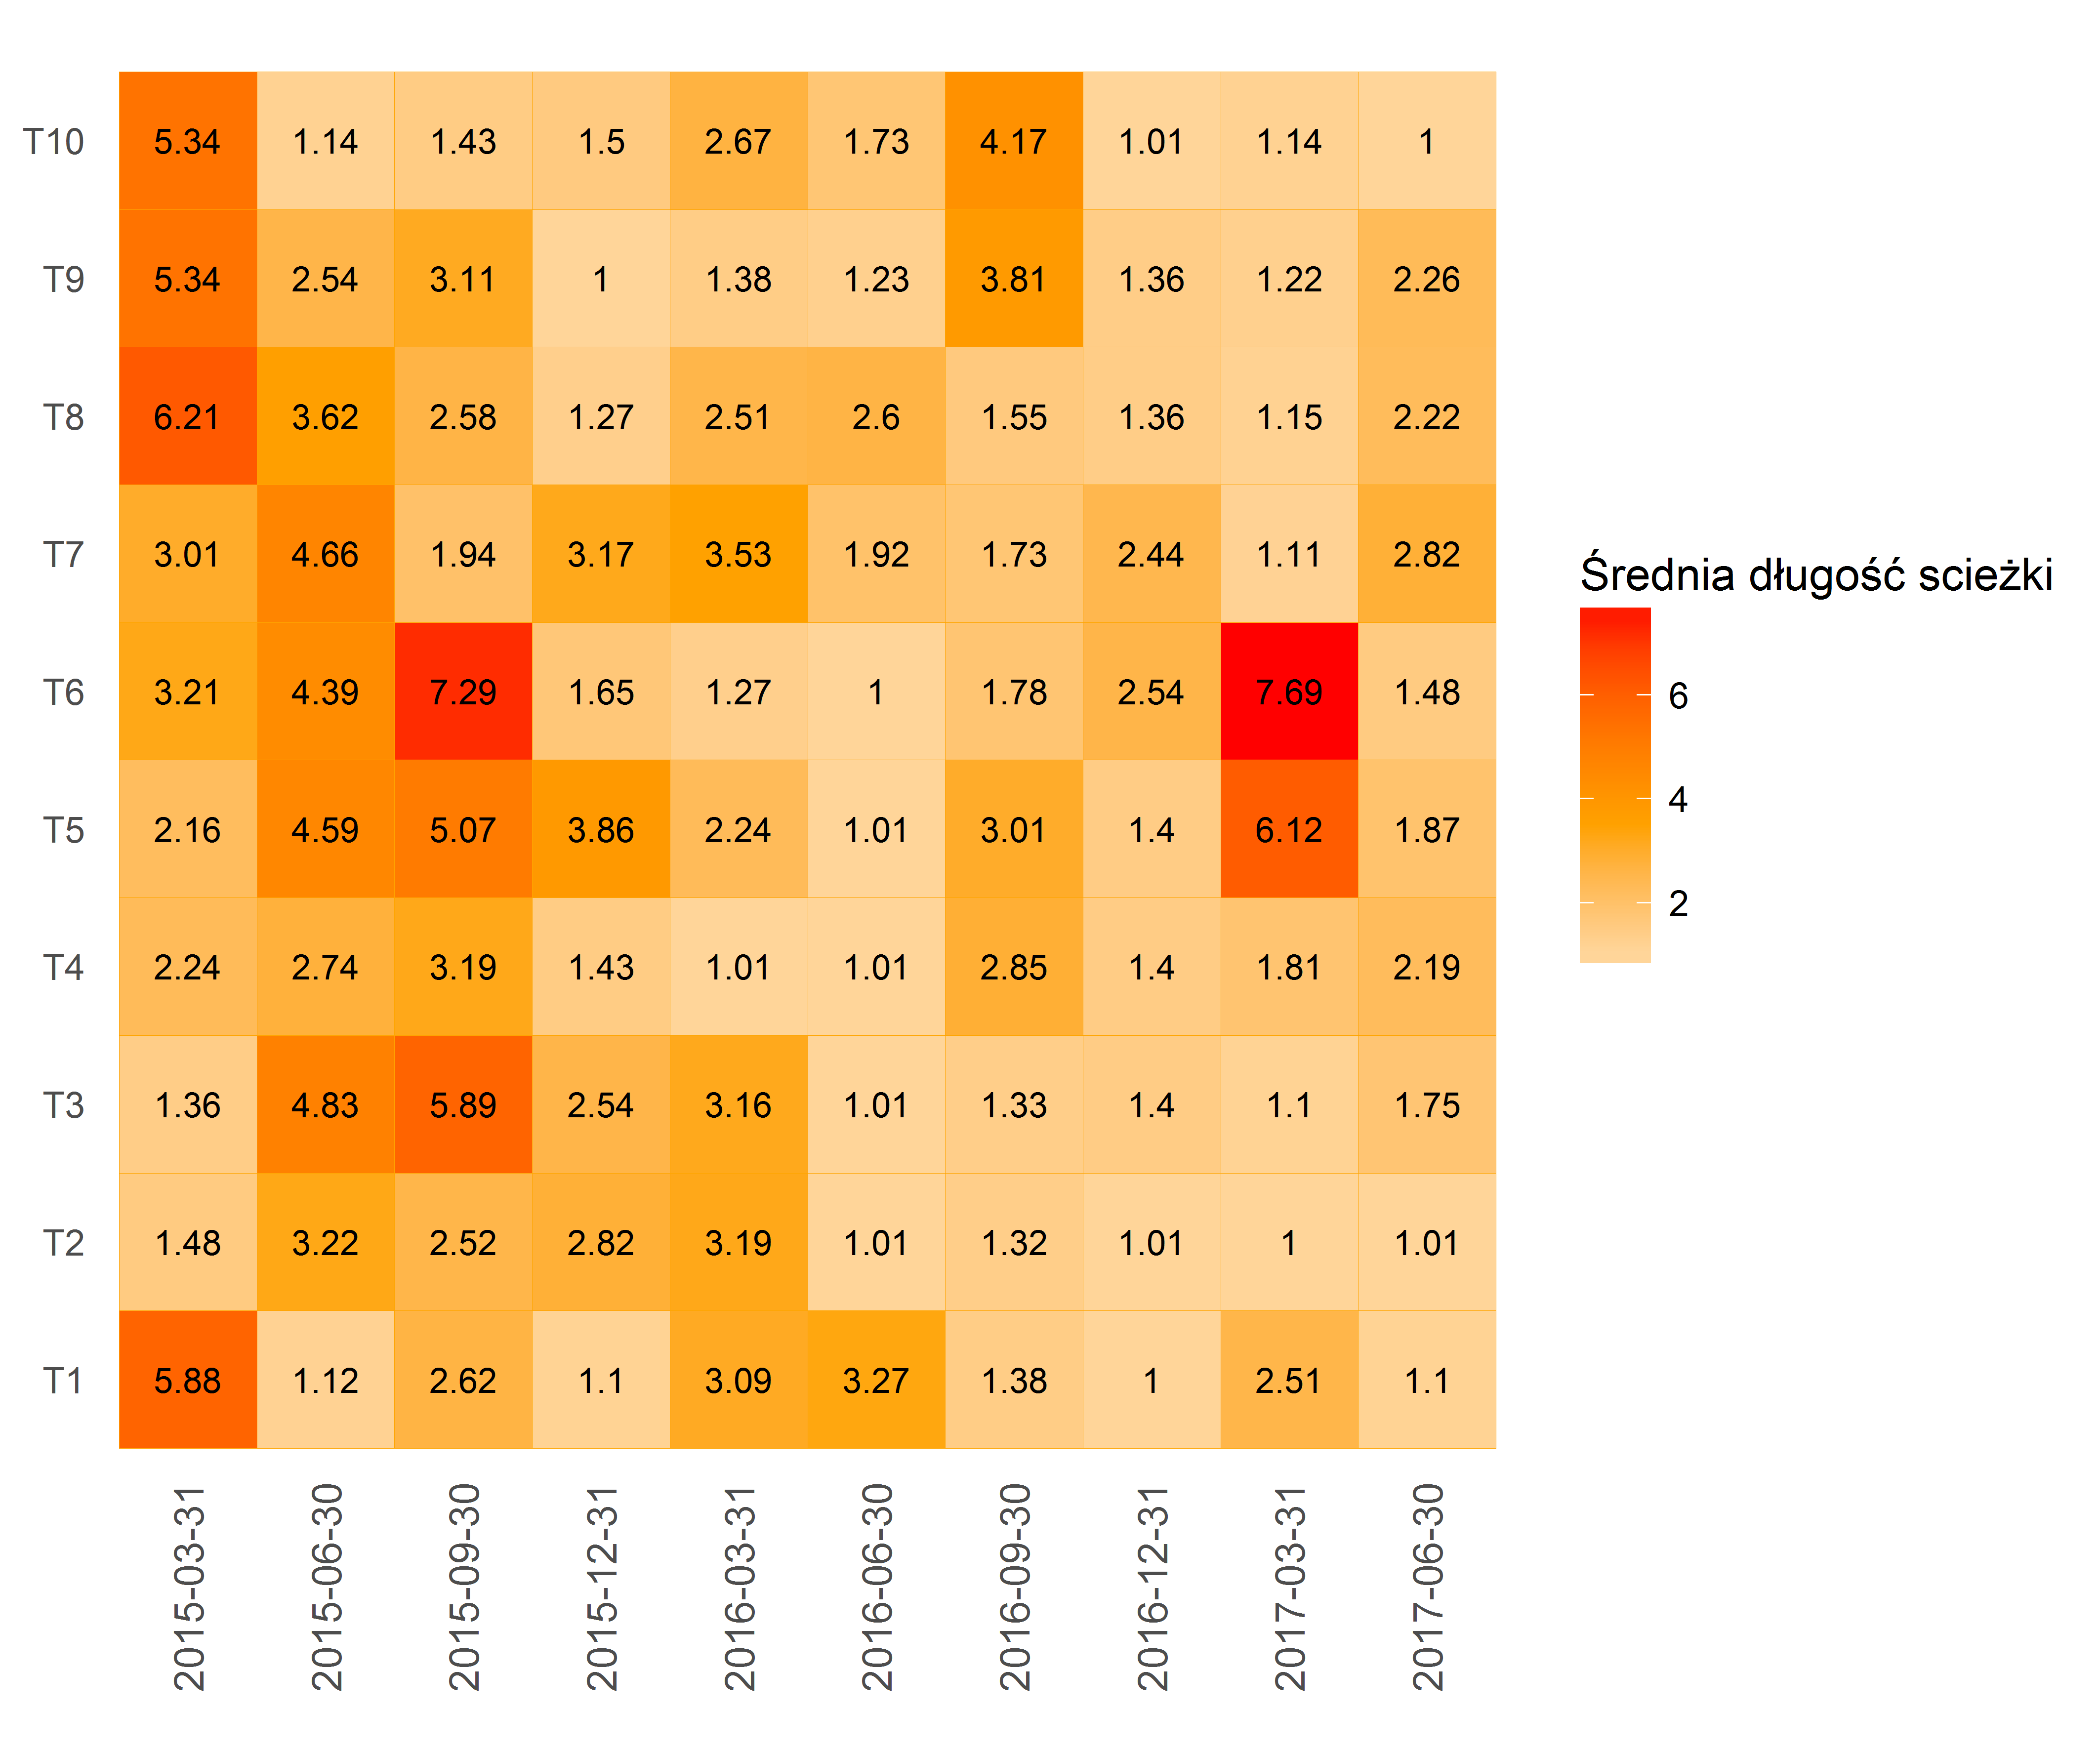
\includegraphics[width=0.9\linewidth]{pictures/srednia_dlugosc_sciezki/srednia_dlugosc_sciezki_hm.png}
  \caption{Mapa cieplna średniej długości scieżki w sieci dla 10 transakcji w 10 okresach.}
  \label{fig:sds1}
\end{figure}

\begin{figure}[H]
\centering
  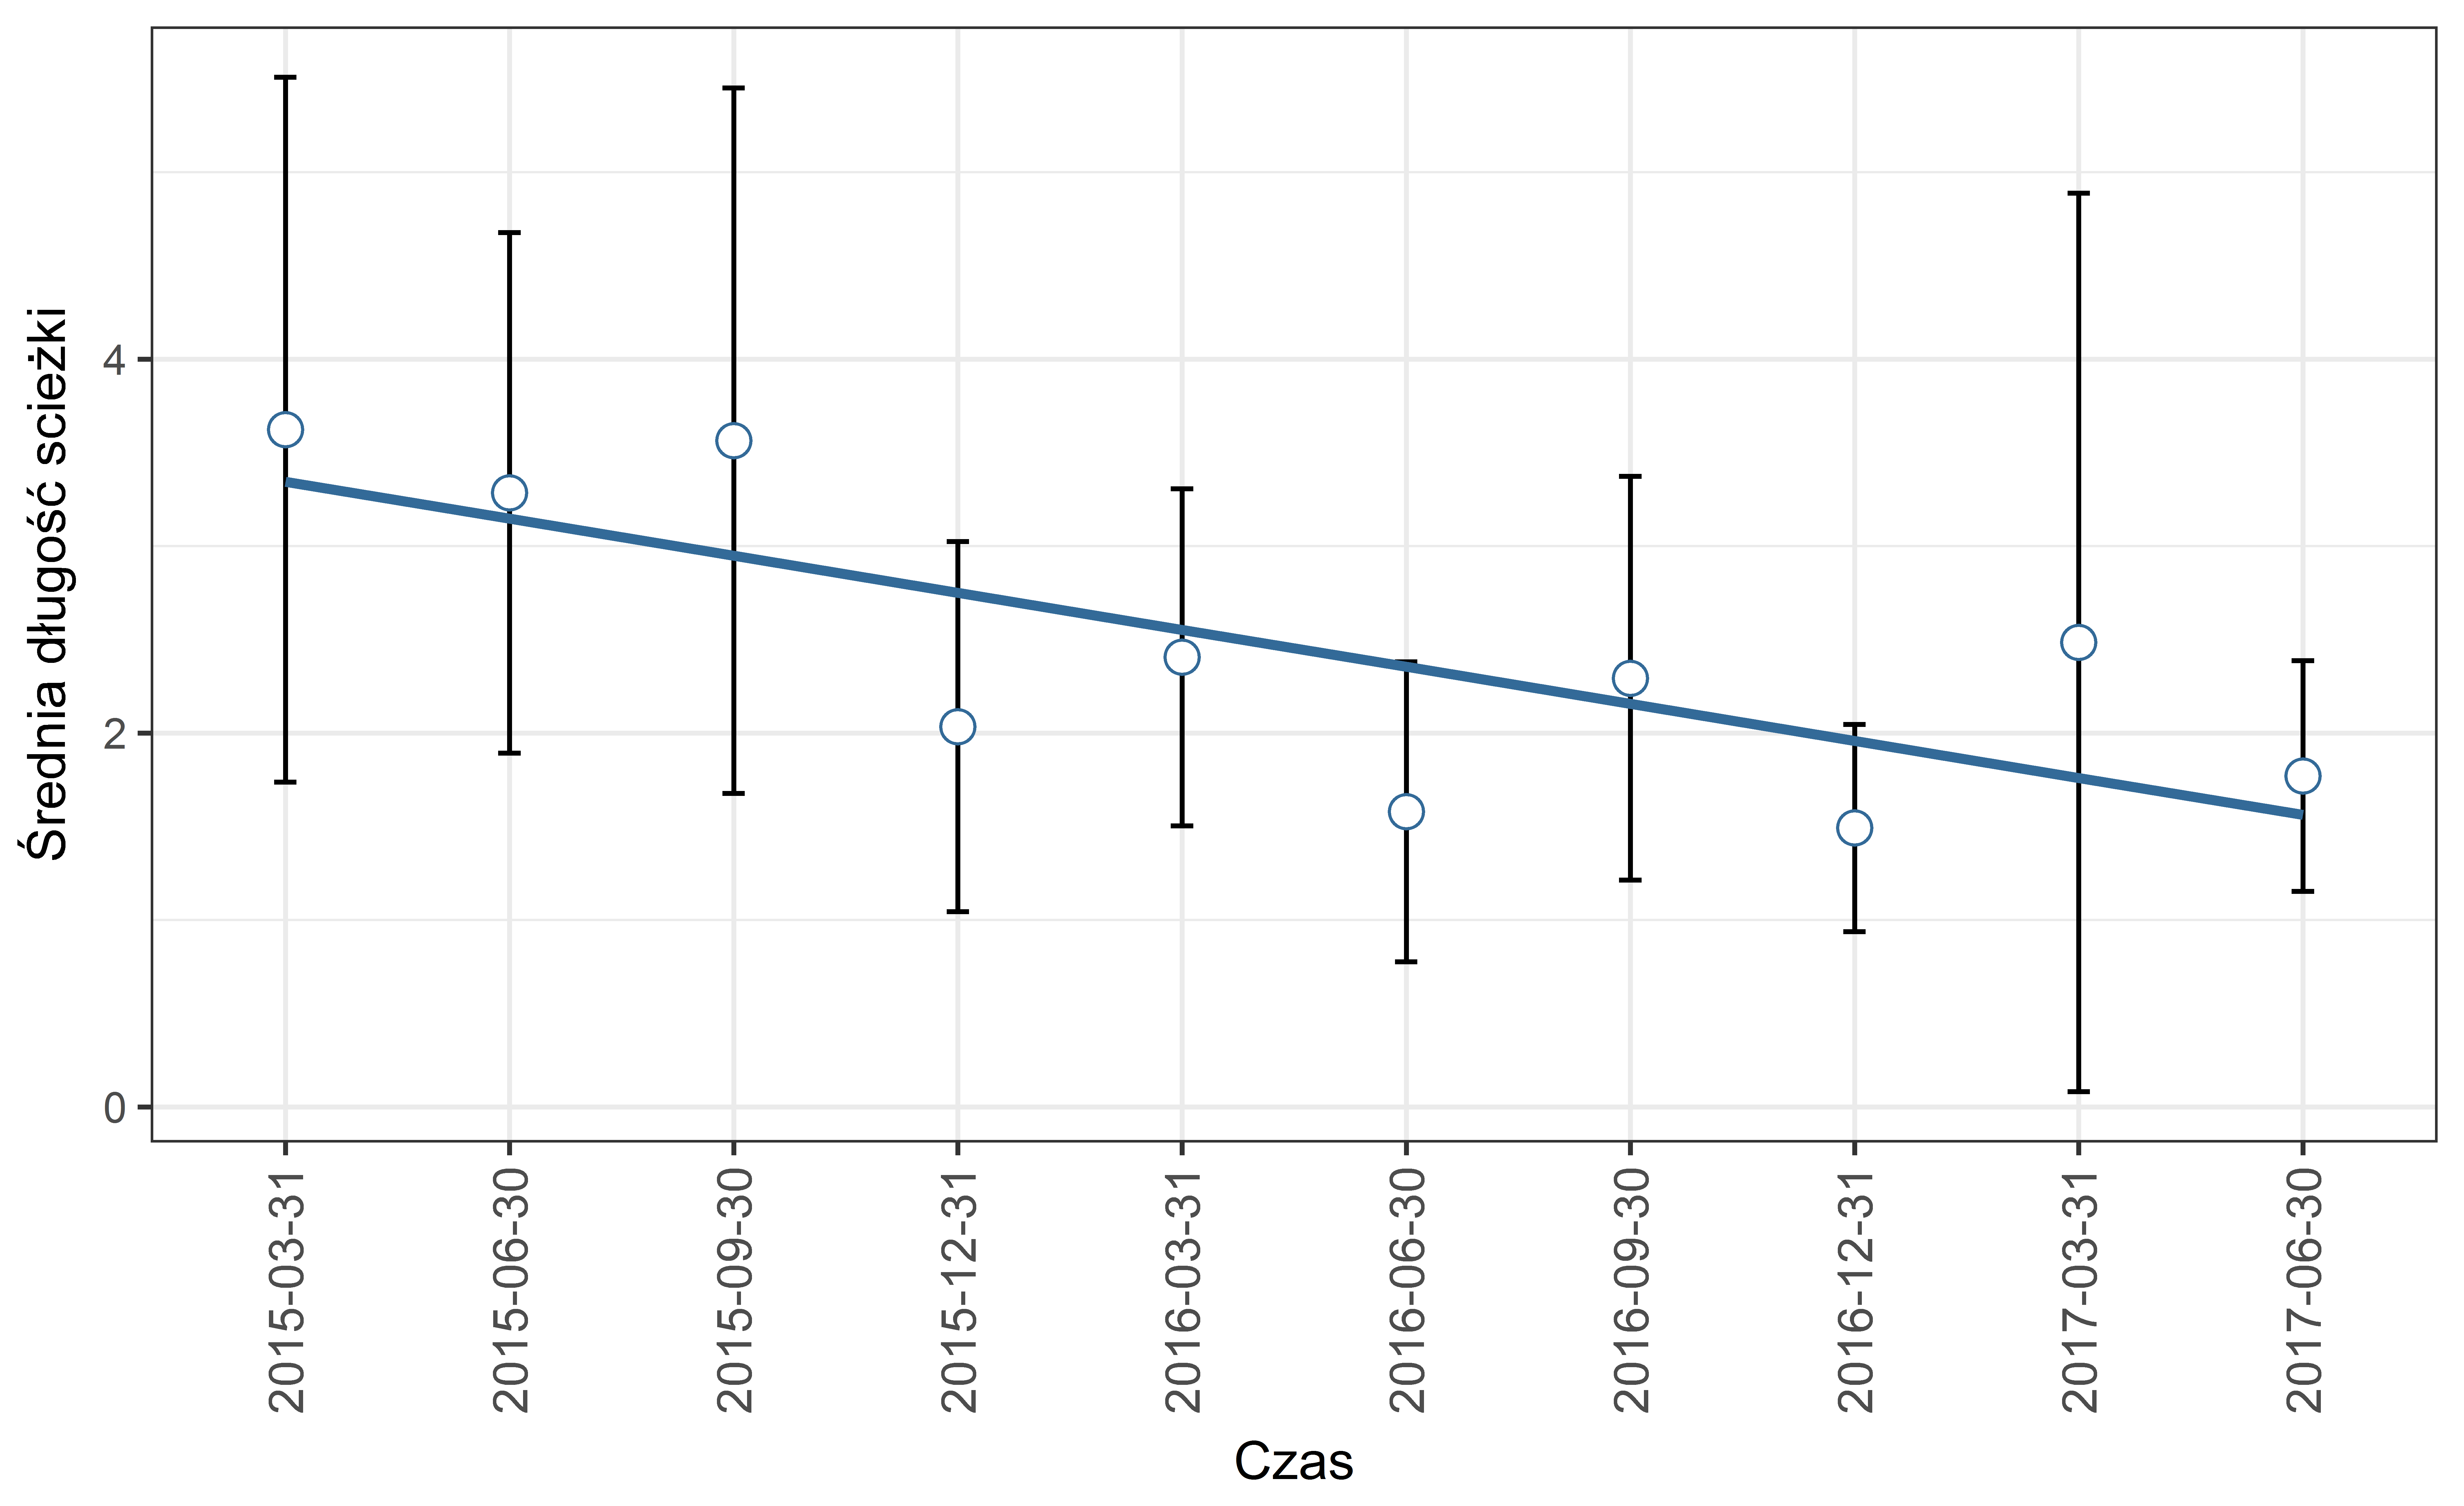
\includegraphics[width=0.9\linewidth]{pictures/srednia_dlugosc_sciezki/srednia_dlugosc_sciezki_sda.png}
  \caption{Regresja liniowa średniej długości scieżki sieci dla 10 okresów z odchyleniem standardowym.}
  \label{fig:sds2}
\end{figure}

\subsection{Badanie średniego stopnia węzła}

\indent Stopień węzła $v$ grafu oznacza liczbę krawędzi w grafie, które bezpośrednio dotykają węzła $v$. W grafach skierowanych wyróżnia się wejściowy stopień węzła (ilość krawędzi skierowanych w stronę węzła) oraz wyjściowy stopień węzła (ilość krawędzi skierowanych od strony węzła). Suma wejściowego stopnia węzła oraz wyjściowego stopnia wejścia daje wynikowy stopień węzła. Średni stopień węzła obliczany jest jako $\frac{\sum_i^n\deg(v_i)}{n}$, gdzie $deg(v_i)$ to stopień i-tego węzła, a $n$ to ilość węzłów. W celu zmniejszenia popełnienia błędu podczas interpretacji autentyczności obliczanej średniej badana próba powinna mieć rozkład normalny. W przeciwnym przypadku należy przedstawić dodatkowe źródło informacji o próbie, które zobrazuje częstotliwość występowania poszczególnych wartości, np. histogram. 

\indent W trakcie budowania sieci procesowanie każdej pojedynczej transakcji polega na sprawdzeniu jej adresów wyjściowych z adresami wejściowymi każdej transakcji do tej pory dołączonej do sieci. W przypadku wykrycia tego samego adresu w tych dwóch zbiorach adresów transakcji powstaje krawędź, która je łączy. W przypadku badania stopnia węzła transakcji w łańcucha transakcji sieci bitcoin określana jest ilość transakcji, z którymi dana transakcja dzieli adres w danej próbce. 


%\begin{figure}
%\centering
%
%\begin{subfigure}[b]{0.85\textwidth}
%   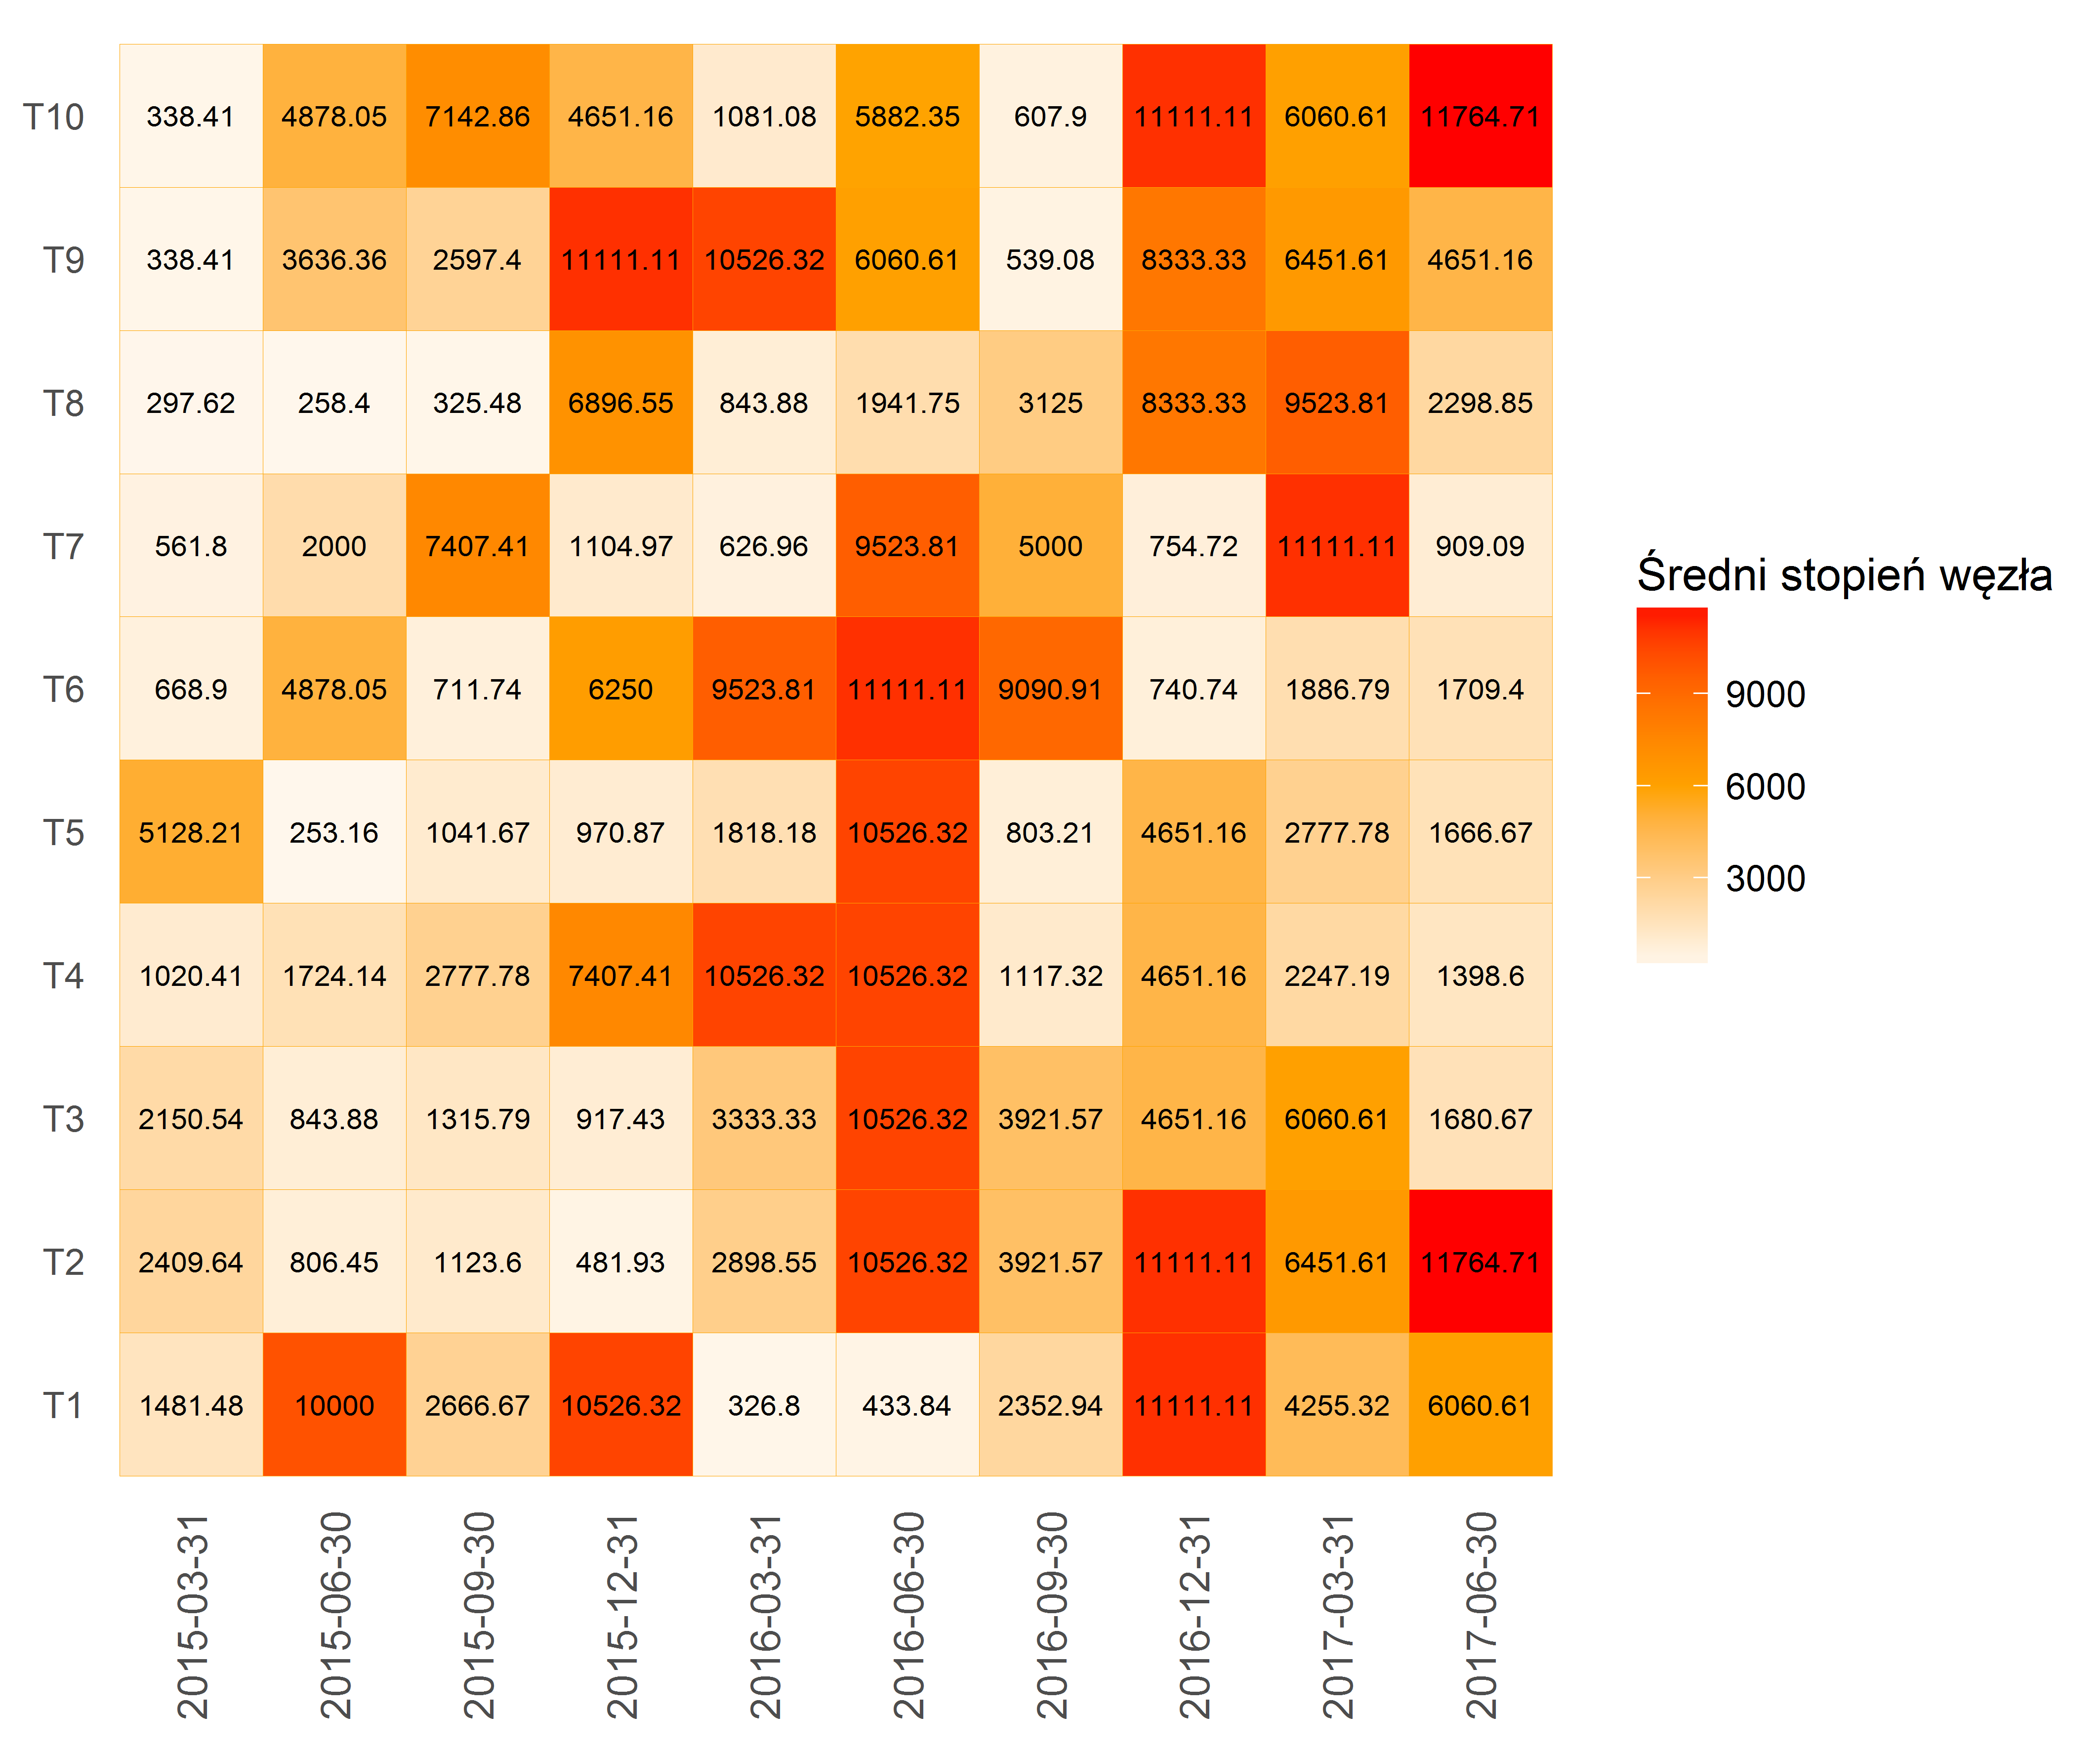
\includegraphics[width=1\linewidth]{pictures/sredni_stopien_wezla/sredni_stopien_wezla_hm.png}
%   \caption{}
%   \label{fig:sw1} 
%\end{subfigure}
%
%\begin{subfigure}[b]{0.85\textwidth}
%   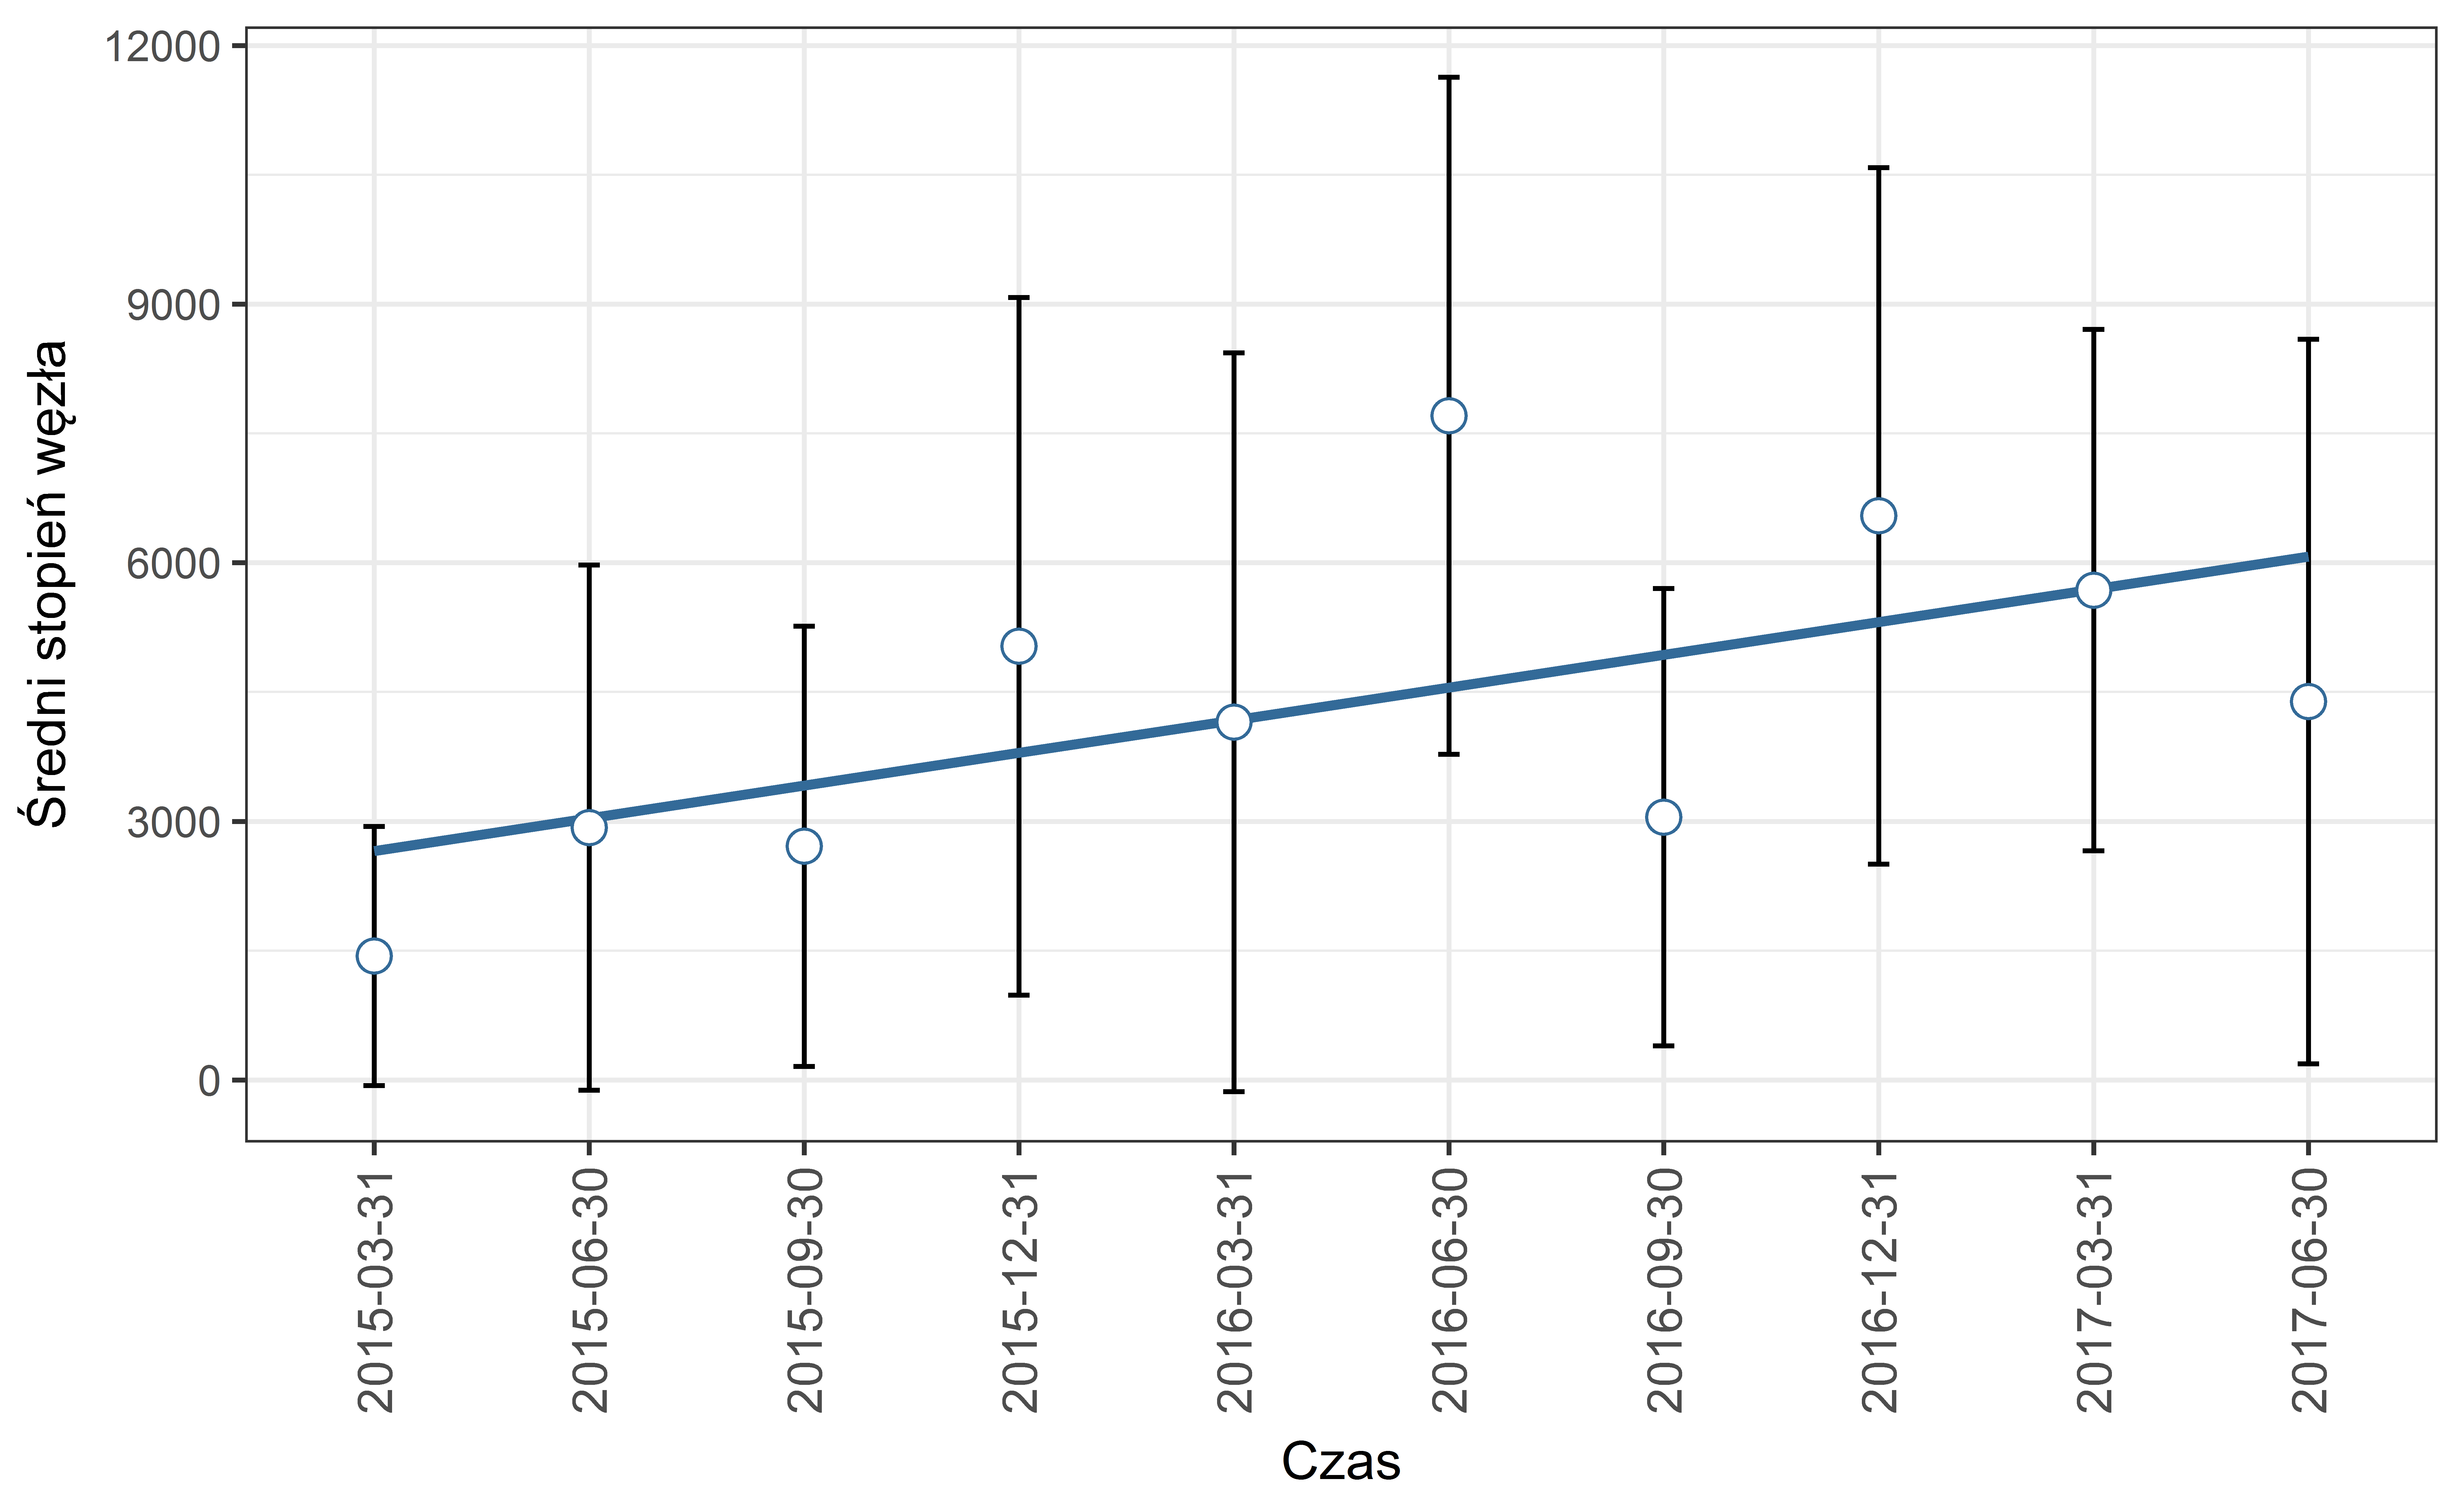
\includegraphics[width=1\linewidth]{pictures/sredni_stopien_wezla/sredni_stopien_wezla_sda.png}
%   \caption{}
%   \label{fig:sw2}
%\end{subfigure}
%
%\begin{subfigure}[b]{0.85\textwidth}
%   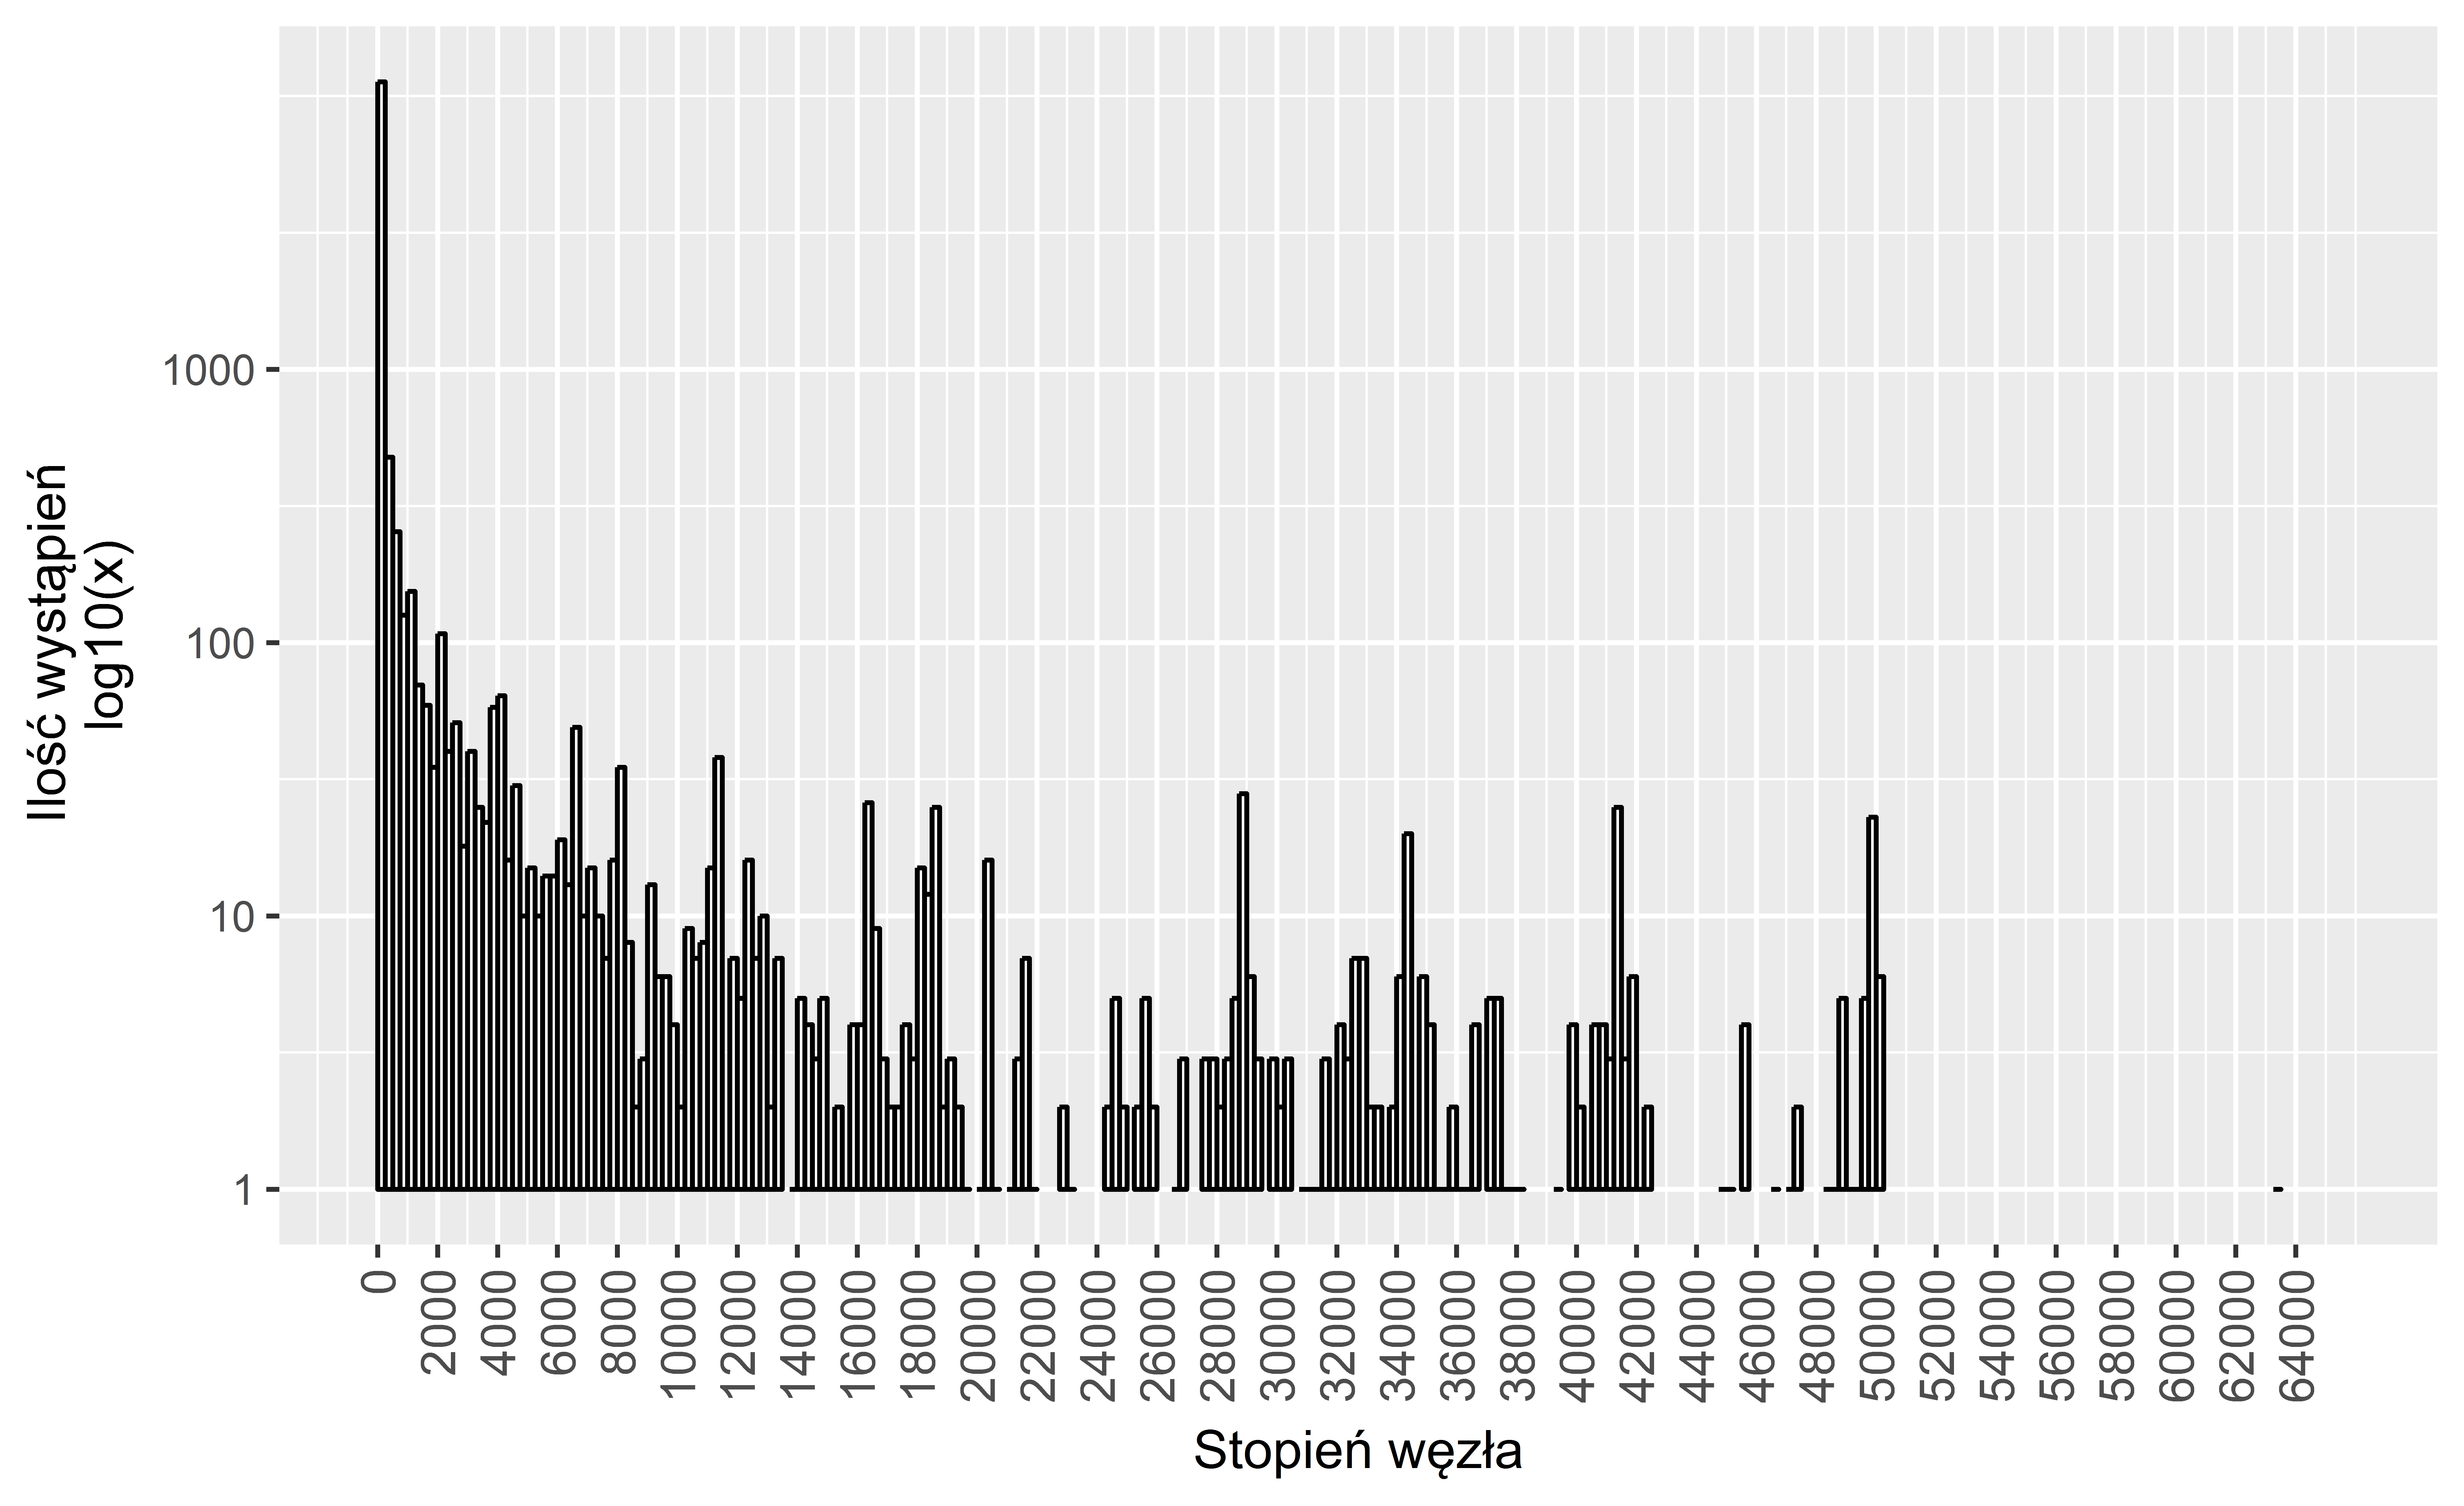
\includegraphics[width=1\linewidth]{pictures/sredni_stopien_wezla/sredni_stopien_wezla_hist.png}
%   \caption{}
%   \label{fig:sw3}
%\end{subfigure}
%
%\caption[Średni stopień węzła]{(a) mapa cieplna średniego stopnia węzła sieci dla 10 transakcji w 10 okresach (b) regresja liniowa średniego stopnia węzła sieci dla 10 okresów z odchyleniem standardowym (c) histogram średniego stopnia węzła sieci dla 10 transakcji w 10 okresach}
%
%\end{figure}
%
%
%\begin{figure}
%\centering
%
%\begin{subfigure}[b]{0.85\textwidth}
%   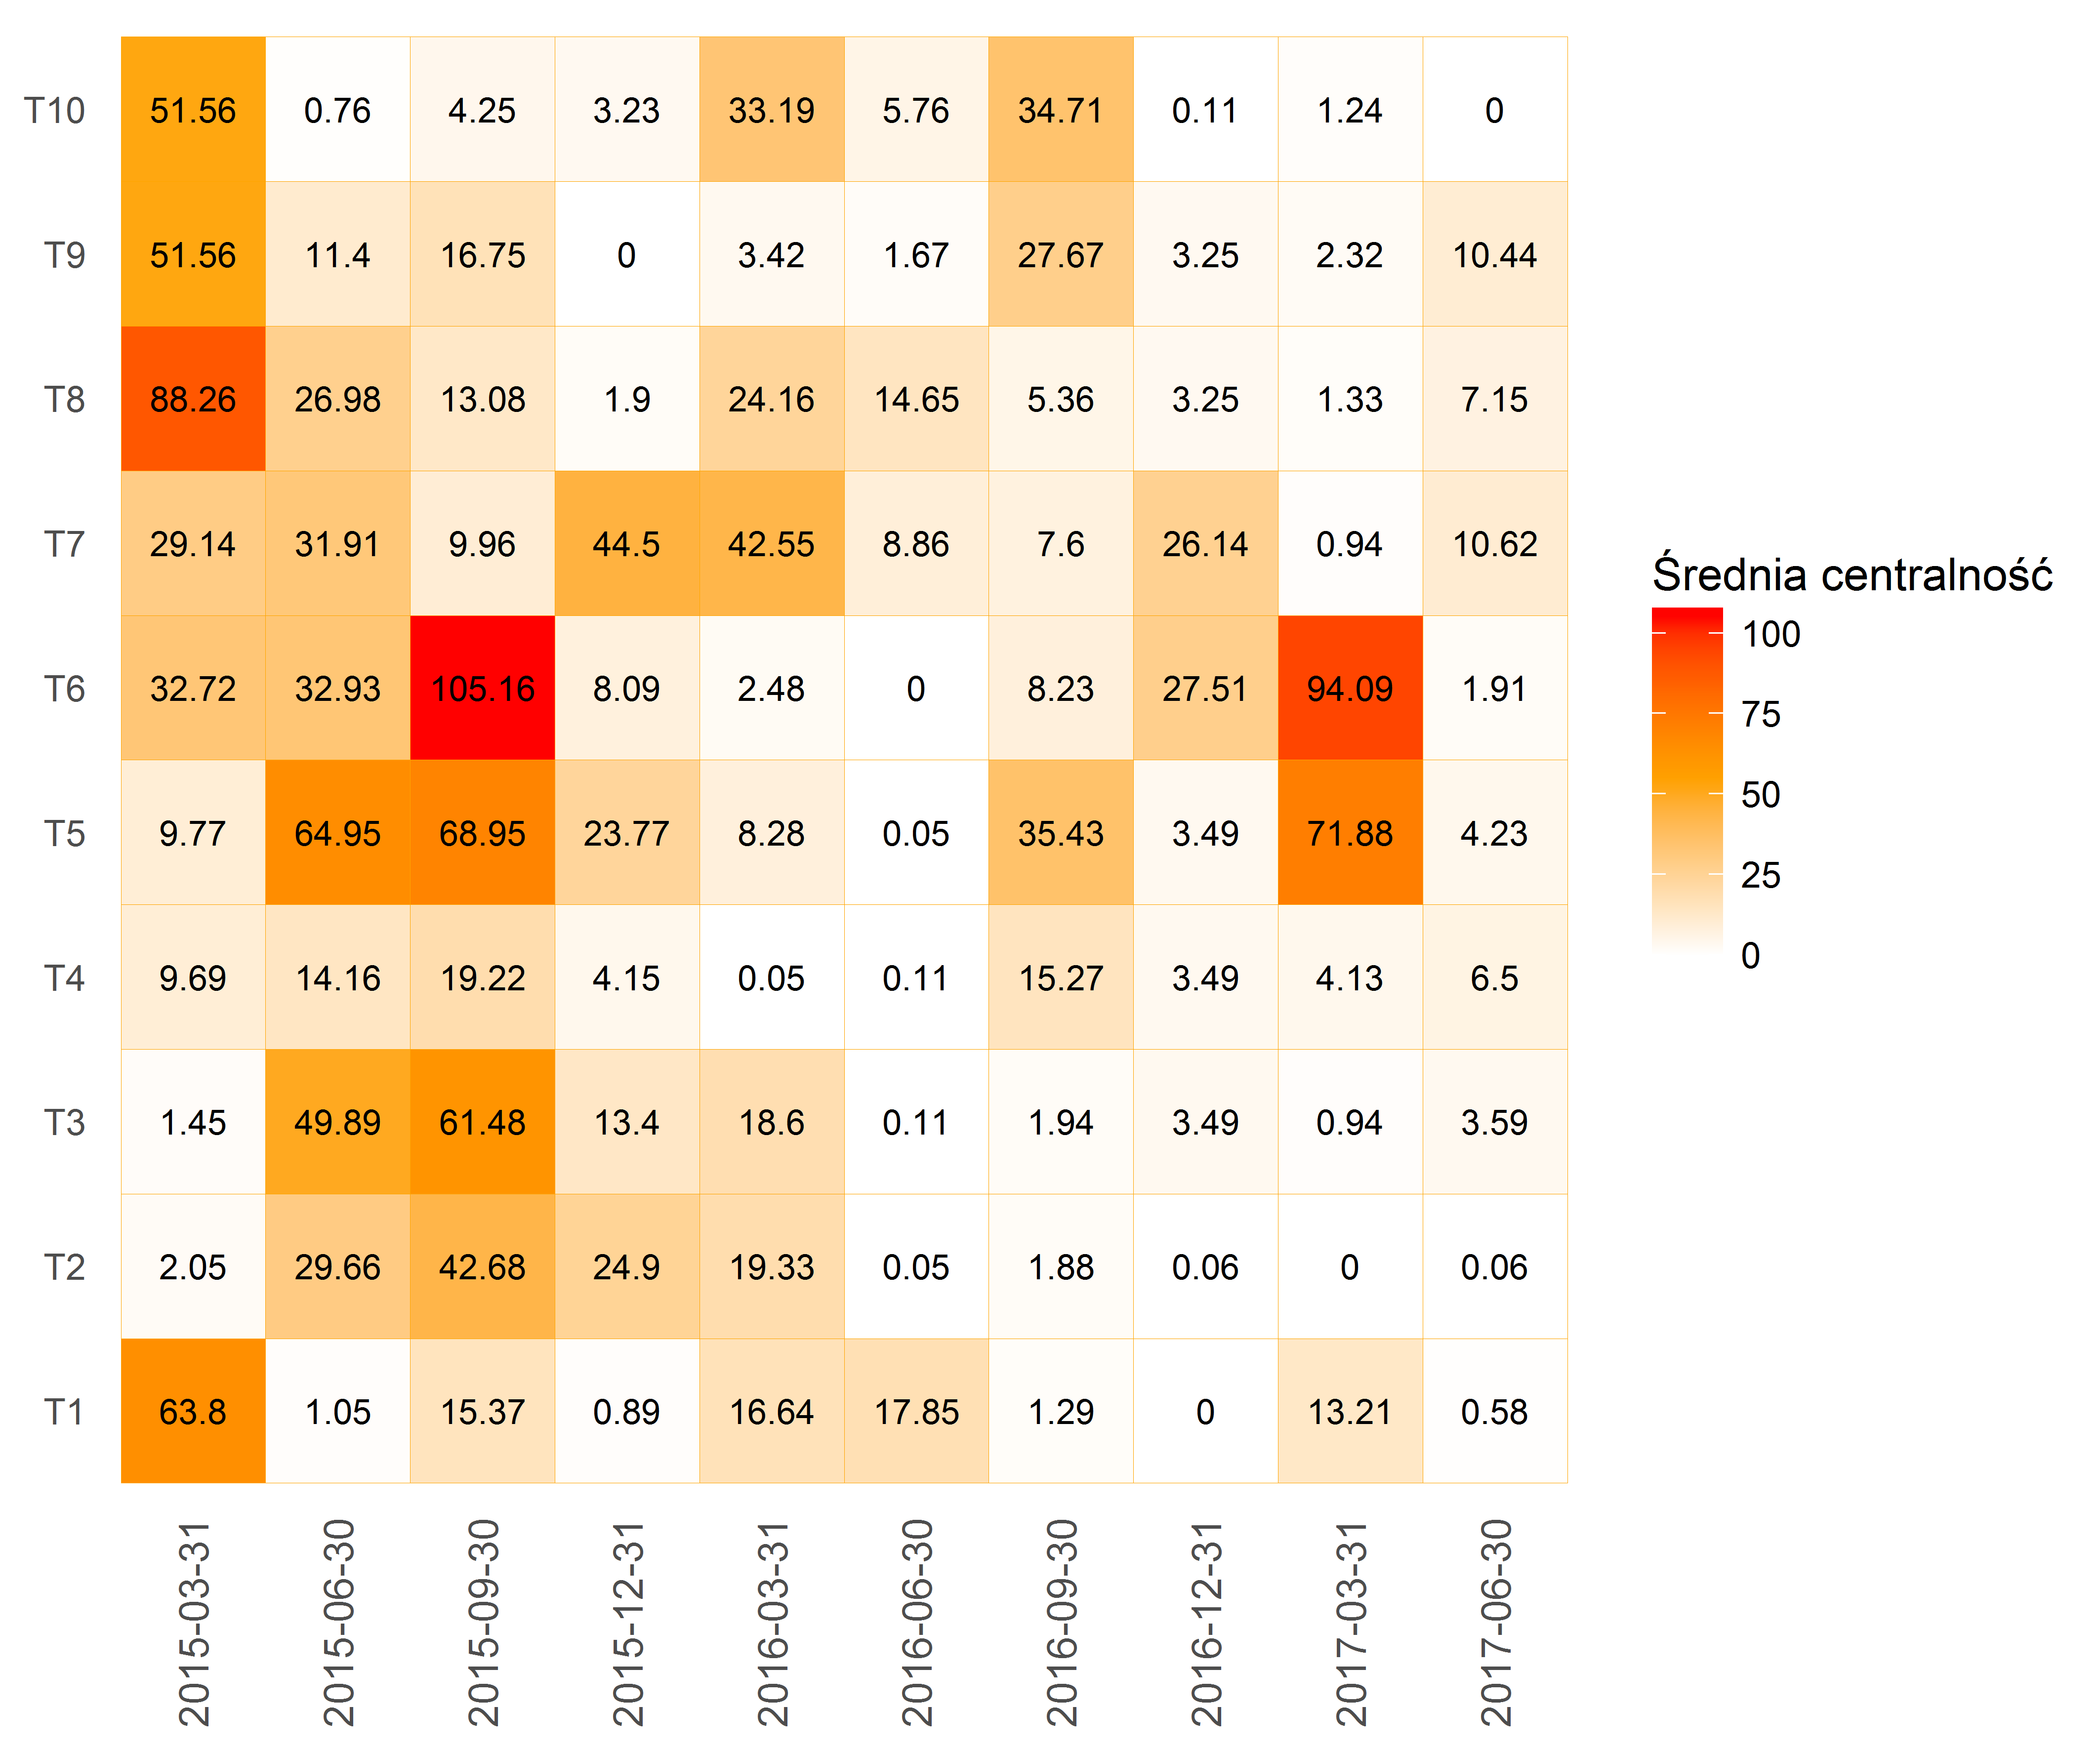
\includegraphics[width=1\linewidth]{pictures/srednia_centralnosc/srednia_centralnosc_hm.png}
%   \caption{}
%   \label{fig:sc1} 
%\end{subfigure}
%
%\begin{subfigure}[b]{0.85\textwidth}
%   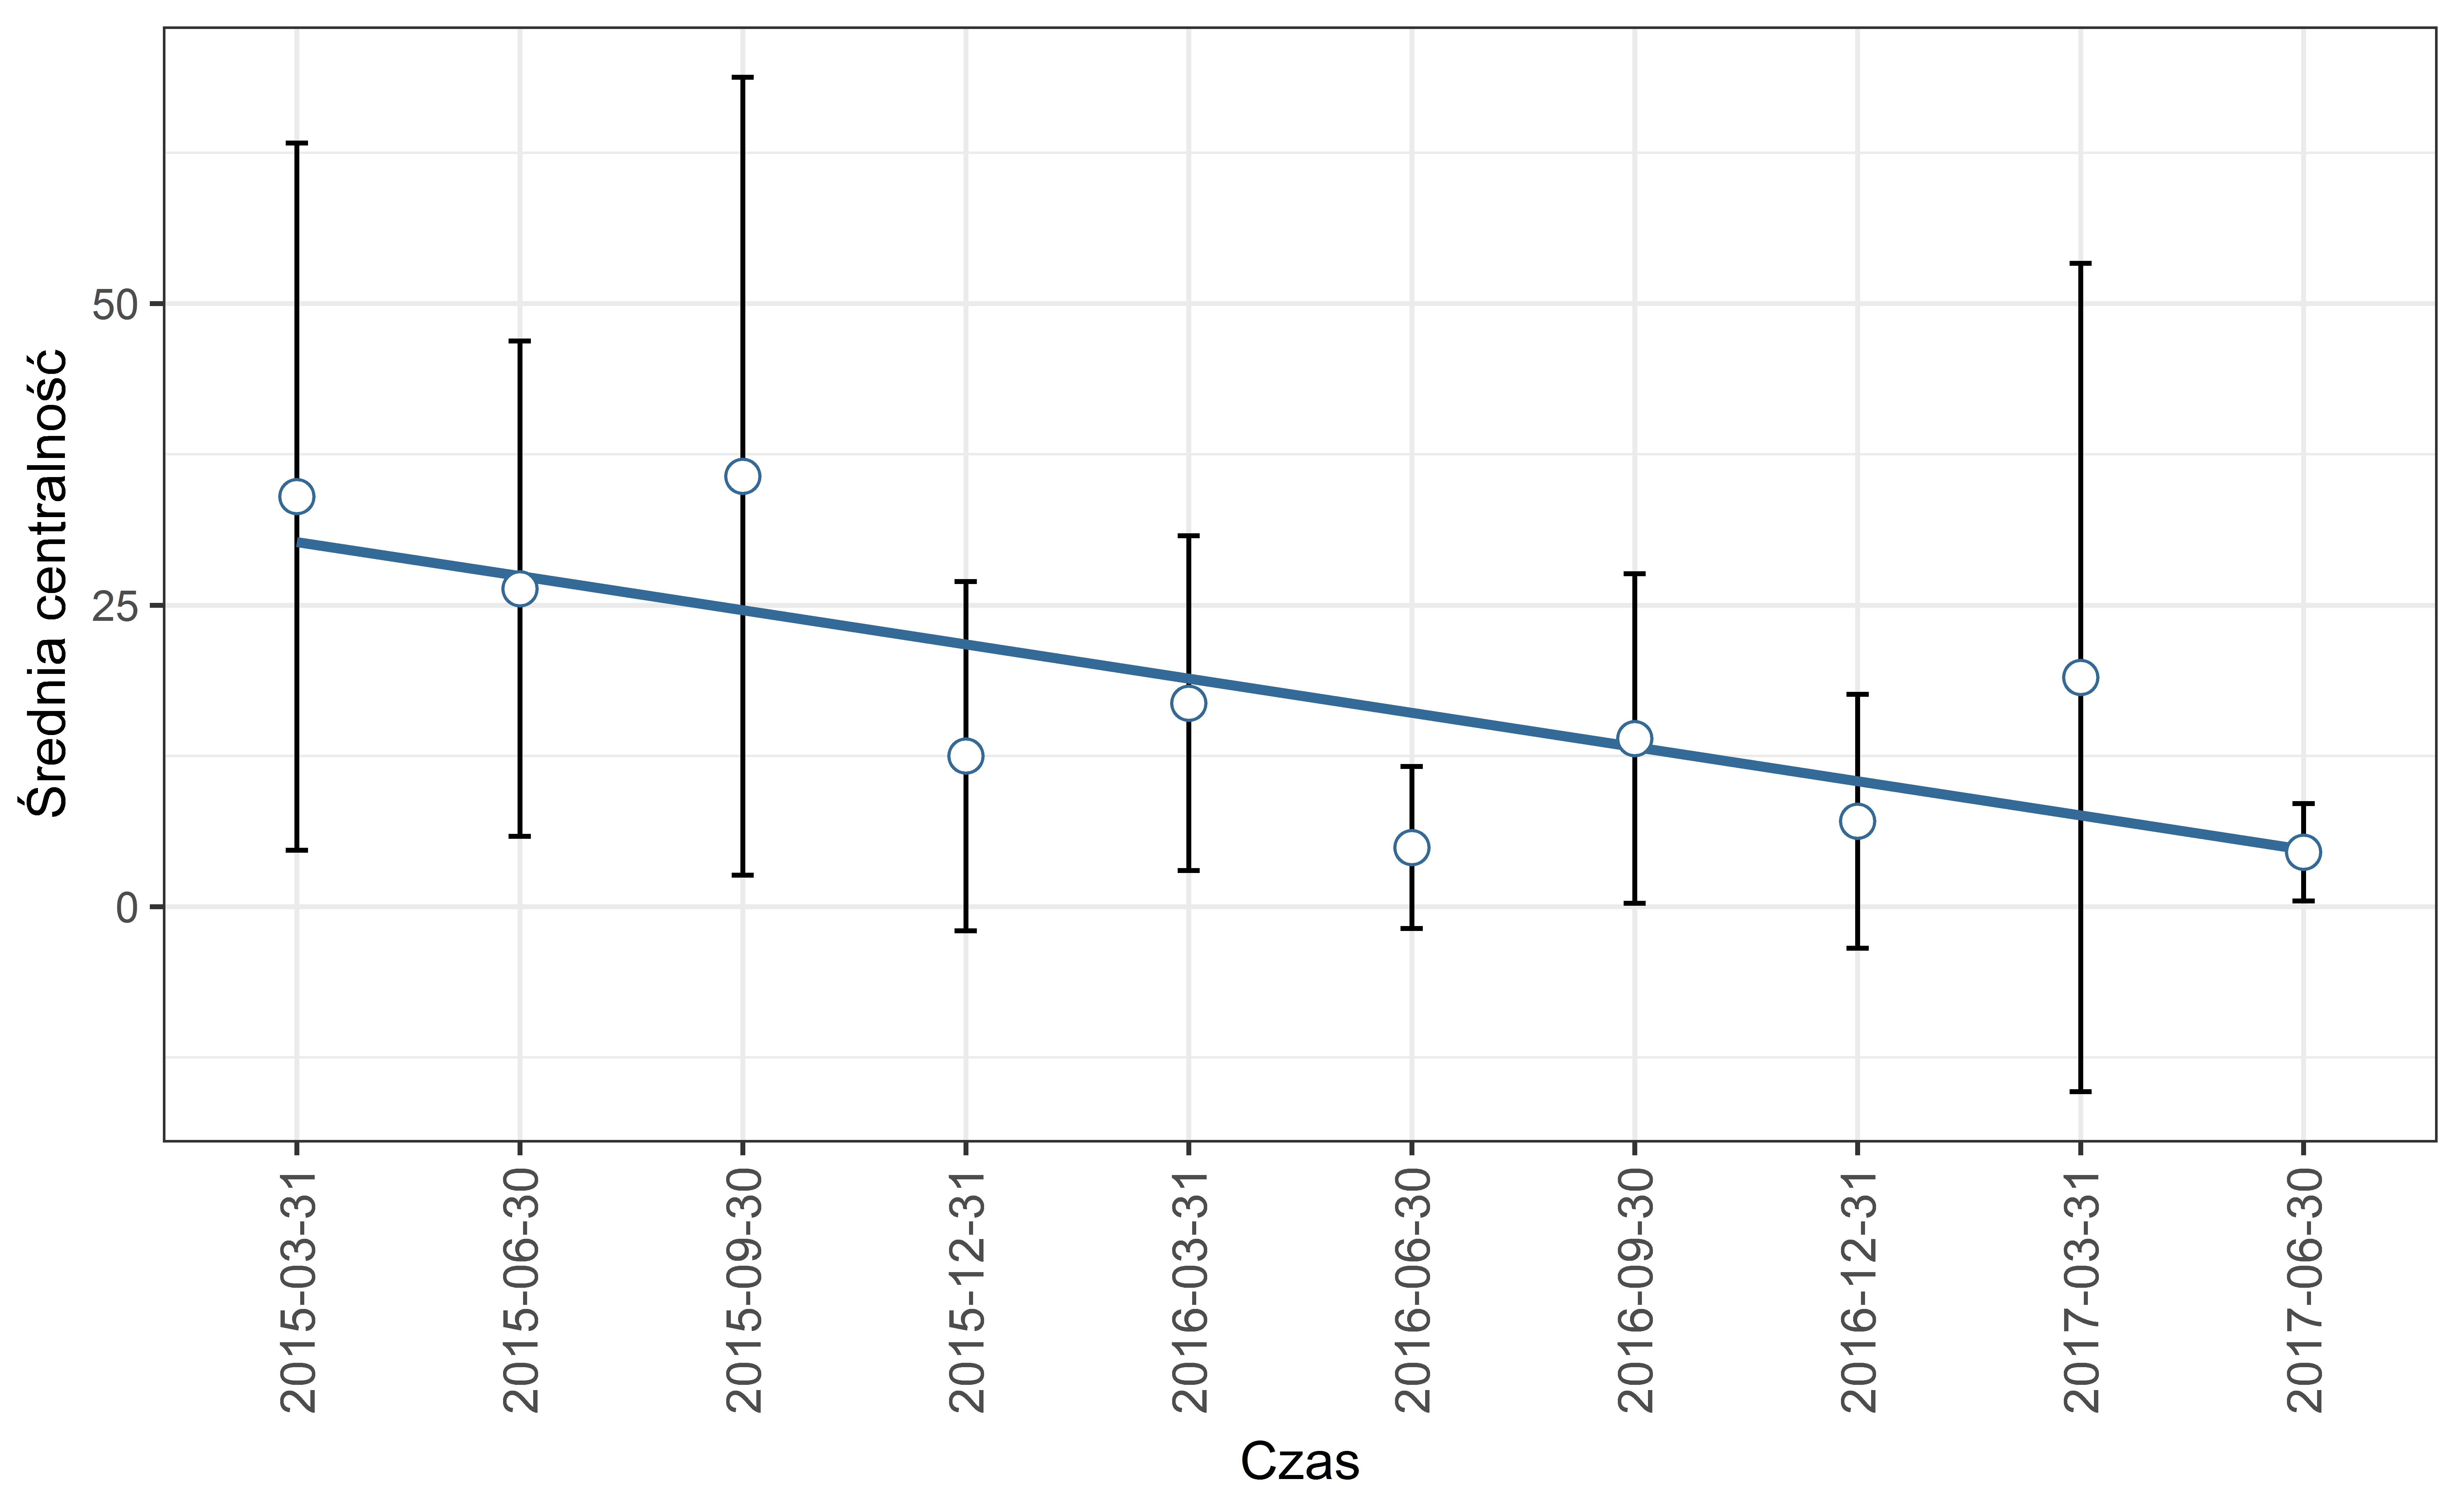
\includegraphics[width=1\linewidth]{pictures/srednia_centralnosc/srednia_centralnosc_sda.png}
%   \caption{}
%   \label{fig:sc2}
%\end{subfigure}
%
%\begin{subfigure}[b]{0.85\textwidth}
%   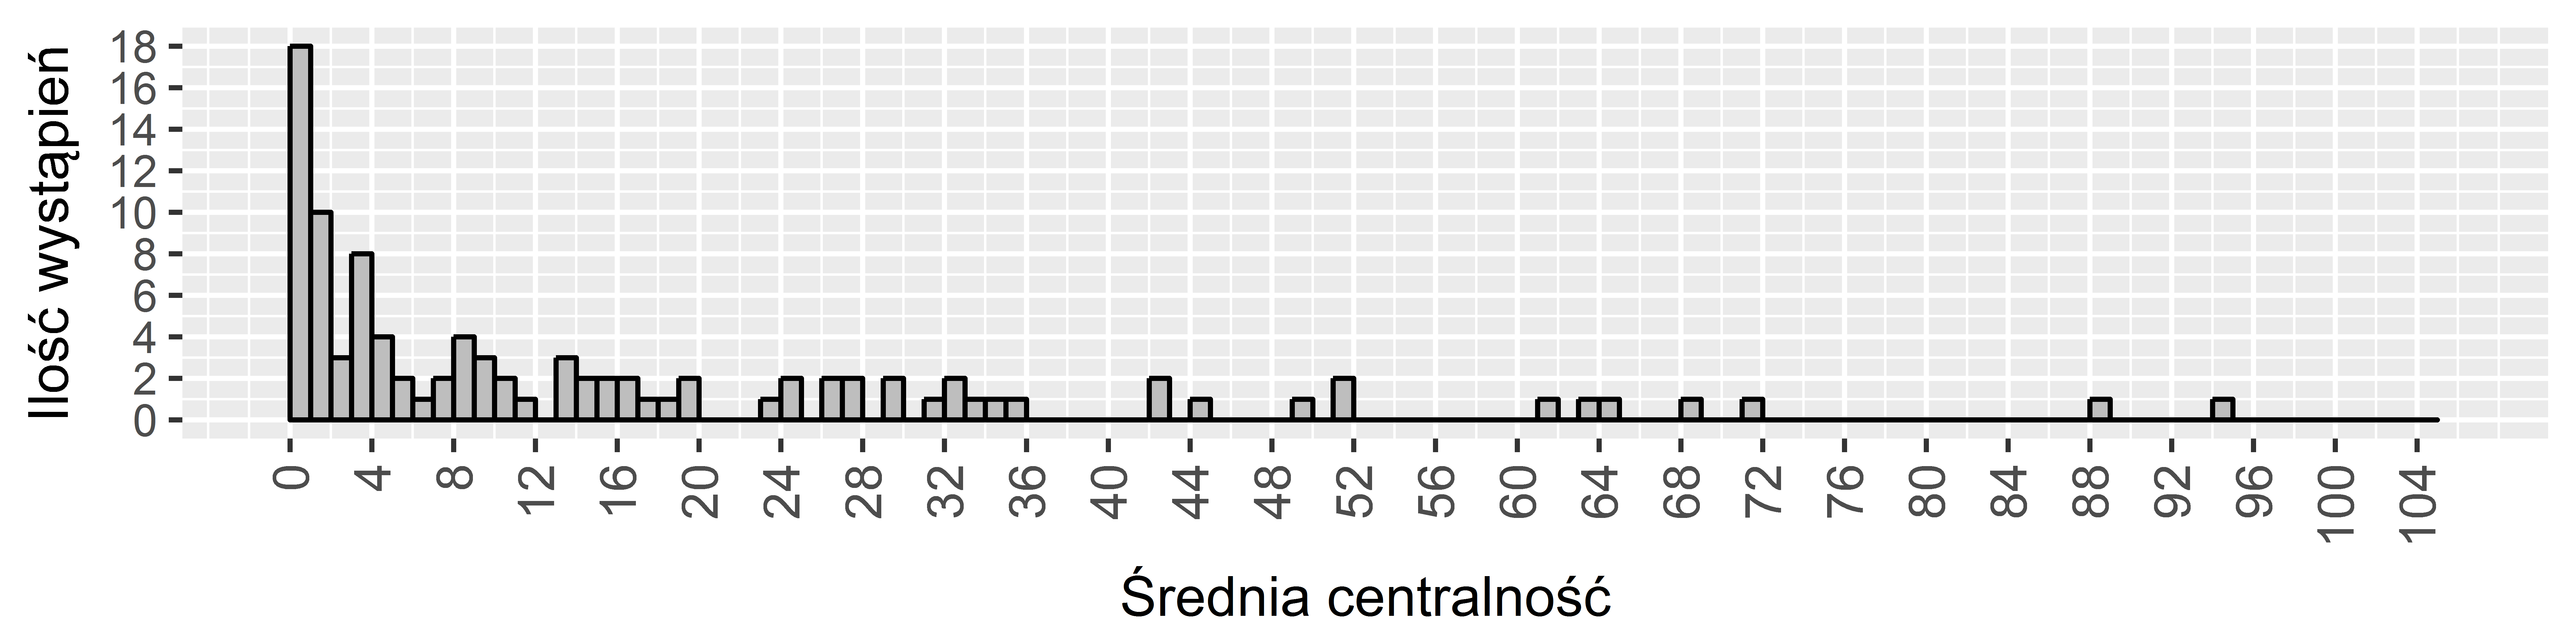
\includegraphics[width=1\linewidth]{pictures/srednia_centralnosc/srednia_centralnosc_hist.png}
%   \caption{}
%   \label{fig:sc3}
%\end{subfigure}
%
%\caption[Średnia centralność sieci]{(a) mapa cieplna średniej centralności sieci dla 10 transakcji w 10 okresach (b) regresja liniowa średniej centralności sieci dla 10 okresów z odchyleniem standardowym (c) histogram średniej centralności sieci dla 10 transakcji w 10 okresach}
%
%\end{figure}
%
%
%\begin{figure}
%\centering
%
%\begin{subfigure}[b]{0.85\textwidth}
%   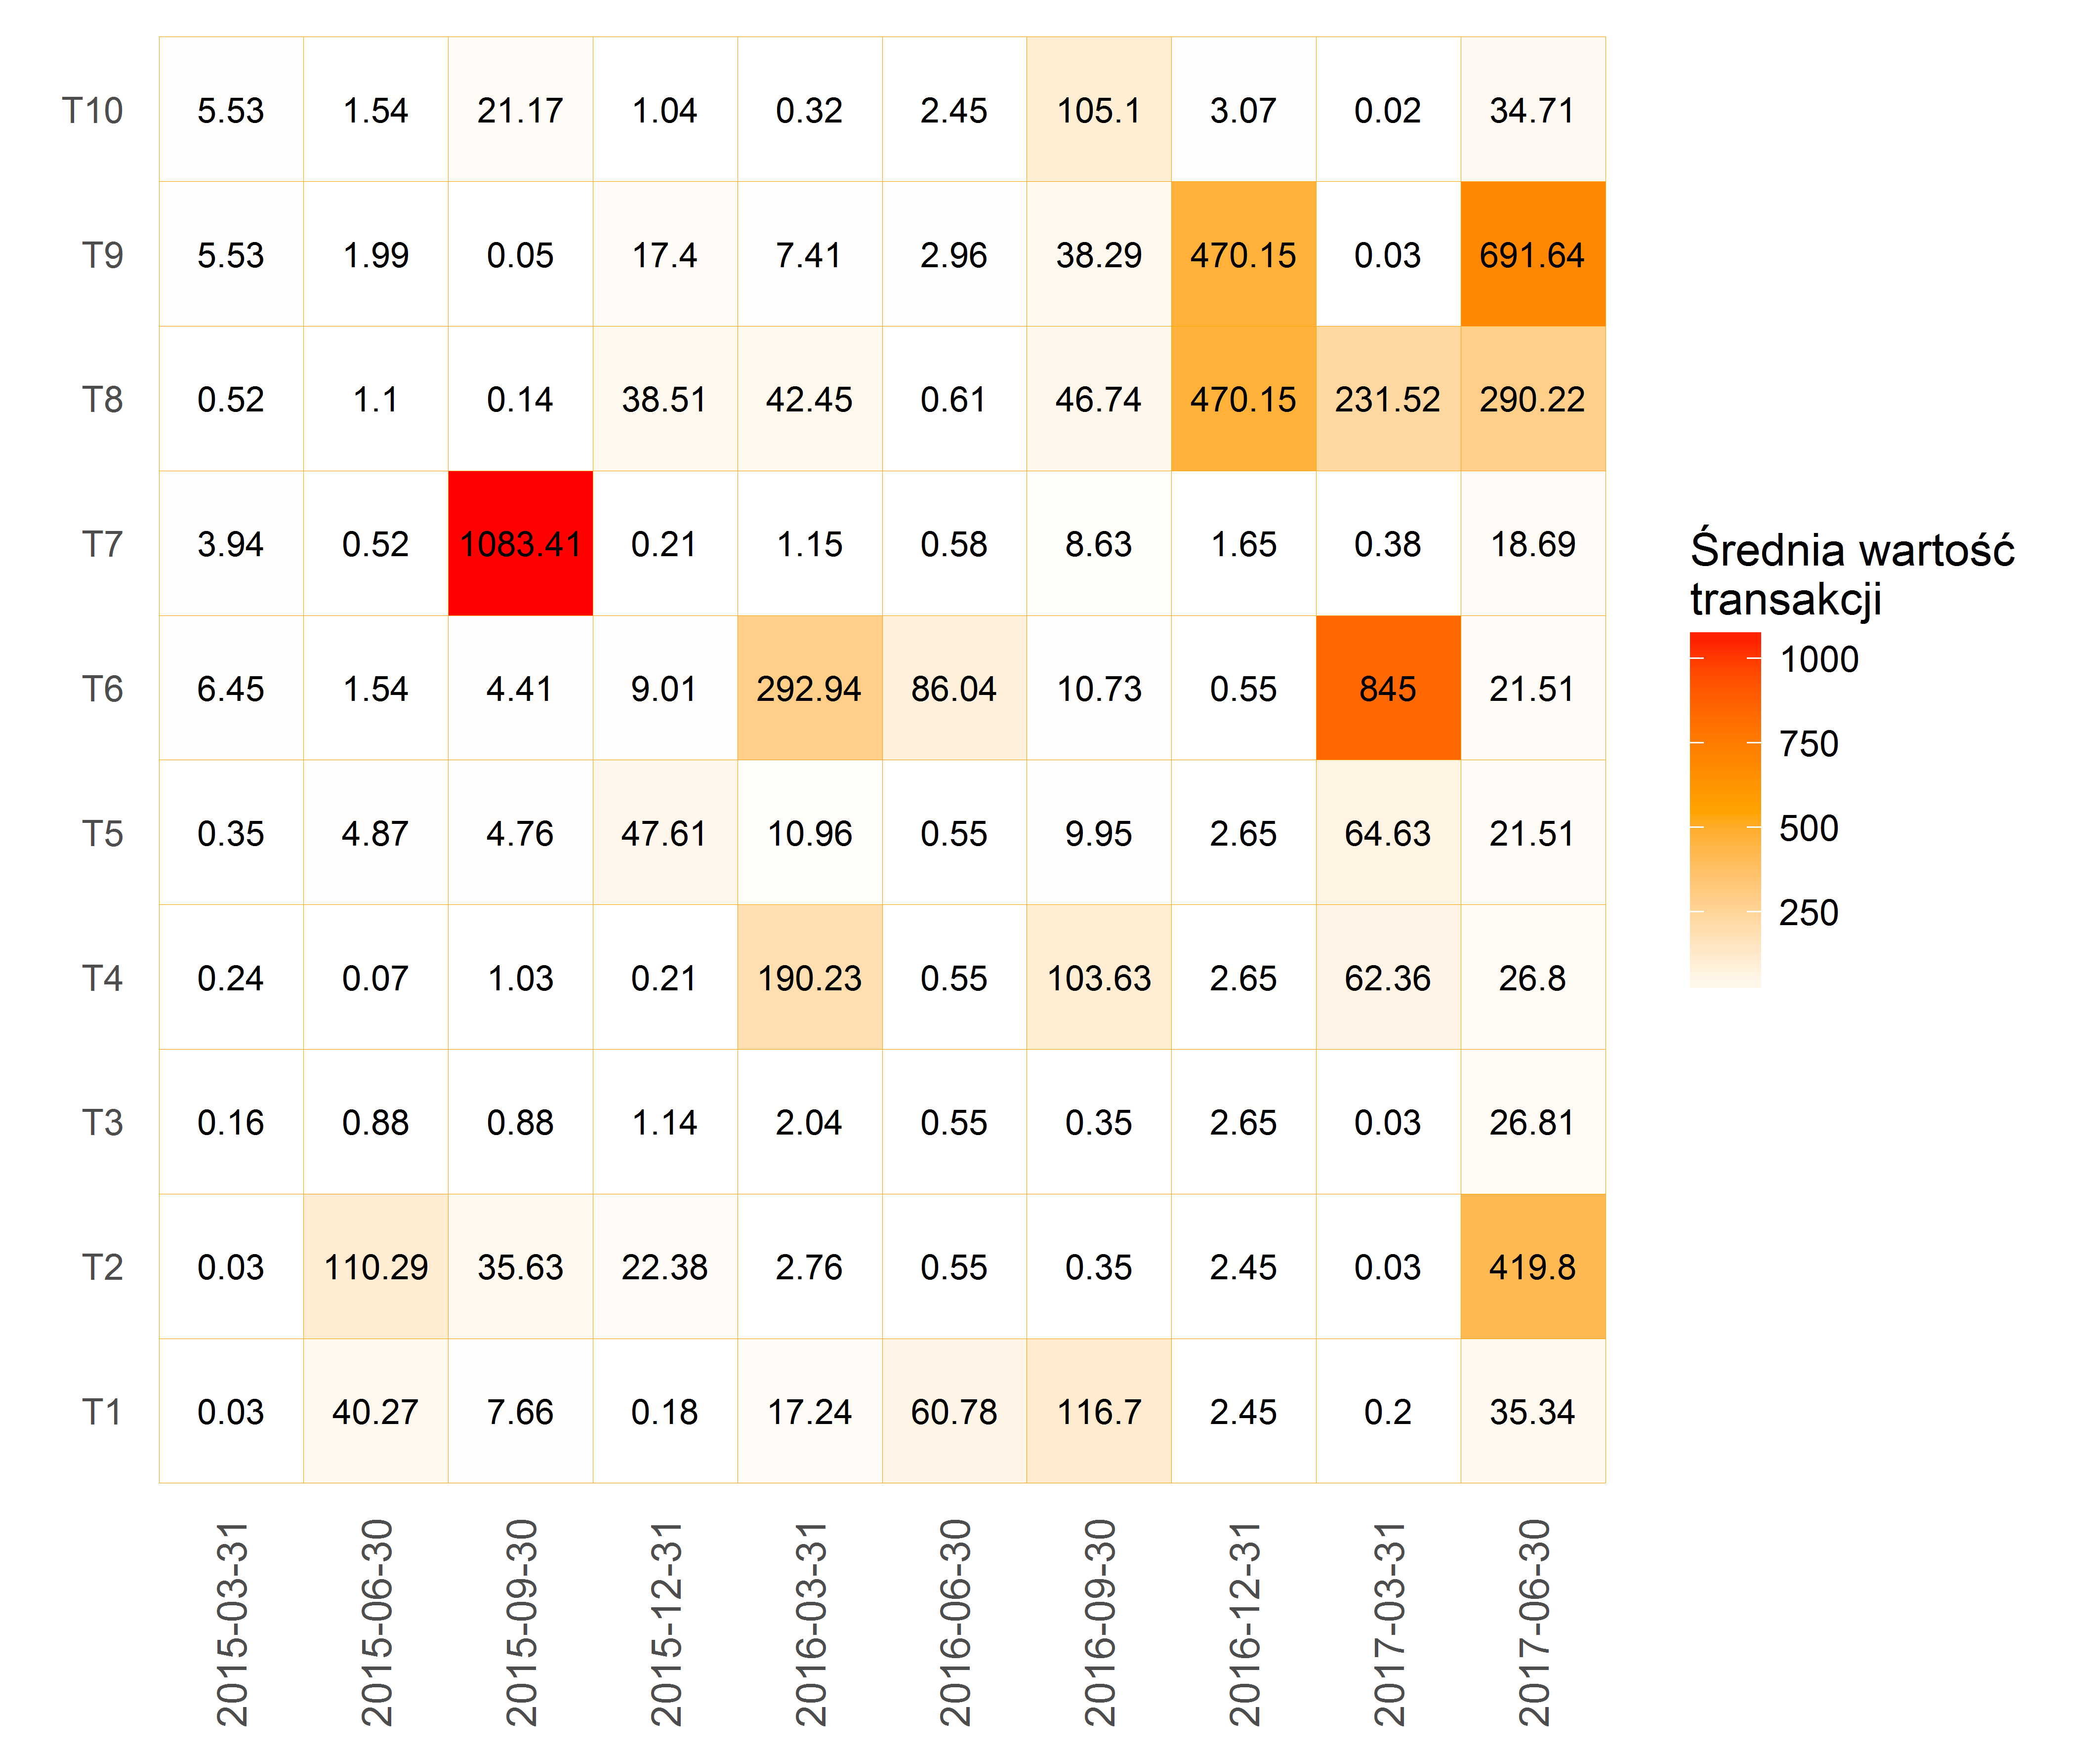
\includegraphics[width=1\linewidth]{pictures/wartosc_transakcji/wartosc_transakcji_hm.png}
%   \caption{}
%   \label{fig:wt1} 
%\end{subfigure}
%
%\begin{subfigure}[b]{0.85\textwidth}
%   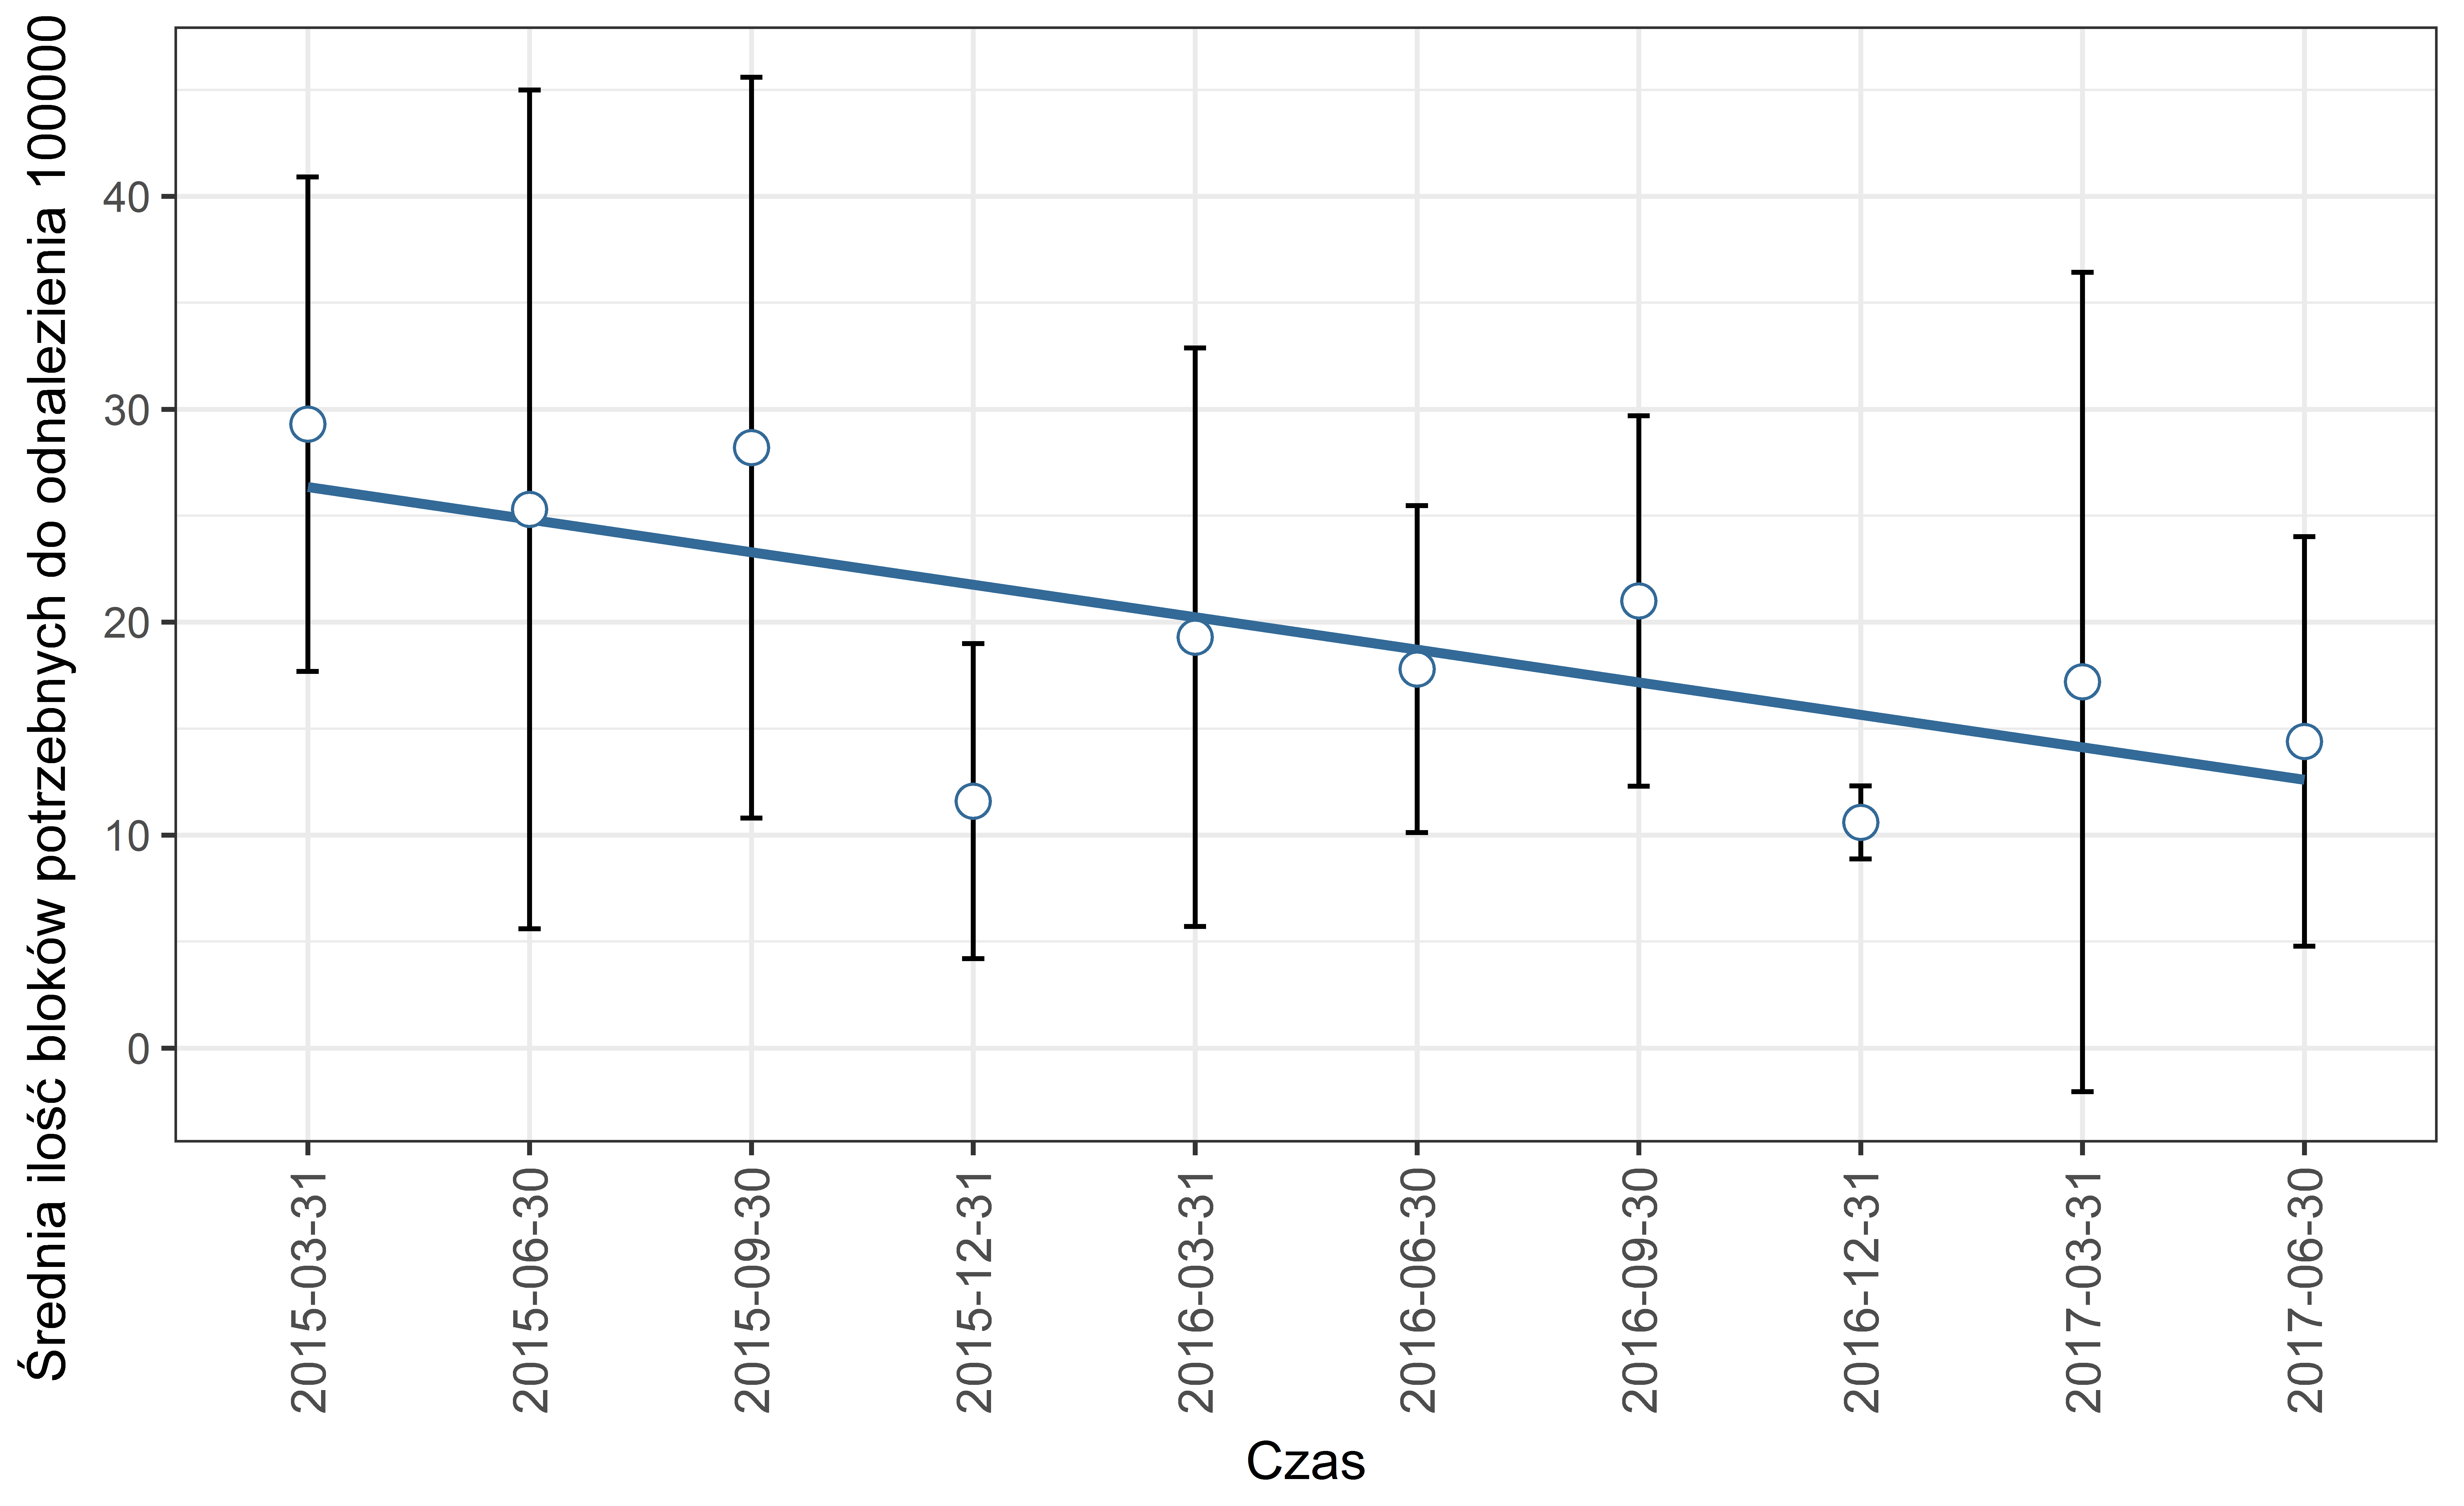
\includegraphics[width=1\linewidth]{pictures/wartosc_transakcji/wartosc_transakcji_sda.png}
%   \caption{}
%   \label{fig:wt2}
%\end{subfigure}
%
%\caption[Średnia wartość transakcji]{(a) mapa cieplna średniej wartości transakcji sieci dla 10 transakcji w 10 okresach (b) regresja liniowa średniej wartości transakcji sieci dla 10 okresów z odchyleniem standardowym}
%
%\end{figure}
%
%\begin{figure}
%\centering
%
%\begin{subfigure}[b]{0.85\textwidth}
%   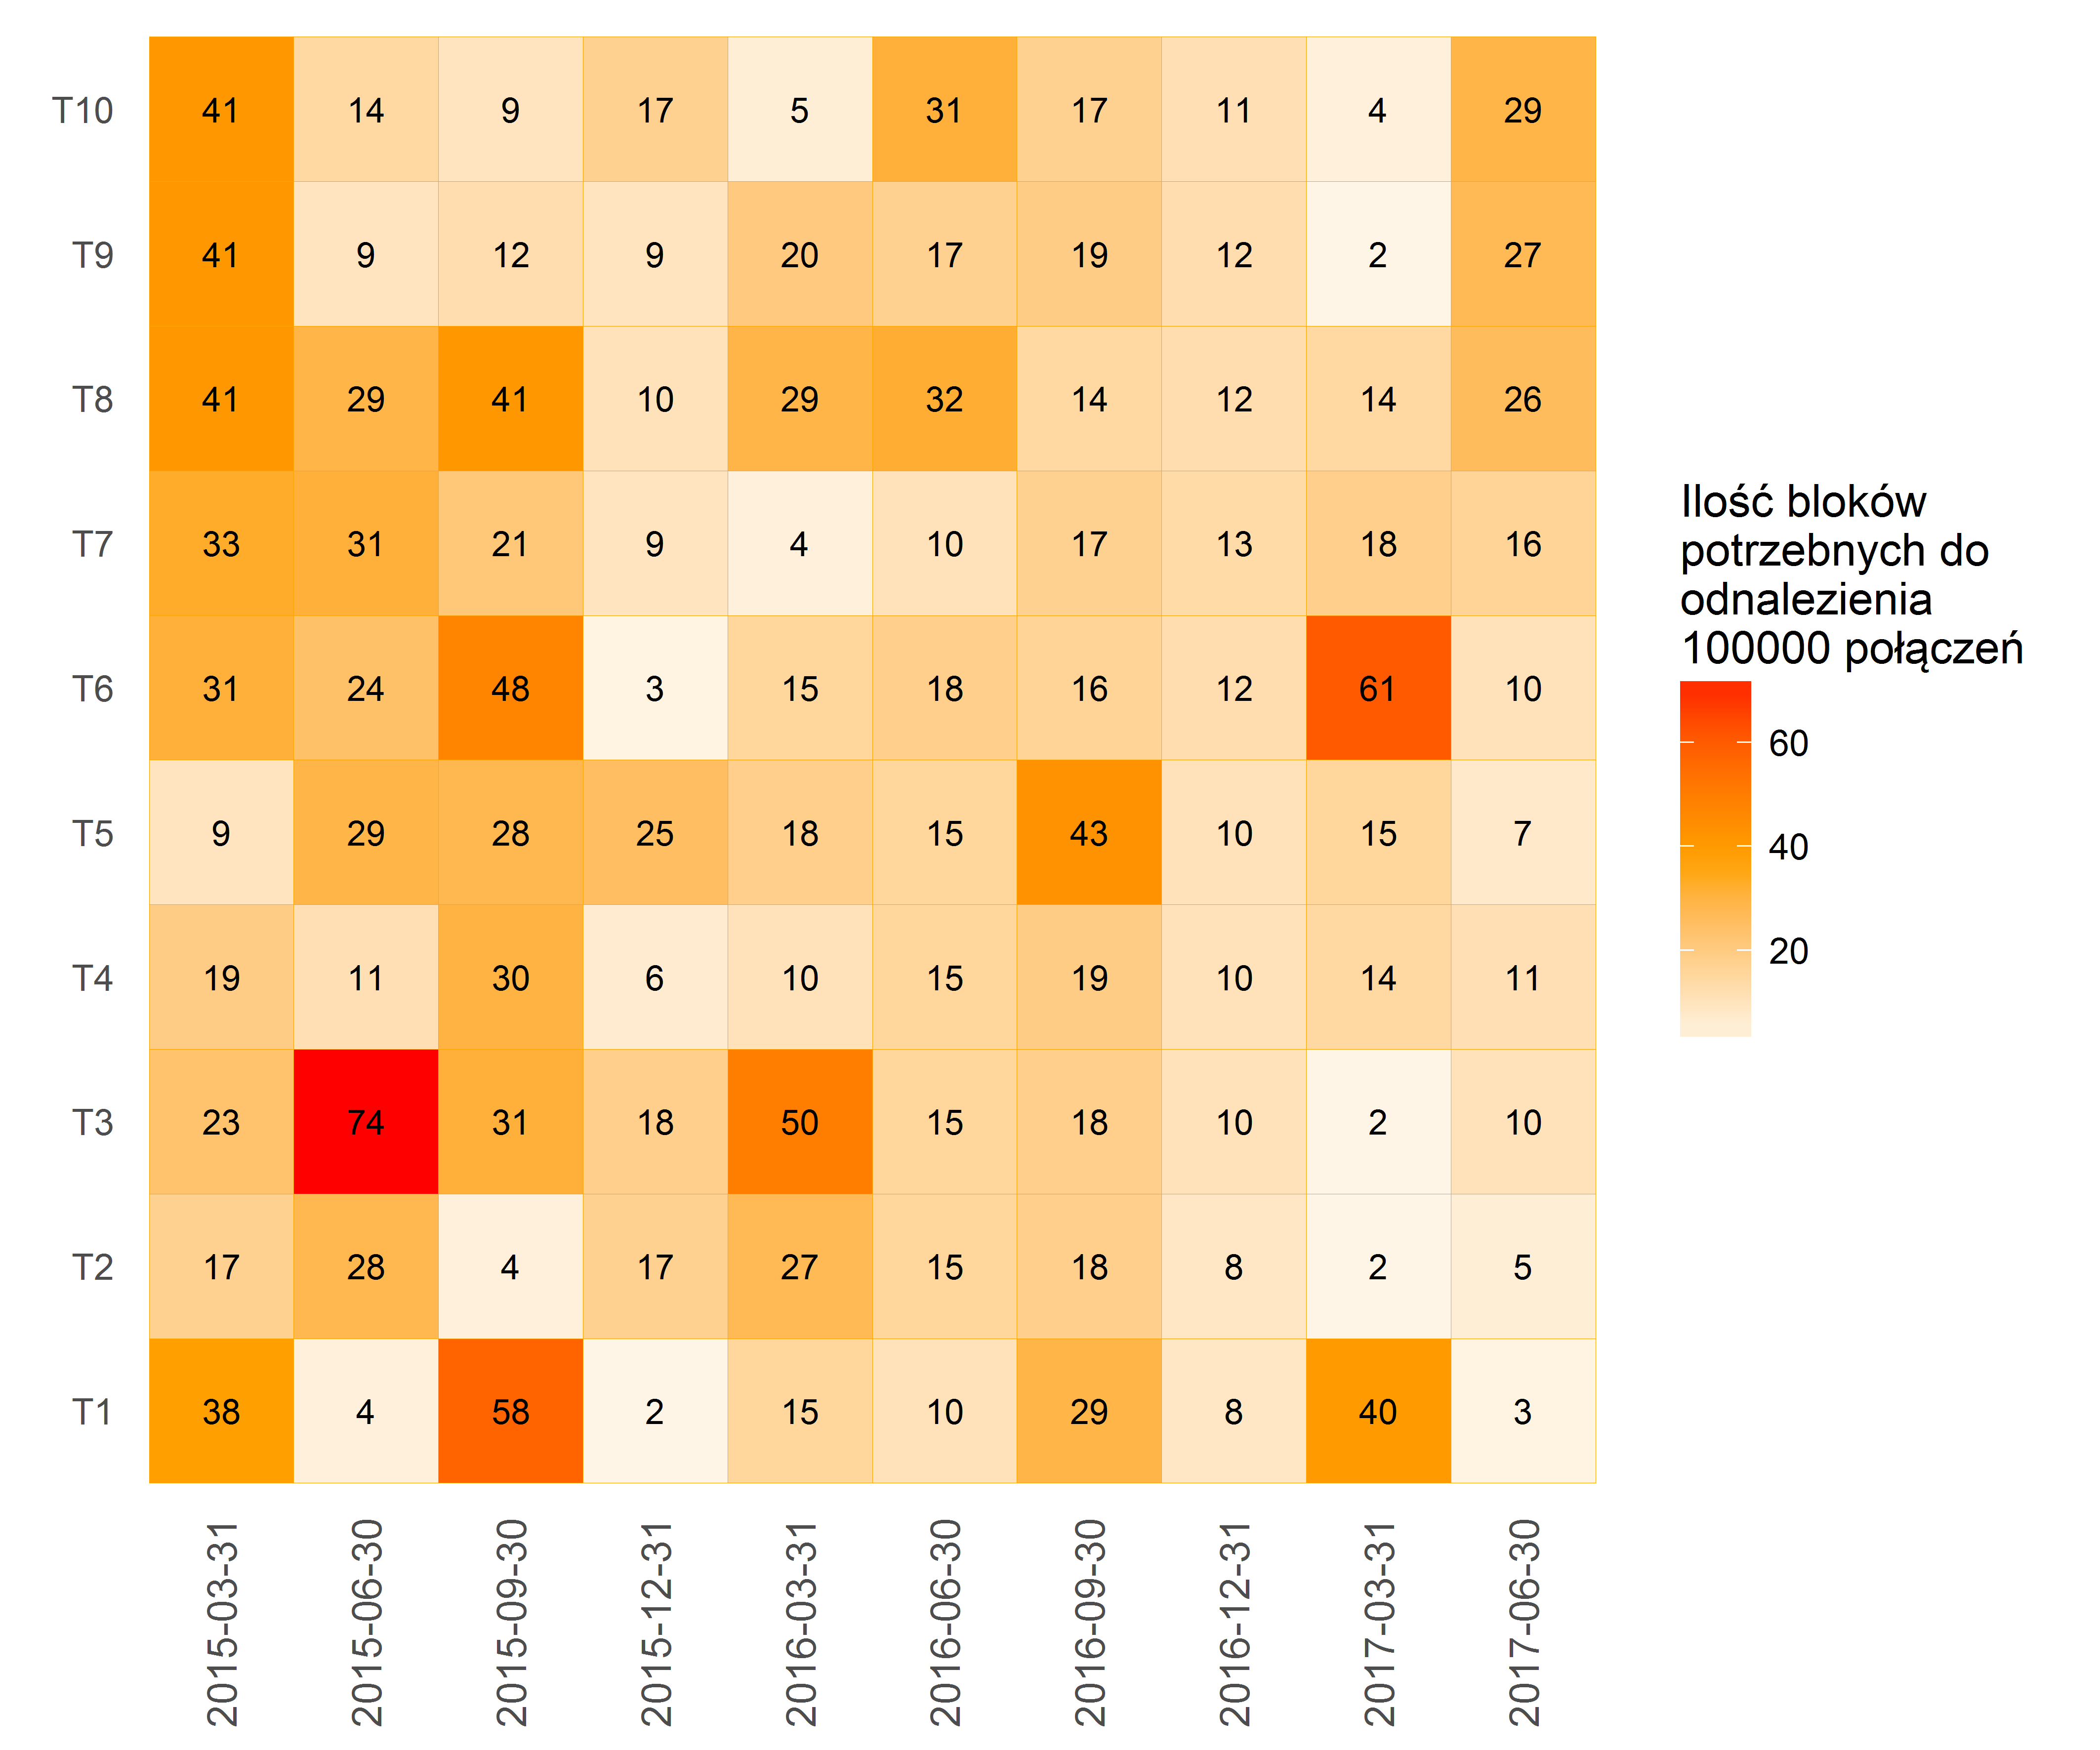
\includegraphics[width=1\linewidth]{pictures/ilosc_blokow/ilosc_blokow_hm.png}
%   \caption{}
%   \label{fig:ib1} 
%\end{subfigure}
%
%\begin{subfigure}[b]{0.85\textwidth}
%   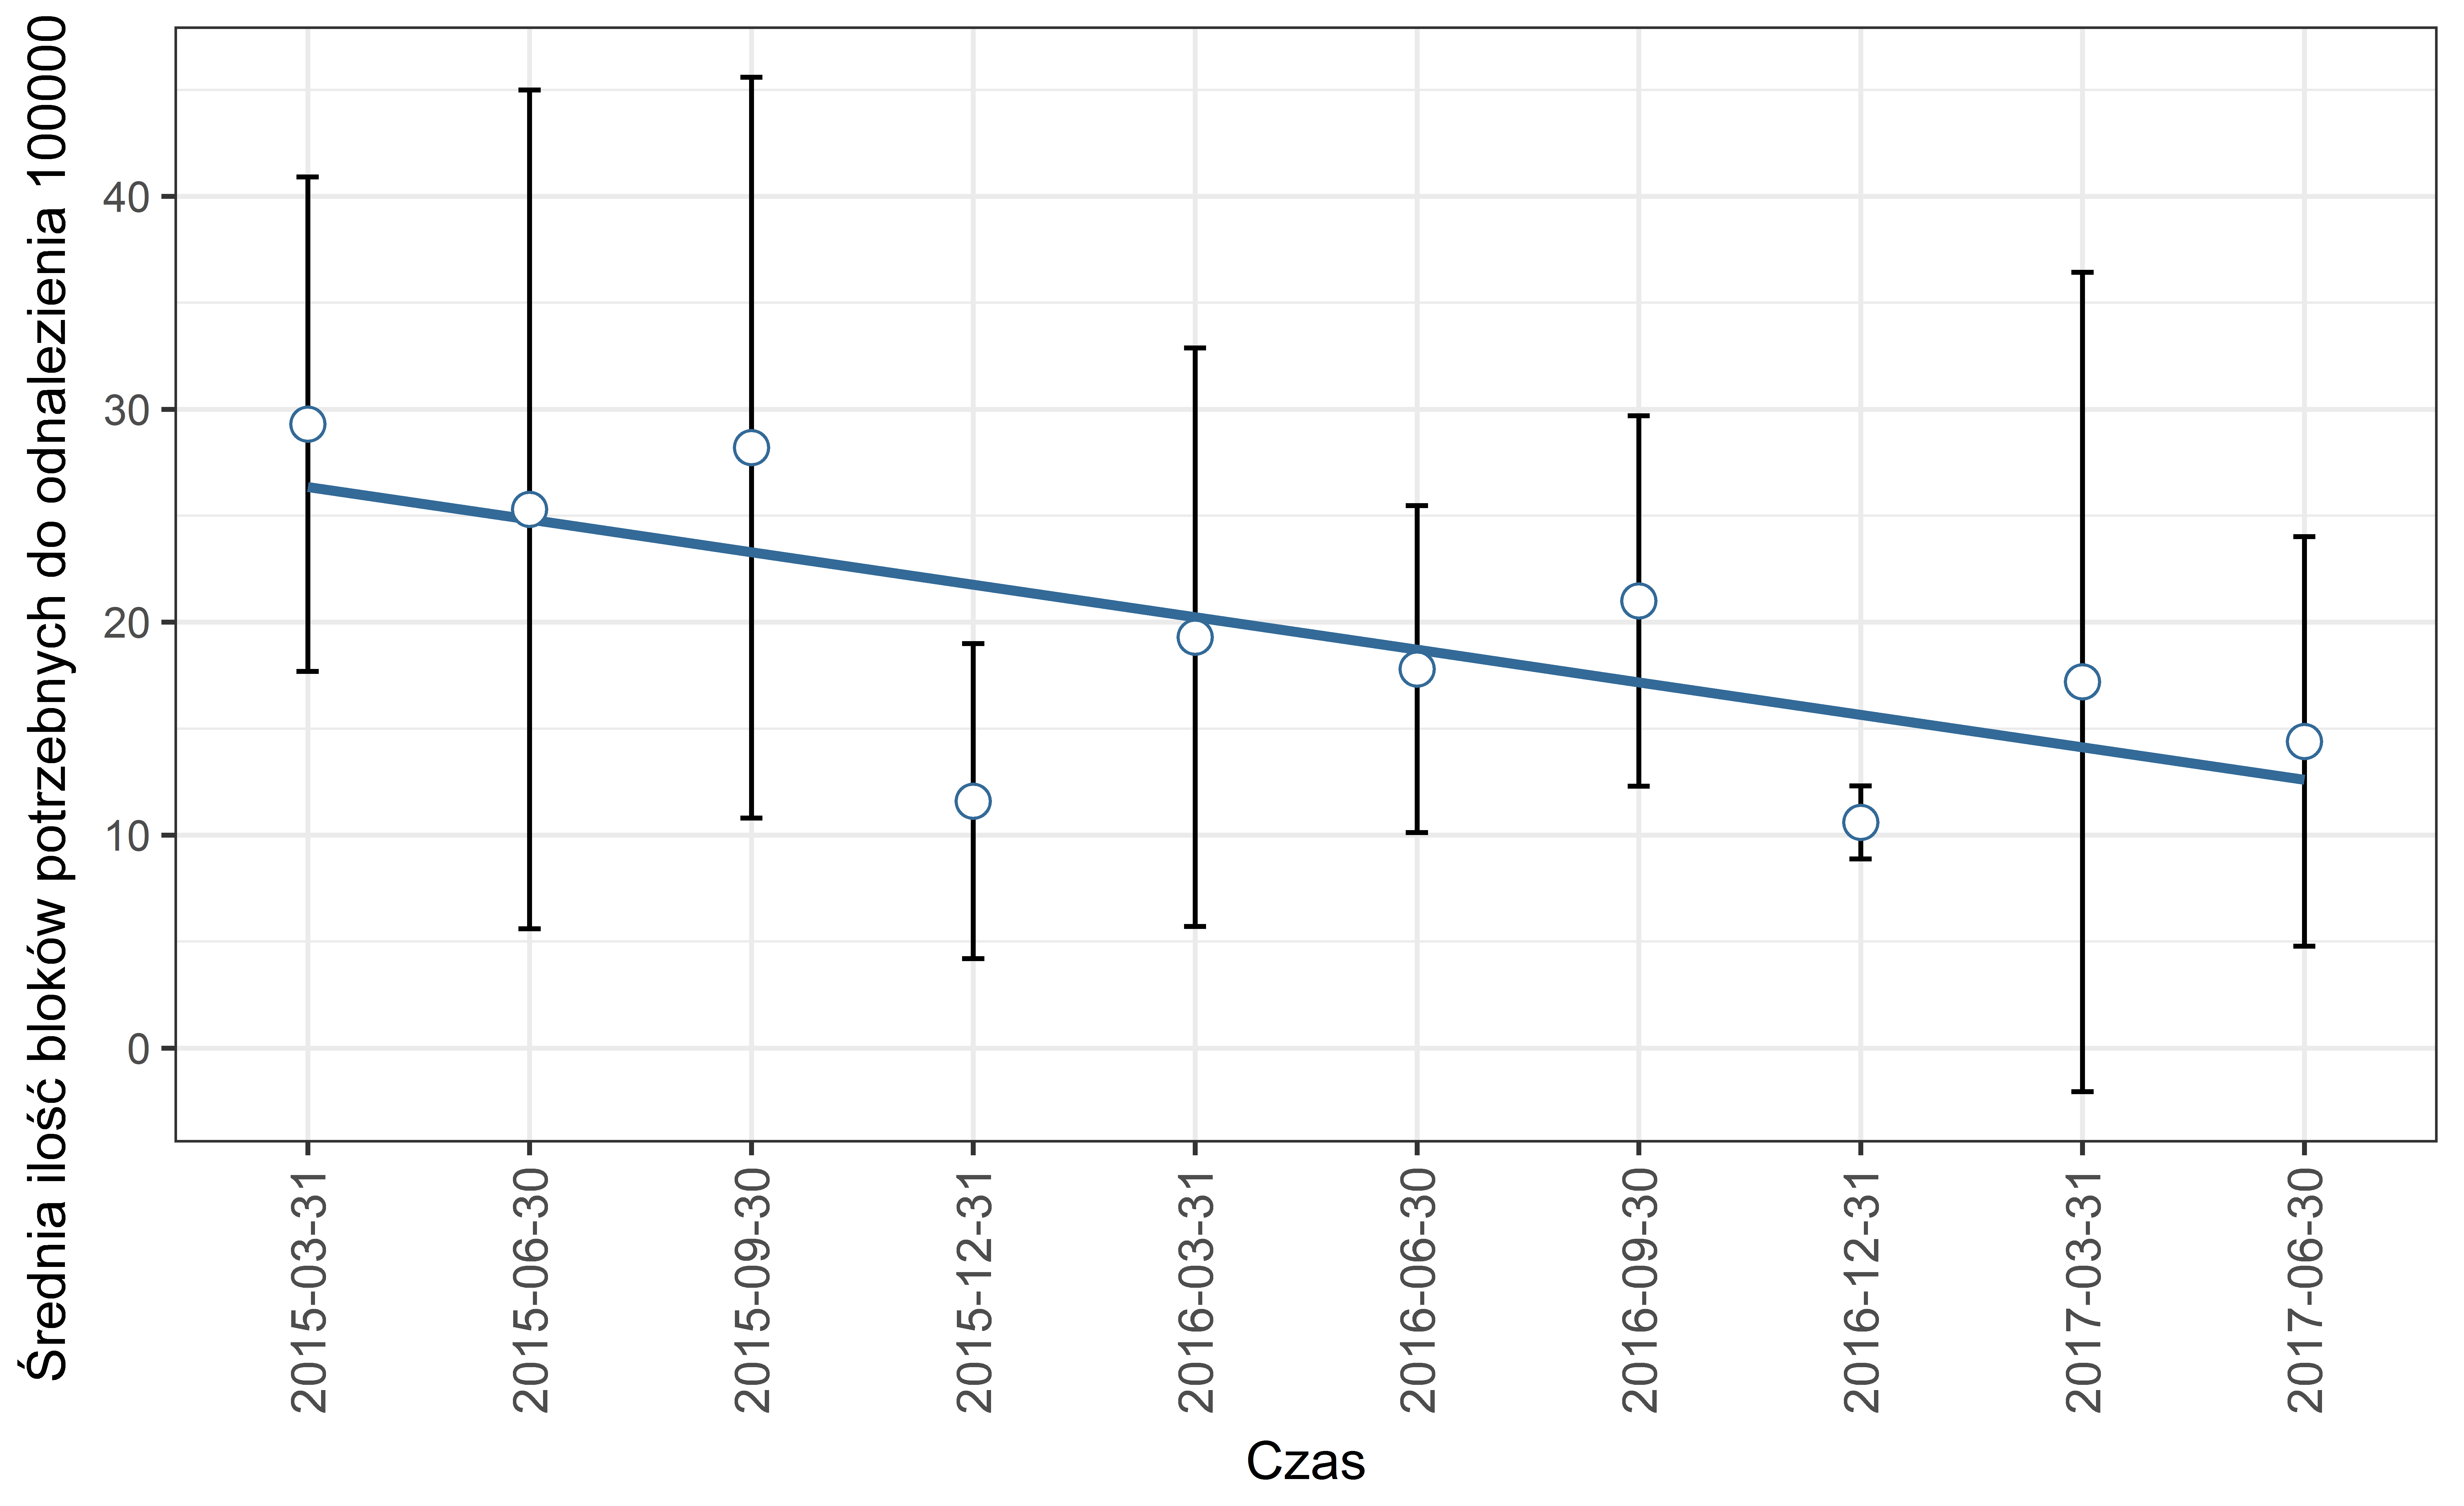
\includegraphics[width=1\linewidth]{pictures/ilosc_blokow/ilosc_blokow_sda.png}
%   \caption{}
%   \label{fig:ib2}
%\end{subfigure}
%
%\caption[Średnia ilość bloków potrzebna na znalezienie 100000 połączeń]{(a) mapa cieplna ilości bloków sieci potrzebnych na znalezienie 100000 połączeń dla 10 transakcji w 10 okresach (b) regresja liniowa ilości bloków sieci potrzebnych na znalezienie 100000 połączeń dla 10 okresów z odchyleniem standardowym}
%
%\end{figure}
%
%\begin{figure}
%\centering
%
%\begin{subfigure}[b]{0.85\textwidth}
%   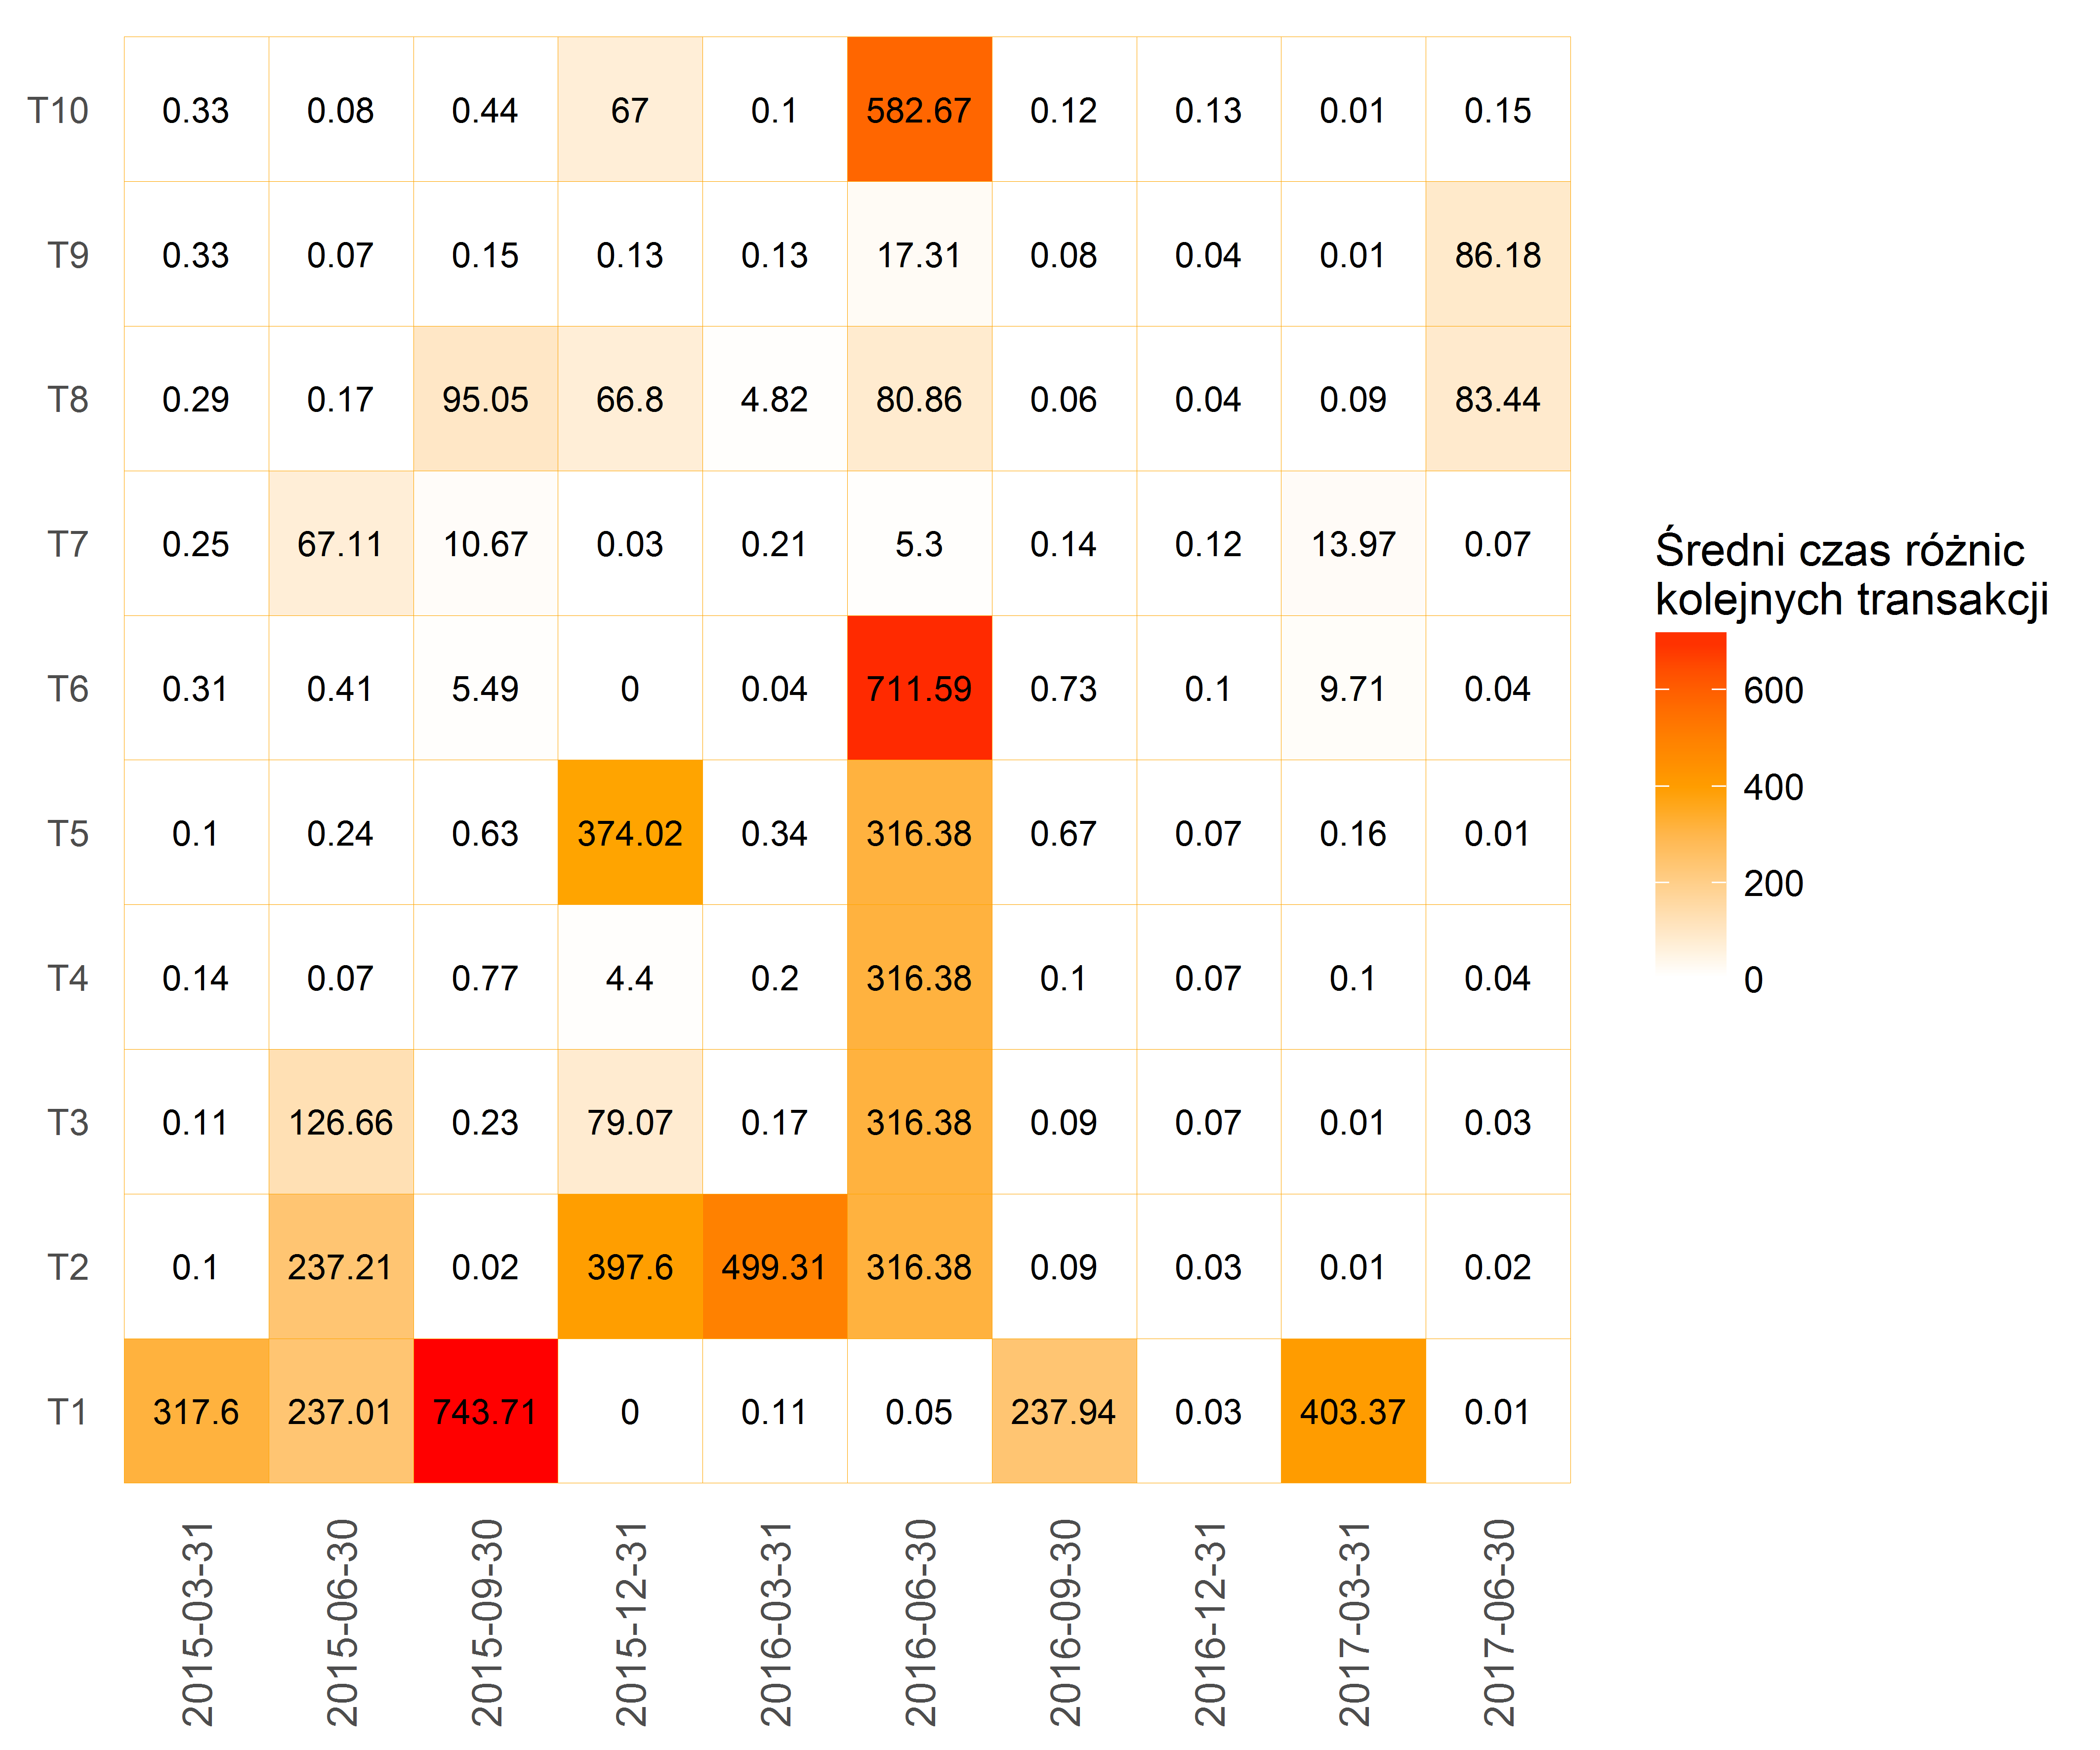
\includegraphics[width=1\linewidth]{pictures/roznica_czasow/roznica_czasow_hm.png}
%   \caption{}
%   \label{fig:rc1} 
%\end{subfigure}
%
%\begin{subfigure}[b]{0.85\textwidth}
%   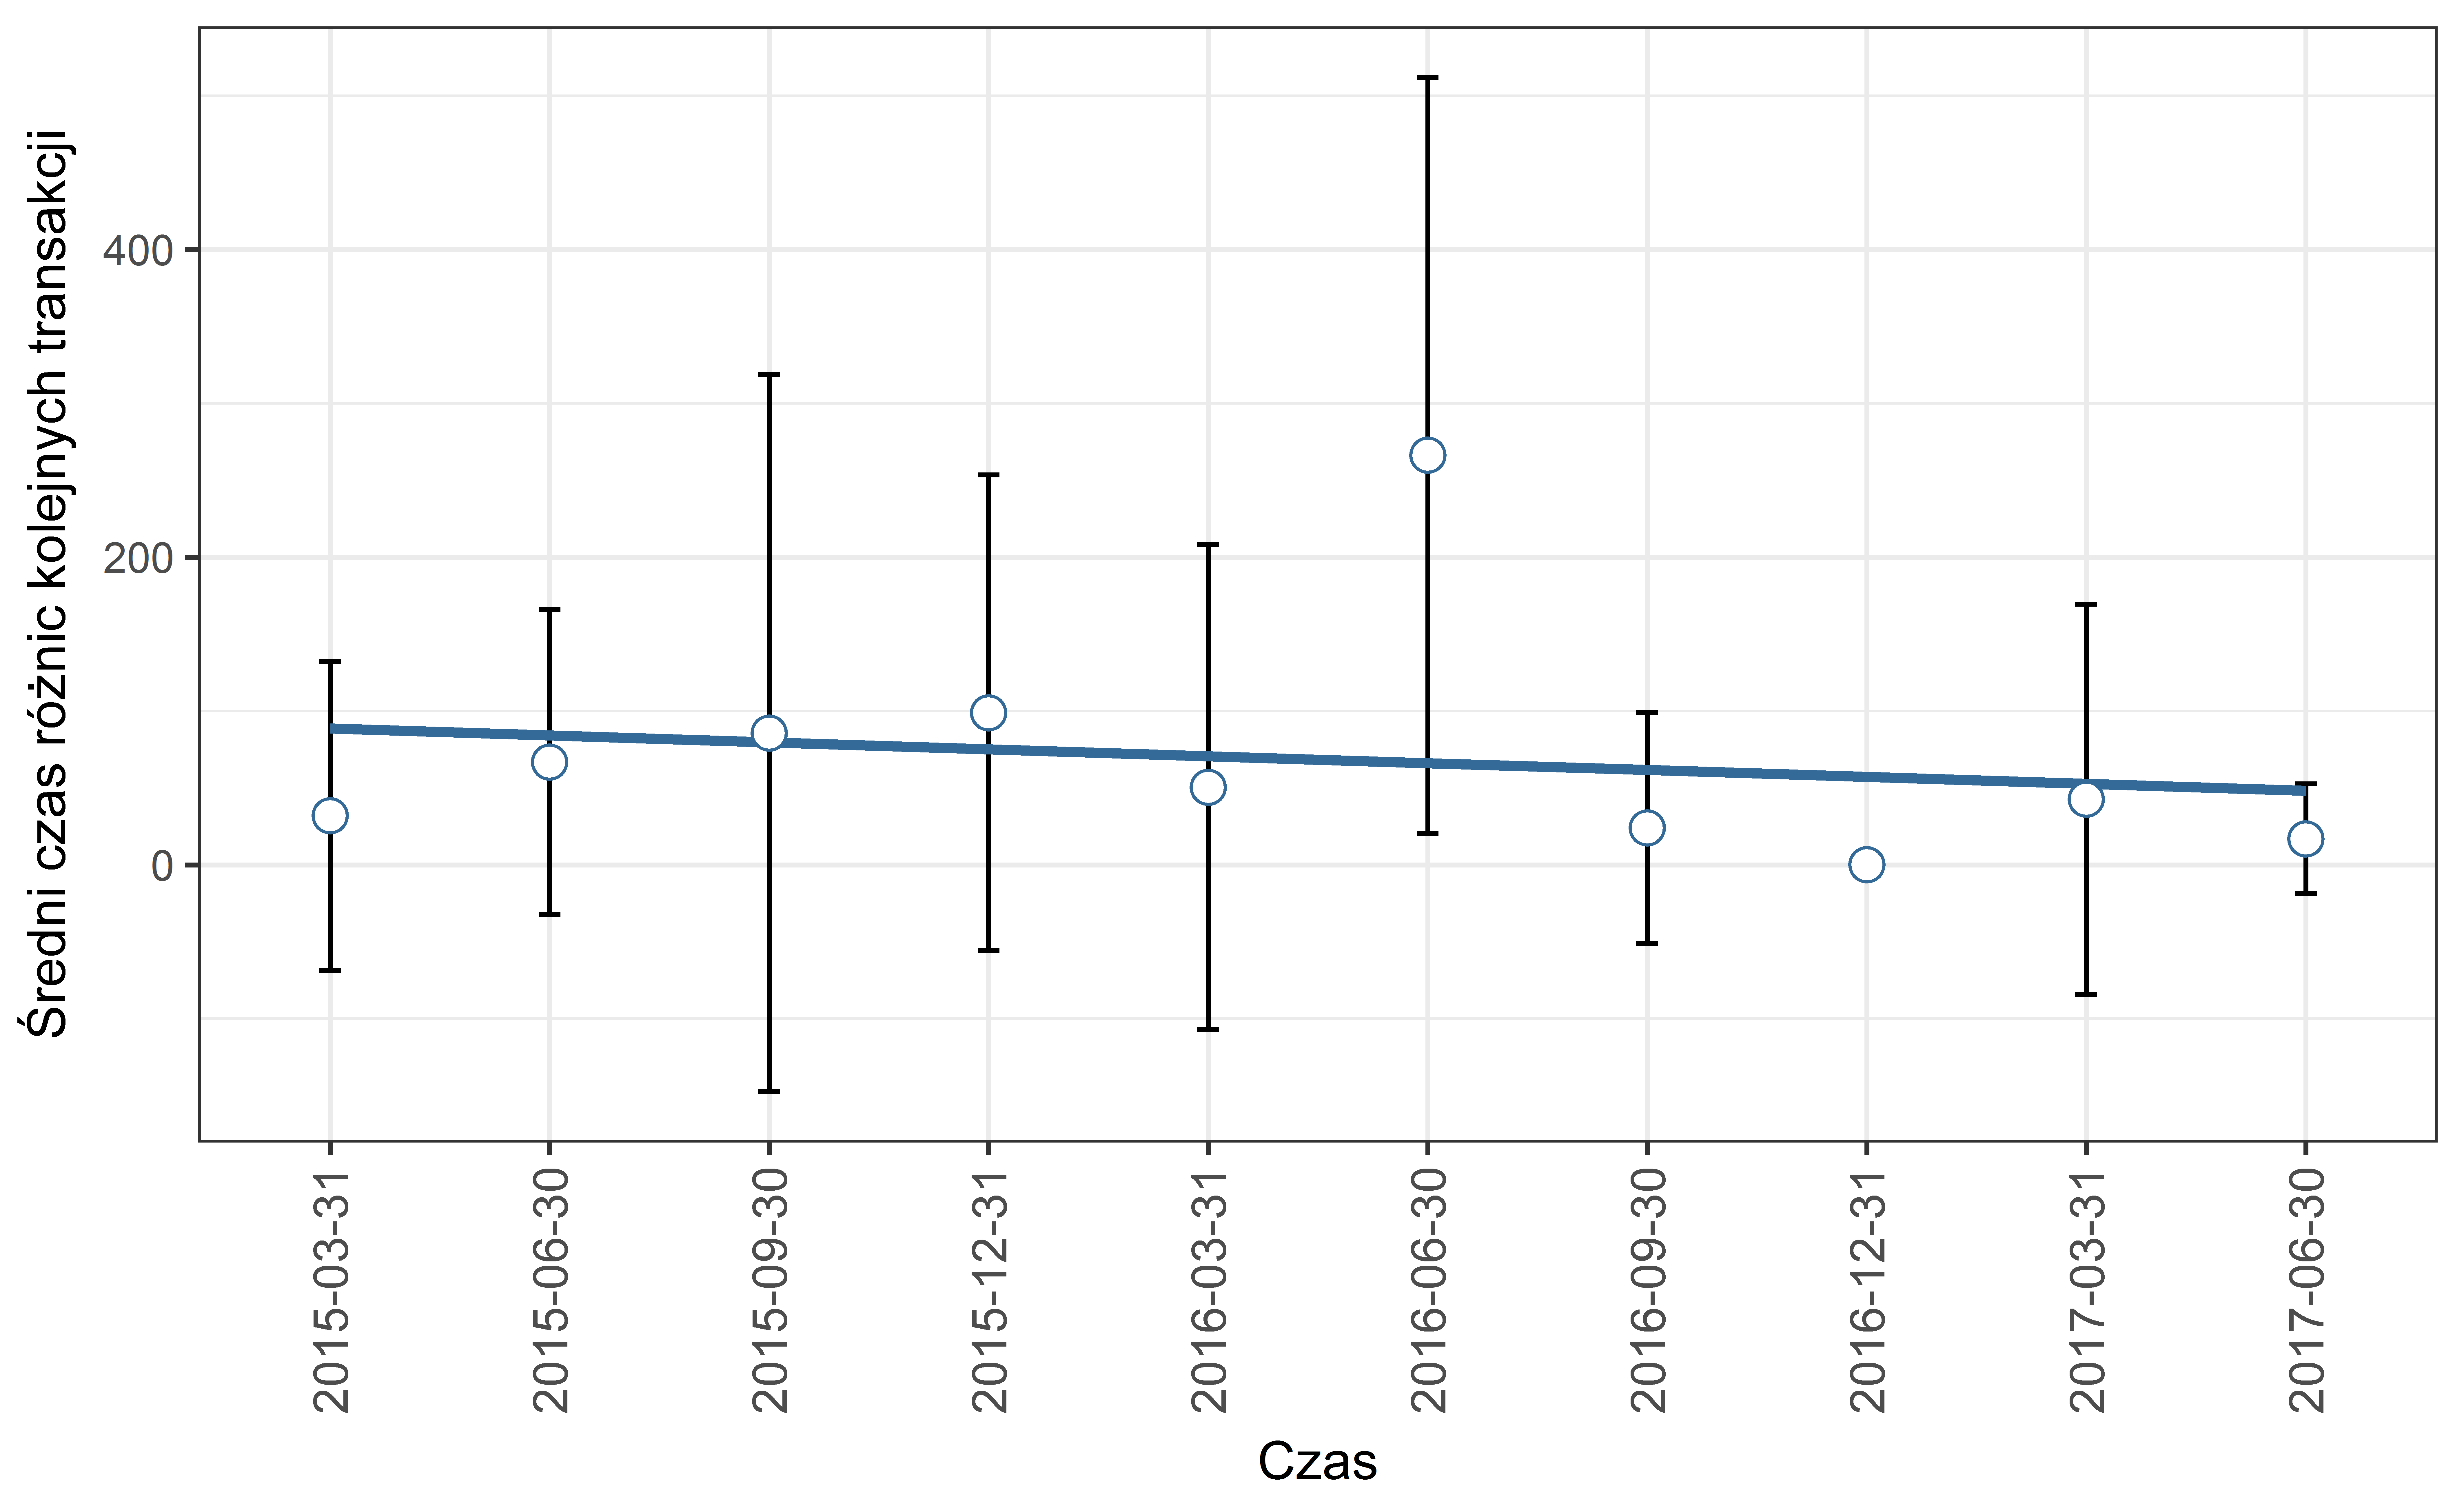
\includegraphics[width=1\linewidth]{pictures/roznica_czasow/roznica_czasow_sda.png}
%   \caption{}
%   \label{fig:rc2}
%\end{subfigure}
%
%\caption[Średni czas różnic kolejnych transakcji]{(a) mapa cieplna średniej różnicy czasu kolejnych transakcji sieci dla 10 transakcji w 10 okresach (b) regresja liniowa średniej różnicy czasu kolejnych transakcji sieci dla 10 okresów z odchyleniem standardowym}
%
%\end{figure}
%
%
%\begin{figure}
%\centering
%
%\begin{subfigure}[b]{0.85\textwidth}
%   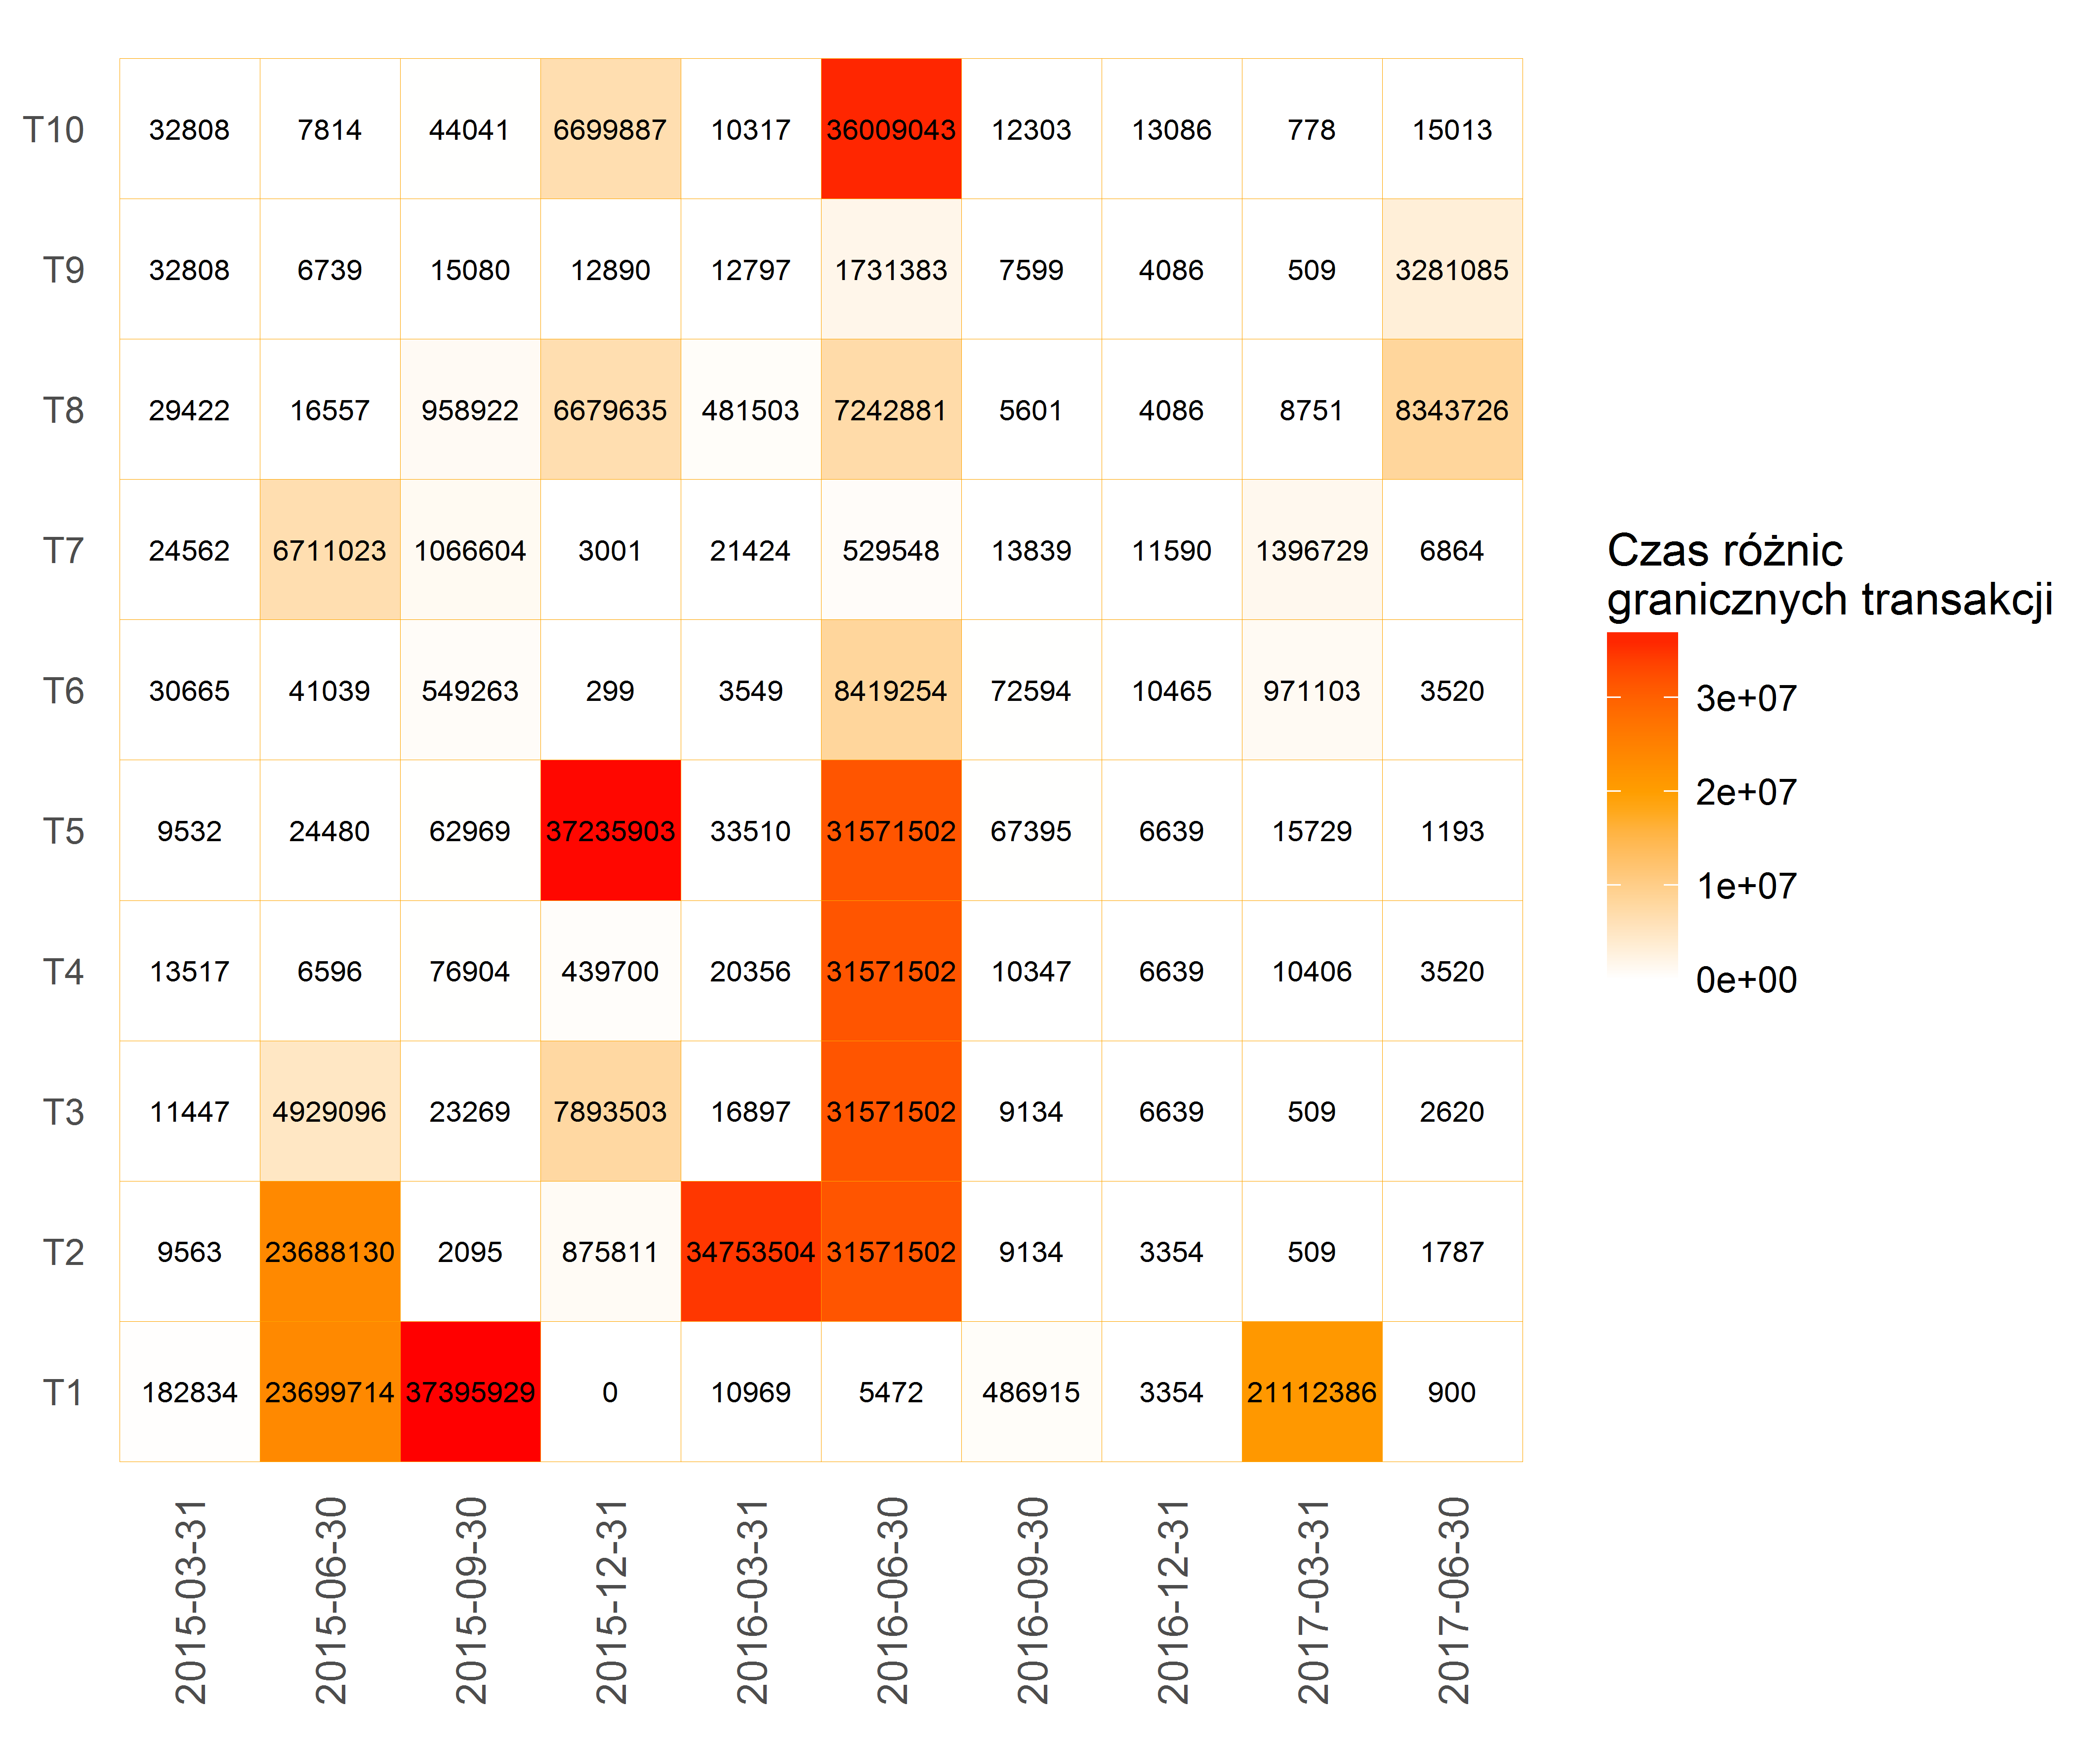
\includegraphics[width=1\linewidth]{pictures/czas_graniczny/czas_graniczny_hm.png}
%   \caption{}
%   \label{fig:cg1} 
%\end{subfigure}
%
%\begin{subfigure}[b]{0.85\textwidth}
%   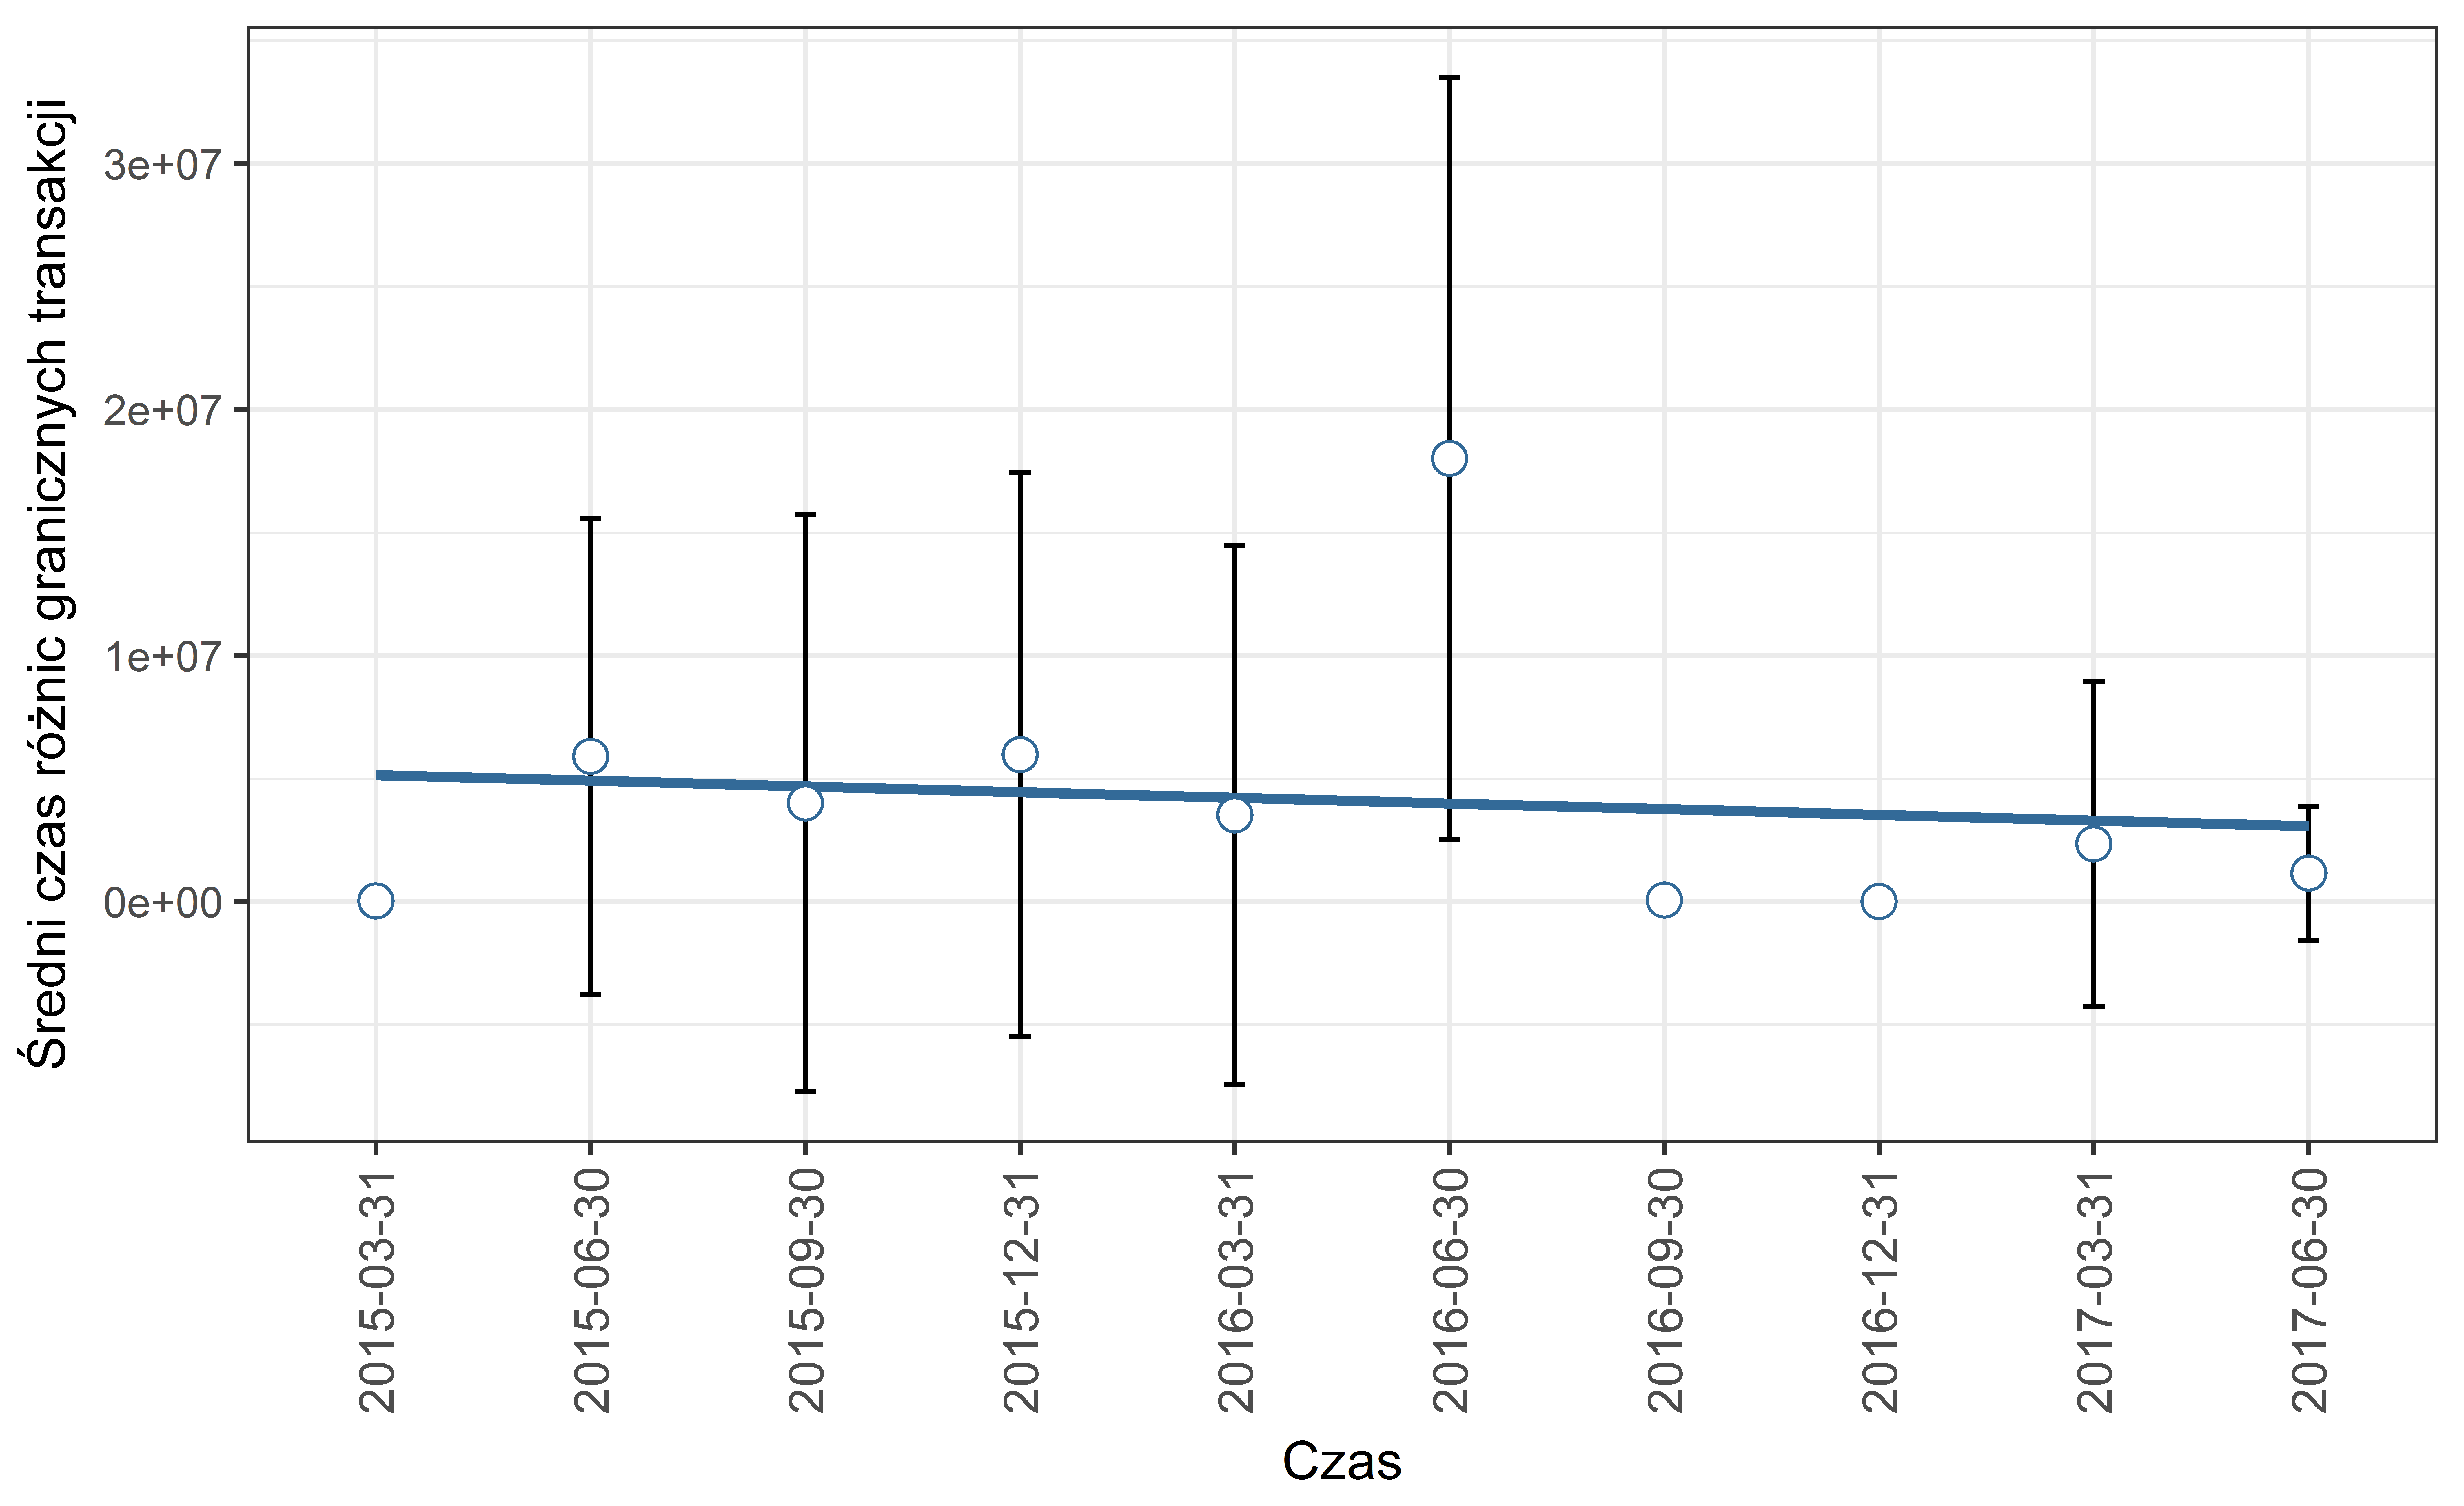
\includegraphics[width=1\linewidth]{pictures/czas_graniczny/czas_graniczny_sda.png}
%   \caption{}
%   \label{fig:cg2}
%\end{subfigure}
%
%\caption[Średni czas różnic granicznych transakcji]{(a) mapa cieplna różnic czasu  granicznych transakcji dla 10 transakcji w 10 okresach (b) regresja liniowa średniego różnic czasu granicznych transakcji dla 10 okresów z odchyleniem standardowym}
%
%\end{figure}

\section{Wnioski}

\chapter{Klasyfikacja w sieci Bitcoin}


\chapter*{Podsumowanie}
\addcontentsline{toc}{chapter}{Podsumowanie}  

\bibliographystyle{unsrt}
\addcontentsline{toc}{chapter}{Bibliografia}
\bibliography{bibliografia2}

\listoffigures
\listoftables
\end{document}

% kropka za numeracja
% 
